%-------------------------------------------------------------------------------
% sequencer64-user-manual
%-------------------------------------------------------------------------------
%
% \file        sequencer64-user-manual.tex
% \library     Documents
% \author      Chris Ahlstrom
% \date        2015-11-01
% \update      2016-10-01
% \version     $Revision$
% \license     $XPC_GPL_LICENSE$
%
%     This document provides LaTeX documentation for Sequencer64.
%
%-------------------------------------------------------------------------------

\documentclass[
 11pt,
 twoside,
 a4paper,
 headinclude,
 footinclude,
 final                                 % versus draft
]{article}

%-------------------------------------------------------------------------------
% docs-structure
%-------------------------------------------------------------------------------
%
% \file        docs-structure.tex
% \library     Documents
% \author      Chris Ahlstrom
% \date        2015-04-20
% \update      2016-02-28
% \version     $Revision$
% \license     $XPC_GPL_LICENSE$
%
%     This "include file" provides LaTeX options for a document.
%
%     Note that enumitem is an extension of enumerate, and comes from
%     Debian's texlive-latex-recommended package.
%
%-------------------------------------------------------------------------------

\usepackage{enumitem}         % setting the whitespace between and within lists
\setlistdepth{9}
% \setlist{nosep}             % spacing around the list
\setlist{noitemsep}           % spacing within the list

% \usepackage[dvipsnames]{xcolor} % provide more colors?

\usepackage{color}            % provide colors?

% \usepackage[usenames,dvipsnames,svgnames,table]{xcolor}

\usepackage{nameref}          % Provide references by name instead of number
\usepackage[colorlinks=true,linkcolor=webgreen,filecolor=webbrown,citecolor=webgreen]{hyperref}
\definecolor{webgreen}{rgb}{0,.5,0}
\definecolor{webbrown}{rgb}{.6,0,0}

\usepackage{url}              % Required for including URLs
\usepackage{hyperref}         % Required for including hyperlinks
\usepackage{amsthm}           % Helps avoid "destination with same
% \usepackage{cleveref}       % identifier" warnings?
\usepackage[hypcap]{caption}  % make labels point to figure, not the caption
% \usepackage{hypcap}         % make labels point to figure, not the caption
\usepackage[pdftex]{graphicx} % Required for including images
\graphicspath{{../images/}}   % Set the default folder for images
\usepackage{float}            % For more control of location of Figures
\usepackage{geometry}         % Page & text layout
\geometry{
  letterpaper,
  top=2.5cm,
  bottom=2.5cm,
  left=2cm,
  right=2cm
}

\usepackage{longtable}        % For making multi-page tables
\usepackage{makeidx}          % For making an index

% Let's try to reduce the size of quotations.

\usepackage{relsize,etoolbox}          % http://ctan.org/pkg/{relsize,etoolbox}
\AtBeginEnvironment{quotation}{\smaller}   % Step font down one size relatively

% Doesn't seem to do anything:
%
% \usepackage{titlesec}         % for reducing space before headings
% \titlespacing*{\section}{0pt}{1.0\baselineskip}{\baselineskip}
% \titlespacing*{\subsection}{0pt}{1.0\baselineskip}{\baselineskip}
% \titlespacing*{\subsubsection}{0pt}{1.0\baselineskip}{\baselineskip}

% This package isn't available easily on CentOS:
%
% \usepackage[subtle]{savetrees} % For tightening document vertical spacing

\hypersetup{                  % HYPERLINKS
% draft,                      % Uncomment removes links (e.g. for B&W printing)
 colorlinks=true,
 breaklinks=true,
% bookmarks=true,
 bookmarksnumbered,
 urlcolor=webbrown,
 linkcolor=blue,              % RoyalBlue
 citecolor=webgreen,
 pdftitle={},
 pdfauthor={\textcopyright},
 pdfsubject={},
 pdfkeywords={},
 pdfcreator={pdfLaTeX},
 pdfproducer={LaTeX with hyperref and ClassicThesis}
}

% Make an "enumber" style that makes all levels of enumerated lists show
% arabic numerals.

\newlist{enumber}{enumerate}{10}
\setlist[enumber]{nolistsep,label=\arabic*.}

% Make "paragraph" a fourth level, and make it shown in the table of
% contents.

\makeatletter
\renewcommand\paragraph{\@startsection{paragraph}{4}{\z@}%
   {-2.5ex\@plus -1ex \@minus -.25ex}%
   {1.25ex \@plus .25ex}%
   {\normalfont\normalsize\bfseries}}
\makeatother
\setcounter{secnumdepth}{4} % how many sectioning levels to assign numbers to
\setcounter{tocdepth}{4}    % how many sectioning levels to show in ToC

% Provide a way of counting user interface items without putting them in an
% enumberation.

\newcounter{ItemCounter}

% Makes a numbered paragraph out of an item, and allows two index entries
% for it.

\newcommand{\itempar}[2] {
   \stepcounter{ItemCounter}
   \textbf{\arabic{ItemCounter}. #1.}
   \index{#1}
   \index{#2}
}

% Provides for two forms of an option, as might be shown in a man page.

\newcommand{\optionpar}[2] {
   \textbf{\texttt{#1}} \textbf{\texttt{#2}} \\
   \index{#1}
   \index{#2}
}

% Now deprecated in preference to \itempar

\newcommand{\settingdesc}[2] {
   \textbf{#1}
   \index{#1}
   \index{#2}
}

% Make a full reference to a figure using its number, its name, and its page
% number.  Very useful if you have a hard-copy of the document to deal with.

\newcommand{\figureref}[1] {
   figure~\ref{#1}
   ("\nameref{#1}")
   on page~\pageref{#1}\ignorespaces
}

% Make a full reference to a section using its number, its name, and its page
% number.  Very useful if you have a hard-copy of the document to deal with.

\newcommand{\sectionref}[1] {%
   section~\ref{#1}
   ("\nameref{#1}")
   on page~\pageref{#1}\ignorespaces
}

% Make a full reference to a "paragraph"  using its number, its name, and
% its page number.  Very useful if you have a hard-copy of the document to
% deal with.

\newcommand{\paragraphref}[1] {%
   paragraph~\ref{#1}
   ("\nameref{#1}")
   on page~\pageref{#1}\ignorespaces
}

% Make a full reference to a table using its number, its name, and its page
% number.  Very useful if you have a hard-copy of the document to deal with.

\newcommand{\tableref}[1] {%
   table~\ref{#1}
   ("\nameref{#1}")
   on page~\pageref{#1}\ignorespaces
}

% For lining up enumerated items.  Doesn't really work well, better
% to create a table.

\newcommand{\itab}[1]{\hspace{0em}\rlap{#1}}
\newcommand{\tab}[1]{\hspace{.1\textwidth}\rlap{#1}}

% An attempt to reduce excess vertical space.  Does not work.  See the
% top of yoshimi-user-manual.tex instead.
%
% \setlength{\parindent}{0pt}
% \setlength{\parskip}{0pt}

% Space between floats. \dblfloatsep for 2 column format.
% \setlength{\floatsep}{8pt}

% Space above and below in-line text floats
% \setlength{\intextsep}{8pt}

% Space above float caption
% \setlength{\abovecaptionskip}{8pt}

% Space below float caption
% \setlength{\belowcaptionskip}{8pt}

% Change the fragction of the page that can be filled with graphics from 0.7
% to 0.9.

\renewcommand\floatpagefraction{.9}
\renewcommand\dblfloatpagefraction{.9}
\renewcommand\topfraction{.9}
\renewcommand\dbltopfraction{.9}
\renewcommand\bottomfraction{.9}

\raggedbottom                          % avoid excessive vertical justification

%-------------------------------------------------------------------------------
% vim: ts=3 sw=3 et ft=tex
%-------------------------------------------------------------------------------
                 % specifies document structure and layout

% Replacing normal header/footer with a fancier version.  These two symbols of
% document class were showing up as "unused" in the log file.
%
% headinclude,
% footinclude,
%
% So we add the fancyhdr package, clear the default layout, and set it up for
% our wider pages.

\usepackage{fancyhdr}
\pagestyle{fancy}
\fancyhead{}
\fancyfoot{}
\fancyheadoffset{0.005\textwidth}
\lhead{Sequencer64 Live MIDI Sequencer}
\chead{}
\rhead{User Manual}
\lfoot{}
\cfoot{\thepage}
\rfoot{}

\makeindex

\begin{document}

\title{Sequencer64 User Manual 0.9.18}
\author{Chris Ahlstrom \\
   (\texttt{ahlstromcj@gmail.com})}
\date{\today}
\maketitle

\begin{figure}[H]
   \centering 
   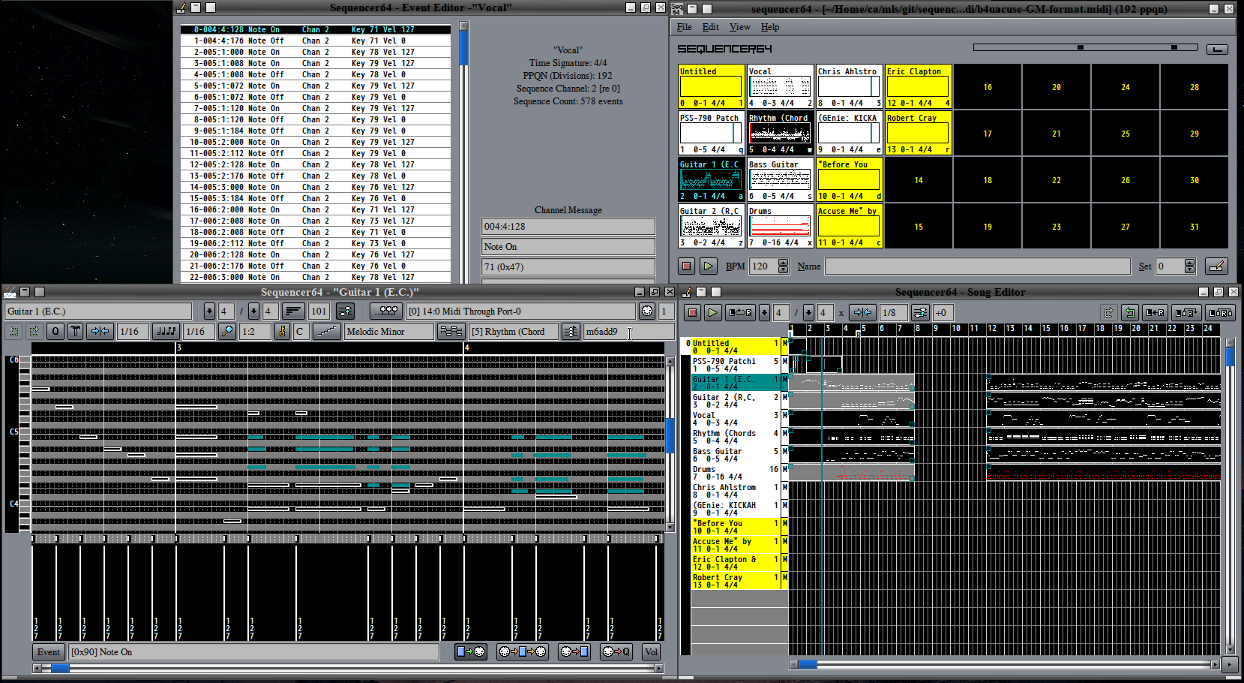
\includegraphics[scale=0.50]{Sequencer64-0_9_17.png}
\end{figure}

\clearpage                             % moves Contents to next page

\tableofcontents
\listoffigures                         % print the list of figures
\listoftables                          % print the list of tables

% Changes the paragraph style to remove indenting and put a line between each
% paragraph.  This could be moved up into the preamble, but then would
% affect the spacing of the TOC and LOF, LOT noted above.

\setlength{\parindent}{0pt}
\setlength{\parskip}{1ex plus 0.5ex minus 0.2ex}

\section{Introduction}
\label{sec:introduction}

   This document describes how to use \textsl{Sequencer64}
   \cite{sequencer64}, through version 0.9.18,
   using the latest commit from the
   \textbf{master} or \textbf{fixups} branches.
   If one is impatient to get started mastering \textsl{Sequencer64},
   then proceed to \sectionref{subsec:introduction_lets_get_started}.

   \textsl{Sequencer64} fixes some bugs in JACK support, MIDI clocking, and
   JACK Master mode (with code from the \textsl{SooperLooper} 
   and \textsl{Seq32} projects).
   However, as user \textsl{stazed} notes on GitHub, there is more that can be
   done (and he has done much with his \textsl{seq32} \cite{seq32} project).

   We've added a many features to make song editing more
   convenient.
   There is now a Pause button and keystroke, (defaults to a period, ".").
   Much more editing and navigation can be done using keystrokes.
   A shift-left-click on a pattern slot in the pattern window,
   or on a pattern's name or M button in the song editor toggles the armed or
   mute status of all of the \textsl{other} active patterns.
   We've got zoom keys for the editors, current-sequence highlighting,
   a raft of important bug fixes, some optimization, and much more.

   We have many contributors to acknowledge.  Please see
   \sectionref{sec:kudos}.

\subsection{Sequencer64: What?}
\label{subsec:what_is_sequencer64}

   \textsl{Sequencer64} is an continuation of of \textsl{Seq24},
   a live-looping sequencer with an interface more like a hardware sequencer
   than the typical software MIDI sequencer.
   \textsl{Sequencer64} has many updates and improvements, and a modestly
   new look, so that a new manual is a necessity.

   \textsl{Seq24} was, a few years back, a very active project, with a
   number of contributors, who have created patches, additional
   functionality, and even ports to Windows.
   We searched assiduously for these updates, and
   incorporated most of them into \textsl{Sequencer64} where feasible.
   There are still some things to be done, including a port to
   Windows/Portmidi.

   \textsl{Sequencer64} is not a synthesizer.  It requires a hardware
   synthesizer, or a software synthesizer such as Timidity \cite{timidity},
   FluidSynth \cite{fluidsynth}, ZynAddSubFX \cite{zynaddsubfx}, Yoshimi
   \cite{yoshimi} \cite{yoshimi2}, AmSynth \cite{amsynth}, Bristol
   \cite{bristol}, and others (see \cite{linuxsynths} for a fairly
   comprehensive list of "Linux" synthesizers).

   \textsl{Sequencer64}, like \textsl{Seq24},
   works a bit like an \textsl{Alesis SR16} drum machine,
   which, for some, is a very intuitive and fast way to do MIDI.
   If one has worked with trackers like \textsl{SoundTracker} and
   \textsl{ShakeTracker}, then "you are a tracker guy and it gonna go fast".
   With \textsl{Sequencer64}, one creates several patterns, and then
   combines them.

   Now, unfortunately, \textsl{Seq24} spent some time in limbo
   (2010 was the last major update, with a
   recent update to fix a MIDI clock issue).  There are a number of
   forks for it on \textsl{GitHub}, and some conversions
   to code in other languages, and some patches.
   There is also a fairly extensive port to Windows.
   So, why would we bother creating yet another fork of \textsl{Seq24}?

\subsection{Sequencer64: Why?}
\label{subsec:introduction_seq64_vs_others}

   The first reason to reboot \textsl{Seq24} is consolidation of many of the
   features and fixes that it has accumulated in various forks over the years.
   Also, although "feature-complete", additional features would be useful, such
   as support for more session managers, more use of keystrokes, work-arounds
   for the need for two mouse buttons, a more up-to-date user-interface
   framework, more comprehensive undo/redo, bug fixes, beefing up the
   support for the "user" configuration file, and a way to edit parts of the
   MIDI file textually.

   We view \textsl{Seq24} as a kind of "vi" of MIDI editing... spare, lean, and
   powerful.  Without \textsl{Seq24} and its authors, \textsl{Sequencer64}
   would never have come into being.

\subsection{Improvements}
\label{subsec:improvements}

   The following improvements have been made to \textsl{Seq24} for
   \textsl{Sequencer64}.

   \begin{itemize}
      \item A new \textsl{event editor} dialog was added.
         It detailed viewing and editing of MIDI events.
         This editor is basic, but useful.
      \item \textsl{Sequencer64} reads SMF 0 MIDI files.  It splits
         the file into tracks based on channel number.  Each track becomes one
         sequence/pattern in the main window grid.
      \item A "Tap" button for setting the BPM by tapping a button or a key.
      \item Some features have been ported from \textsl{Stazed}'s
      \textsl{Seq32} \cite{seq32} project.  Some features can be disabled at
      configure/build time, if desired.
      \begin{itemize}
         \item The chord-generation feature of \textsl{Seq32}.
         \item The pattern-transposing feature.
         \item MIDI song export.
            It allows a song/performance to be exported into a MIDI file
            without \textsl{Sequencer64} loops, so that the performance can be
            played in a standard MIDI sequencer.
         \item The extended undo/redo support of \textsl{Seq32} has been
            ported to \textsl{Sequencer64}.
         \item The ability to split triggers at the nearest snap, instead
            simply splitting them in half.
         \item A large number of other \textsl{Seq32} features have been
            ported, but they are currently commented out until we can test them
            and make sure they are "perfect".
         \begin{itemize}
            \item Enhanced JACK support.
            \item Diverting multi-channel recorded MIDI so that each channel
               is stored in the sequence/pattern configured for that channel
            \item Randomizing MIDI events.
            \item Selection extensions such as selecting odd/even notes, and
            handles on data events.
            \item More feature for controlling transport.
            \item Support for editing the amplitude of data events using a
               low-frequency oscillator (LFO).
         \end{itemize}
      \end{itemize}
      \item One can optionally bring up two song editor windows, to have a view
         of two different parts of a large song while arranging it.
      \item The Set Tempo and Time Signature events of normal MIDI files are
         now processed and incorporated into the user-interface and are saved
         as standard MIDI data.
      \item One can now save the scale, key, and background sequence
         settings to the \textsl{Sequencer64} MIDI file, either globally or
         per-sequence.
      \item In the sequence/pattern and song editors, the window now scrolls to
         keep up with the progress bar for sequences that are longer than the
         width of the sequence editor window.
      \item Additional mouse and keystroke support in the pattern and song
         editor windows:
      \begin{itemize}
         \item Usage of Page Up, Page Down, and Shift Page Up, Shift Page Down,
            to move vertically and horizontally in the pattern and song
            windows.
         \item Moving selected notes or triggers using the arrow keys.
         \item Pasting selected notes (and other events) using the arrow and
            Enter keys.
         \item Additional keystroke support for entering and exiting "paint"
            mode.
         \item Usage of the Mod4/Super/Windows key to keep editing
            (painting) mode enabled after releasing the right mouse button, for
            some of the modern crappy touchpads shipped with "gamer" laptops.
         \item Shift-left-click on a pattern slot (in the pattern editor),
            or on the pattern name or M (mute) (in the song editor)
            to toggle the status of all of the other active slots.
            Useful for listening to a single track by itself.
         \item Right-click on a the virtual keyboard in the pattern editor
            toggles between showing letters/octaves (e.g. "C4") versus
            the MIDI note numbers.  
      \end{itemize}
      \item The "user" configuration is now written to disk, and we will
         add more settings to it as time goes on.  It currently offers the
         long-standing feature of customizable buss, instrument, and controller
         information, plus some customizations of the user-interface, such as
         font and display of the main window's pattern grid.  It also supports
         colored and thicker progress bars and modification of the default 40
         millisecond window redraw rate.
      \item Support for mapping MIDI events to a single MIDI buss for testing
         or simple use cases.
      \item On-going support for handling PPQN values other than the
         default value of 192.  Still not comprehensive, but very usable.
      \item Small improvements in appearance:
      \begin{itemize}
         \item Support for showing empty sequences (i.e. having only meta
            events) in a highlight color (yellow).
         \item Support for showing the currently-focussed (for editing in the
            pattern editor) sequence.  It is highlighted in black-on-cyan if
            not armed, and in cyan-on-black if armed, and the highlighting
            appears in both the pattern and song editors.
         \item Sequences that are shorter than a quarter note are now padded to
            one full measure, for smoother scrolling on the patterns panel.
         \item Modification of the colors of the scale and background sequence
            in the sequence editor to make it easier to see them all.
         \item A new font, enabled at run time, that is bolder and has a
            more modern, anti-aliased look.
         \item Clean, solid lines to replace the dotted lines in the piano-roll
            grids.
         \item Additional zoom values have been added to support the display
            of high PPQN sequences.
         \item An "inverse" or "night" color mode has been added for those
            who find the glare of all-white windows to be uncomfortable.
      \end{itemize}
      \item Consolidated various patches in forks of the \textsl{Seq24}
         project found by searching the web.  Fixes to bugs found while
         refactoring \textsl{Seq24} were also made.  These fixes are noted in
         detail in the project's ROADMAP and contrib/notes/bugs-to-investigate
         files.
      \item More musical scales (harmonic minor, melodic minor,
         whole tone, etc.) have been added.
      \item A pause feature has been added to ALSA-mode playback.  It works
         almost completely, but is still undergoing testing.  It also includes
         a pause keystroke (".") and a pause button.
      \item Internal improvements.
      \begin{itemize}
         \item Provided a new, more MIDI-compliant output format for the MIDI
            files.  The old format can still be read, and, with a "legacy"
            option, be written.
         \item Changed the type of MIDI event container used, which greatly
            speeds up the loading of a MIDI file, especially in debug mode.
%           If the new container reduces the maximum output of the sequencer,
%           we will dump the slow container into a vector container for faster
%           playback.
         \item Note-transpose now also works on aftertouch events.
         \item Non-note events are now copied, moved, or pasted, even if not
            visible, in the pattern editor.
         \item The code was reformatted using \textsl{astyle} and
            personal preferences, and refactored into smaller modules.
         \item Much documentation was added to the code as we figured
            out how it worked.  Generation of Doxygen output (including a PDF
            file) provides a developer's reference manual.
         \item Debian packaging was incorporated into the project to make it
            easier to install without source code.  Bootstrapping and
            packing scripts were added so that other developers can rebuild the
            project from scratch.
      \end{itemize}
      \item New minor features.
      \begin{itemize}
         \item The size of the Patterns Panel (main window) is now locked.
         \item Support for LASH is a run-time or a build option.
         \item Support for reading and writing configuration files from the
            user's \texttt{\$HOME/.config/sequencer64} directory, or,
            optionally, other directories.
      \end{itemize}
   \end{itemize}

   In the future, version 1.0 will be even more object-oriented, hopefully
   faster, and easier to modify.  Eventually, we might get it to build
   for Windows, using MingW, though this is a low priority and a fairly
   significant task.  We've also been asked to incorporate support for a
   scripting language, for OSC (Open Sound Control), and for NSM (the Non
   Session Manager).

   One more note.  \textsl{Sequencer64} is extremely customizable, and
   it features can be configured by defining macro names in the source code,
   by enabling/disabling options at build-configuration time, and by many new
   command-line arguments.  We cannot show all permutations of setting in this
   small document, so don't be surprised if some screenshots don't quite match
   your setup.

\subsection{Document Structure}
\label{subsec:introduction_document_structure}

   The structure of this document follows the user-interface of
   \textsl{Sequencer64}.  The sections are provided in the order
   their contents appear in the user interface of \textsl{Sequencer64}.  To
   help the reader jump around this document, it provides
   multiple links, references, and index entries.

   \textsl{Usage tips}
   \index{tips!documented}
   for each of the functions provided in
   \textsl{Sequencer64} are sprinkled throughout this document.
   Each tip occurs in a section beginning with "\textbf{Tip:}".
   Each tip is provided with an entry in the index, under the
   main topic "tips".

   \textsl{Bug notes}
   \index{bugs!documented}
   for some of the oddities found in \textsl{Sequencer64} are
   sprinkled throughout this document.
   Each bug occurs in a sentence beginning with "\textbf{Bug:}".
   Each bug is provided with an entry in the index, under the
   main topic "bugs".  These bugs are items that we will try to
   fix as time goes on.

   \textsl{"To-do" items}
   \index{todo!documented}
   are also present, again in the same vein.
   Each to-do occurs in a sentence beginning with "\textbf{TODO:}".
   This document currently has a lot of them!

   \textsl{"New" items}
   \index{new!documented}
   are also present, in the same vein.
   New features (post version 0.9.2) will be noted with the tag
   "\textbf{New:}".

\subsection{Let's Get Started!}
\label{subsec:introduction_lets_get_started}

   Let us run \textsl{Sequencer64}, but run it without using \textsl{JACK},
   which complicates the discussion of \textsl{Sequencer64}.  The first
   thing to do is make sure one has no other sound application running
   (unless one wants to risk blocking \textsl{Sequencer64} or hearing two
    sounds simultaneously, depending on one's sound card and ALSA setup).
   Then start \textsl{Sequencer64} so that it uses ALSA for MIDI.  Provide a
   default MIDI file so that all elements of the user interface can come
   into play.  Also use the "\&" character so that we get back to the
   command-line prompt.  Finally, on our system the main synthesizer
   (\textsl{Yoshimi}) comes up on MIDI buss 5, so we add an option to remap
   all events to that buss:

\begin{verbatim}
   $ sequencer64 --bus 5 b4uacuse-seq24.midi &
\end{verbatim}

\begin{figure}[H]
   \centering 
%  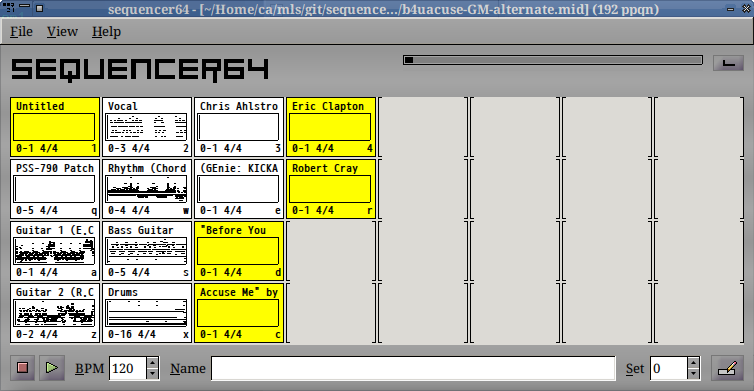
\includegraphics[scale=0.75]{seq64-first-screen.png}
%  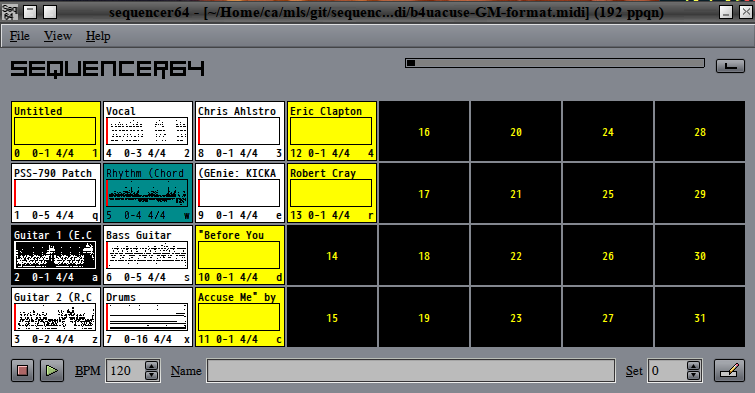
\includegraphics[scale=0.75]{new/seq64_first_screen.png}
   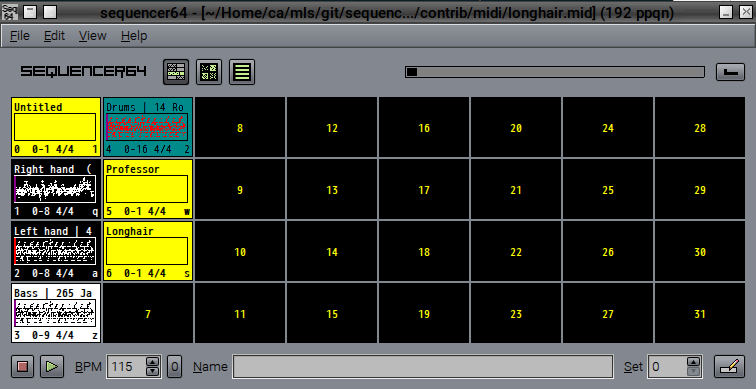
\includegraphics[scale=0.75]{seq64-first-screen-new-buttons.png}
   \caption{Sequencer64 Main Screen, 0.9.18}
   \label{fig:seq64_main_screen}
\end{figure}

   Then the \textsl{Sequencer64} main window appears, as shown in
   \figureref{fig:seq64_main_screen}.  It has some differences
   from the \textsl{Seq24} main window: the highlighting of
   empty patterns in yellow, a different font, additional control buttons,
   and much more that is not shown.
   Most of these items can be configured via the "rc" and "user" configuration
   files or command-line options.

% This Tip needs to be put elsewhere.

   \textbf{Tip:}
   \index{tips!tooltips}
   \index{tooltips}
   As with most user-interfaces, holding the mouse over any button for a
   short period will let one view a short description (tooltip)
   of what it does.

% The following "input" sections are stored in separate files of the same
% name with ".tex" appended.

\rhead{\rightmark}         % shows section number and section name

% Menu

%-------------------------------------------------------------------------------
% seq64_menu
%-------------------------------------------------------------------------------
%
% \file        seq64_menu.tex
% \library     Documents
% \author      Chris Ahlstrom
% \date        2015-08-31
% \update      2016-05-20
% \version     $Revision$
% \license     $XPC_GPL_LICENSE$
%
%     Provides the Menu section of seq24-user-manual.tex.
%
%-------------------------------------------------------------------------------

\section{Menu}
\label{sec:seq64_menu}

   The \textsl{Sequencer64} menu, as seen at the top of
   \figureref{fig:seq64_main_screen}, is fairly simple, but it is important to
   understand the structure of the menu entries.

\subsection{Menu / File}
\label{subsec:seq64_menu_file}

   The \textbf{File} menu is used to save and load standard MIDI files.
   \textsl{Sequencer64} should be able to handle any Format 1 standard files
   that any other sequencer is capable of exporting.  

   The \textsl{Sequencer64} menu entry contains the sub-items shown in
   \figureref{fig:seq64_menu_file_items}.  The next few sub-sections discuss the
   sub-items in the \textsl{File} sub-menu.

\begin{figure}[H]
   \centering 
   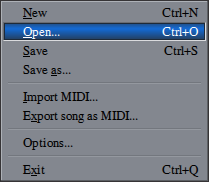
\includegraphics[scale=0.75]{menu/menu_file.png}
   \caption{Sequencer64 File Menu Items}
   \label{fig:seq64_menu_file_items}
\end{figure}

   \begin{enumber}
      \item \textbf{New}
      \item \textbf{Open...}
      \item \textbf{Save}
      \item \textbf{Save As...}
      \item \textbf{Import...}
      \item \textbf{Options...}
      \item \textbf{Exit}
   \end{enumber}

\subsection{Menu / File / New}
\label{subsec:menu_file_new}

   The \textbf{New} menu entry clears out any current song and patterns,
   allowing one to create news ones from scratch.
   If unsaved changes are pending, the user will be prompted to save the
   changes.

   \index{todo!improve change detection}
   \textsl{Currently, the detection of situations requiring a save (or not
   requiring a save) needs a bit of work.  We've made a lot of progress,
   though.}

\subsubsection{Menu / File / Open}
\label{subsubsec:seq64_menu_file_open}

   The \textbf{Open} menu entry opens a song (MIDI file)
   that had been saved previously.  It opens up a standard GTK+2 file dialog:

\begin{figure}[H]
   \centering 
   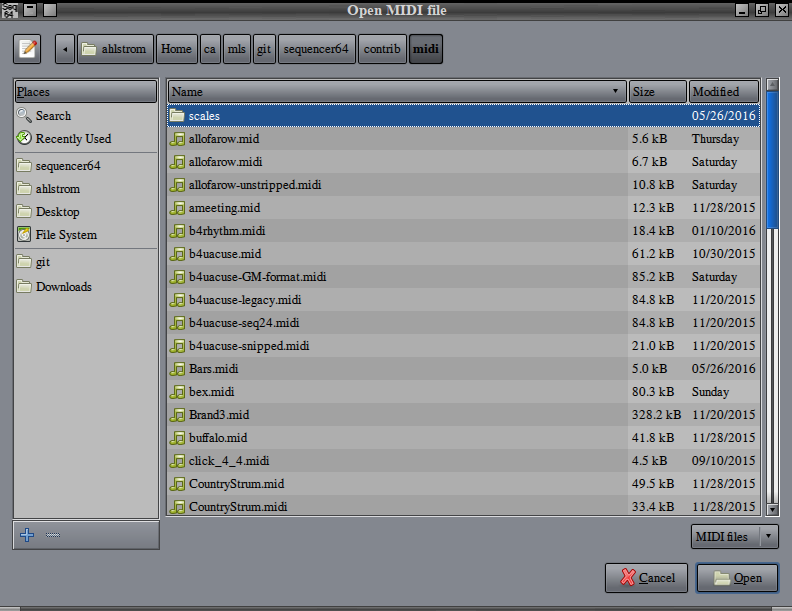
\includegraphics[scale=0.50]{menu/menu_file_open.png}
   \caption{File Open}
   \label{fig:seq64_menu_file_open}
\end{figure}

   If unsaved changes are pending, the user will (usually)
   be prompted to save the changes.
   When in doubt, save!  If still in doubt, keep backups of your tunes!

\subsubsection{Menu / File / Save and Save As}
\label{subsubsec:menu_file_open_save_as}

   The \textbf{Save} menu entry saves the song under its current file-name.
   If there is no current file-name, then it opens up a standard GTK+2 file
   dialog to name and save the file.

   The \textbf{Save As} menu entry saves a song under a different name.
   It opens up the following standard GTK+2 file dialog:

\begin{figure}[H]
   \centering 
   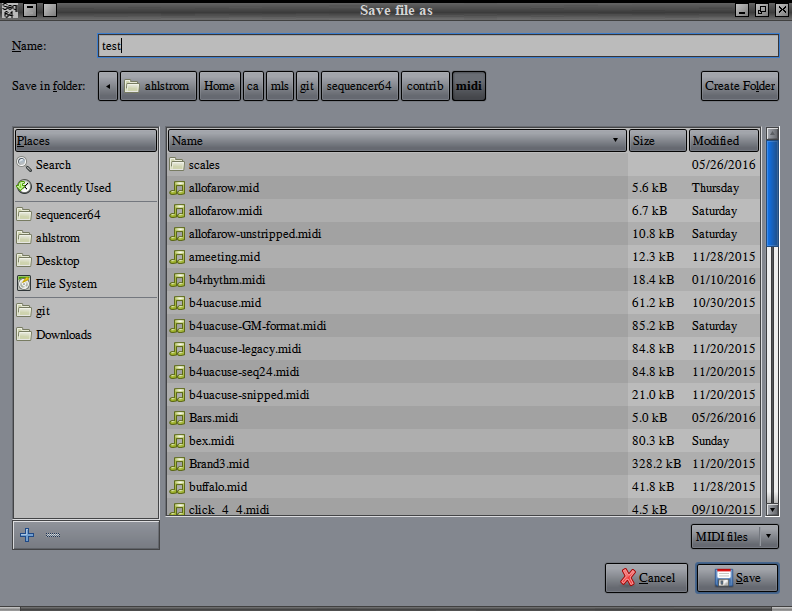
\includegraphics[scale=0.50]{menu/menu_file_save_as.png}
   \caption{File Save As}
   \label{fig:seq64_menu_file_save_as}
\end{figure}

   To save a new file, or to save the current existing file to a new name,
   enter the name in the name field, \textsl{without an extension}.
   \textsl{Sequencer64} will append a \texttt{.midi} extension to the filename.
   The file will be saved in a format that the Linux \textsl{file} command
   will tag as something like:

   \begin{verbatim}
      myfile.midi: Standard MIDI data (format 1) using 16 tracks at 1/192
   \end{verbatim}

   It looks like a simple MIDI file, and yet, if one re-opens it in
   \textsl{Sequencer64}, one sees that all of the labelling, pattern information,
   and song layout has been preserved in this file.
   Even the pattern subsections, as discussed in
   \sectionref{subsubsec:seq64_song_editor_arrangement_panel_roll},
   have been saved.
   (But the L and R marker positions are not saved.)

   Compare the sizes of the original project MIDI file,
   \texttt{contrib/b4uacuse.mid}, and the output MIDI file after
   \textsl{Sequencer64} saved the patterns and the song layout we created,
   \texttt{contrib/b4uacuse-seq24.midi}.  The latter is a lot
   bigger.

   The reason is that, after the last track in the file, a number of
   sequencer-specific (SeqSpec) items are saved, to preserve this extra
   information.  In legacy mode, \textsl{Sequencer64} saves this information
   in the same format as \textsl{Seq24}.  Unfortunately, this format is
   not quite standard, and a few MIDI applications may produce error
   messages (as opposed to just ignoring it) when parsing this section. 
   
   \textbf{New:}
   \index{new!seqspec format}
   Therefore, in its normal mode, \textsl{Sequencer64} saves this
   information in a more MIDI-compliant format, marking each SeqSpec section
   as vendor-specific information, and marking this section as a regular
   MIDI track.
   The legacy and new formats of the final "track" are explained in
   \sectionref{subsec:legacy_midi_format}.

\subsubsection{Menu / File / Import}
\label{subsubsec:seq64_menu_file_import}

   The \textbf{Import} menu entry allows one to import a Format 1 MIDI file
   into one or more patterns, one pattern per track in the MIDI file.
   Even long tracks, that aren't short loops, are read in properly.

\begin{figure}[H]
   \centering 
   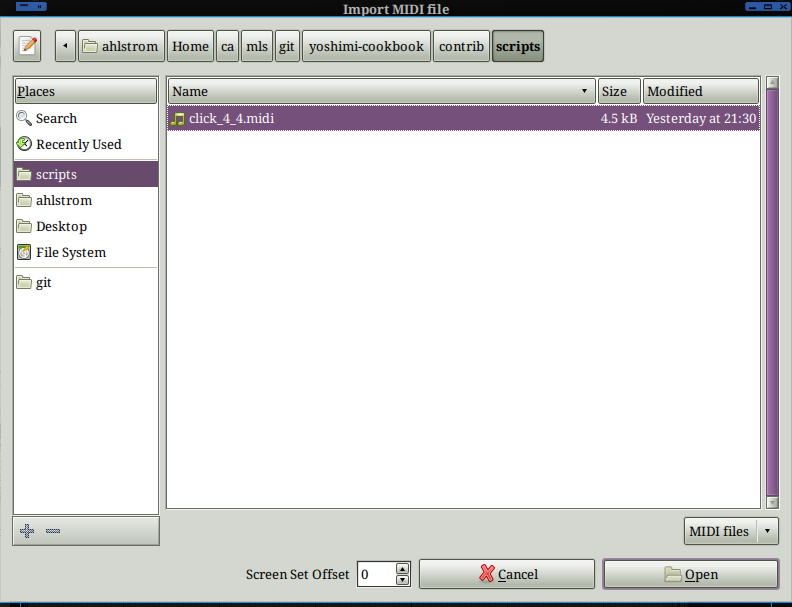
\includegraphics[scale=0.50]{menu/menu_file_import.png}
   \caption{File Import}
   \label{fig:seq64_menu_file_import}
\end{figure}

   When imported, each track, whether a music track or an information track,
   is entered into its own loop/pattern box.  The import operation can
   handle reasonably complex files, as shown in the following diagram, which
   shows an import of the \texttt{contrib/b4uacuse.mid} file, which contains
   a transcription of an Eric Clapton tune that we'd made over 20 
   years ago and had uploaded to the \textsl{GEnie} network service.

   Note the additional file-dialog field,
   \textbf{Select Screen Offset}.
   \index{import!select screen offset}
   \index{select screen offset}
   This setting lets one place the imported data into a screen-set other than
   the first screen-set, screen-set 0.
   This field is not editable.  It requires using the scroll button to move the
   screen set offset up or down in value.  The legal values range from -31 to 0
   to +31.
   
   When the file is imported, the sequence number for each track read in is
   adjusted to put the track in the desired screen set.  The negative numbers
   are probably more useful to move sequences around in an already-created
   \textsl{Sequencer64} song file with a lot of screen-sets in it.

\begin{figure}[H]
   \centering 
   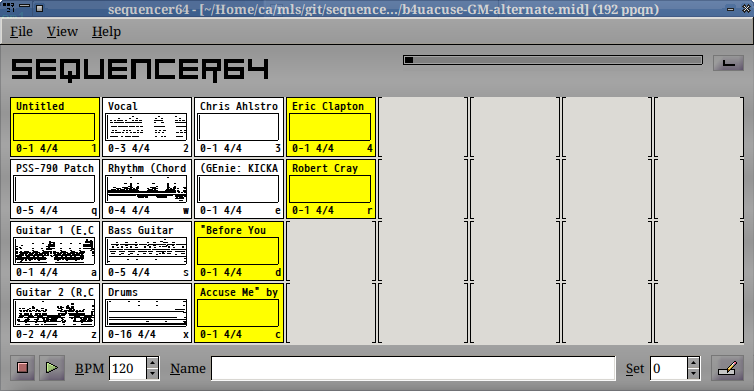
\includegraphics[scale=0.90]{menu/imported_midi_song.png}
   \caption{Imported MIDI Song}
   \label{fig:seq64_imported_midi_song}
\end{figure}

   This song has a number of non-event tracks containing labels.
   \textbf{New:}
   \index{new!empty tracks}
   These tracks are treated as "empty", and show up with a yellow
   background.  They are ignored on playback.   Some of the tracks
   which look empty, but are not yellow, contain program-change events.

   Unfortunately, this song was created before the days of General MIDI.
   It was scored for the Yamaha PSS-790 consumer-level synthesizer,
   definitely not a GM-compliant device.
   One can use the MIDI-conversion project, \textsl{midicvt}
   (see reference \cite{midicvt}),
   to convert it to General MIDI format, including General MIDI drums.

\subsubsection{Menu / File / Options}
\label{subsubsec:seq64_menu_file_options}

   The \textbf{Options} menu item provides a number of settings in one
   tabbed dialog, shown in the figures that follow.
   This dialog allows one to select which sequence gets the MIDI
   clock, which incoming MIDI events control the sequencer, what keys are
   mapped to functions, how the mouse works, and some JACK parameters.

\paragraph{Menu / File / Options / MIDI Clock}
\label{paragraph:seq64_menu_file_options_midi_clock}

   The \textbf{MIDI Clock} tab provides a way to send the MIDI clock to one
   or more of the \textsl{Sequencer64} output busses.
   It is used to configure to what busses the MIDI clock gets dumped.
   It also shows the devices that one can play music with.
   The items that appear in this tab depend on four things:

   \begin{itemize}
      \item What MIDI devices are connected to the computer.  For example,
         MIDI controllers, USB MIDI cables, and other devices will add MIDI
         output devices (ports) to the system.
      \item What MIDI software devices are running on the computer.
         For example, running MIDI software synthesizers such as
         \textsl{Timidity} and \textsl{Yoshimi} will add extra output devices
         (playback ports) to a system.
      \item The setting of the "manual ALSA ports" option,
         \texttt{--manual\_alsa\_ports} command-line option or the
         \texttt{[manual-alsa-ports]} section of the
         \texttt{sequencer64.rc} configuration file, as described in
         \sectionref{subsec:seq64_rc_file_other_midi}
      \item The setting of the \textsl{Sequencer64}-specific
         "reveal ALSA ports" option,
         \texttt{--reveal\_alsa\_ports} command-line option or the
         \texttt{[reveal-alsa-ports]} section of the
         \texttt{sequencer64.rc} configuration file, as described in
         \sectionref{subsec:seq64_rc_file_other_midi}
   \end{itemize}

   For the current discussion, a USB MIDI cable was plugged into the system,
   and the \textsl{Timidity} and \textsl{Yoshimi} (in ALSA mode) software
   synthesizers were running.  \textsl{Sequencer64} was also running, of
   course.  Here are the devices shown by the ALSA MIDI playback
   command-line application:

   \begin{verbatim}
      $ aplaymidi -l
       Port    Client name                      Port name
       14:0    Midi Through                     Midi Through Port-0
       24:0    USB2.0-MIDI                      USB2.0-MIDI MIDI 1
       24:1    USB2.0-MIDI                      USB2.0-MIDI MIDI 2
      128:0    TiMidity                         TiMidity port 0
      128:1    TiMidity                         TiMidity port 1
      128:2    TiMidity                         TiMidity port 2
      128:3    TiMidity                         TiMidity port 3
      130:16   seq24                            seq24 in
   \end{verbatim}

   (For some reason, the \textsl{Yoshimi} input port is not showing up
   in the output of \texttt{aplaymidi}, though, as shown in
   \figureref{fig:seq64_midi_clock_4_devices_manual_0},
   \textsl{Sequencer64} sees it on port 7.  Perhaps that application is not
   providing a good ALSA device name.)
   
   Turning to \figureref{fig:seq64_midi_clock_4_devices_manual_1},
   note the 16 devices provided by
   \textsl{Sequencer64}.  Also note that its first value is 1, not 0, due to
   the MIDI Thru port occupying slot 0.
   This figure shows the result with the manual ALSA option of
   \textsl{Sequencer64} turned on.

\begin{figure}[H]
   \centering 
   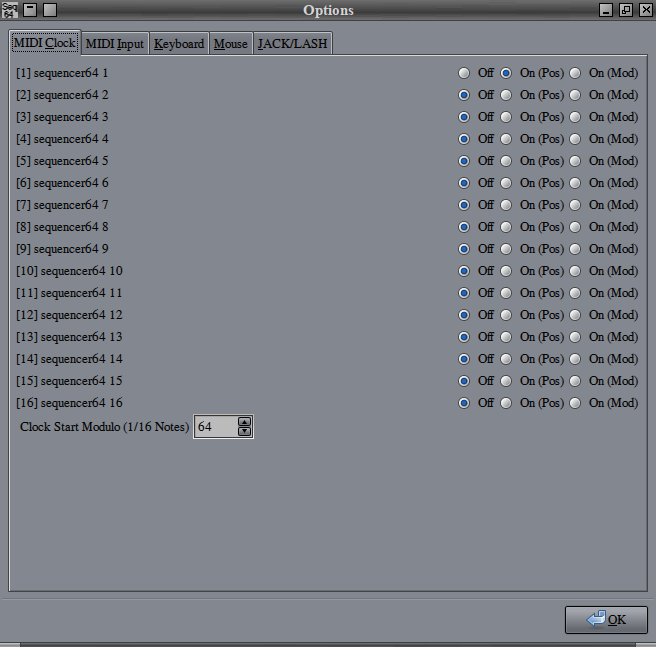
\includegraphics[scale=0.75]{menu/midi-clock-4-devices-manual-1.png}
   \caption{MIDI Clock, Manual ALSA Option On}
   \label{fig:seq64_midi_clock_4_devices_manual_1}
\end{figure}

   It basically shows the 16 MIDI output busses that \textsl{Sequencer64} can
   drive.  One would have to use an ALSA MIDI connection application to put a
   device on each of those outputs.  The fact that the the buss names can
   start with different numbers, depending on the system setup, can complicate
   the playing of MIDI in this manner.

   The following elements are present in this dialog:

   \begin{enumber}
      \item \textbf{Buss Name}
      \item \textbf{Off}
      \item \textbf{On (Pos)}
      \item \textbf{On (Mod)}
      \item \textbf{Clock Start Modulo}
   \end{enumber}

   \setcounter{ItemCounter}{0}      % Reset the ItemCounter for this list.

   \itempar{Buss Name}{midi clock!buss name}
   \index{port name}
   \index{midi clock!port name}
   These labels indicate the output busses (ports) of \textsl{Sequencer64}.
   They range from \textbf{[1] seq24 1} to \textbf{[16] seq24 16}.

   \itempar{Off}{midi clock!off}
   This setting disables the MIDI clock for the given output buss.
   However, note that MIDI output can still be sent to those ports, and
   each port that has a device connected to it will play music.
   
   For feeding \textsl{Yoshimi} with MIDI data, we found that this
   setting is the one that must be made in order for \textsl{Yoshimi} to
   produce a sound.

   \itempar{On (Pos)}{midi clock!on (pos)}
   The MIDI clock will be sent to this buss.
   MIDI Song Position and MIDI Continue will be sent if playback is starting
   at greater than tick 0 in Song mode.  Otherwise, MIDI Start will be sent.

   \itempar{On (Mod)}{midi clock!on (mod)}
   The MIDI clock will be sent to this buss.
   MIDI Start will be sent and clocking will begin
   once the Song Position has reached the start modulo of the specified size
   (see the next item's description).
   This setting is used for gear that does not respond to Song Position.

   \itempar{Clock Start Modulo}{midi clock!clock start modulo}
   Clock Start Modulo (1/16 Notes).
   This value starts at 1 and ranges on upward to 16384.
   It  defaults to 64.
   It is used by the \textbf{On (Mod)} setting discussed above.
   It is the \texttt{[midi-clock-mod-ticks]} option in the \textsl{Sequencer64}
   "rc" file as described in
   \sectionref{subsec:seq64_rc_file_other_midi}.

\begin{figure}[H]
   \centering 
   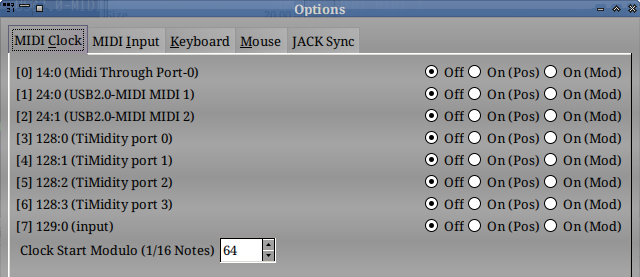
\includegraphics[scale=0.75]{menu/midi-clock-4-devices-manual-0.png}
   \caption{MIDI Clock, Manual ALSA Option Off}
   \label{fig:seq64_midi_clock_4_devices_manual_0}
\end{figure}

   As shown by the figure above, with the manual ALSA option turned off,
   all of the devices that can be driven by MIDI output are shown,
   including the MIDI Thru port, the two MIDI ports on the USB cable,
   the four ports provided by \textsl{Timidity}, and the unlabelled
   port provided by \textsl{Yoshimi}.

   One could theoretically play music through 6 or 7 devices using
   \textsl{Sequencer64} with this setup.

   \textbf{TODO:} \index{todo!manual alsa gui option}
   There is currently no user-interface item corresponding to this command-line
   and "rc" configuration file option.

\paragraph{Menu / File / Options / MIDI Input}
\label{paragraph:seq64_menu_file_options_midi_input}

   To allow \textsl{Sequencer64} to record MIDI from MIDI devices such as
   controllers and keyboards, the output of the ALSA MIDI recording
   command-line application is relevant:

   \begin{verbatim}
      $ arecordmidi -l
       Port    Client name                      Port name
       14:0    Midi Through                     Midi Through Port-0
       24:0    USB2.0-MIDI                      USB2.0-MIDI MIDI 1
      130:0    seq24                            [1] seq24 1
      130:1    seq24                            [2] seq24 2
      130:2    seq24                            [3] seq24 3
       . . .   . . .                               . . .
      130:15   seq24                            [16] seq24 16
   \end{verbatim}

   We see that we can record MIDI from the MIDI Thru port, from the USB MIDI
   cable, and MIDI from any of the 16 output ports provided by the manual ALSA
   port mode of \textsl{Sequencer64}.

   If the "manual ALSA ports" option (see below) is turned on,
   then the only item in the \textbf{MIDI Input} tab is the single MIDI input
   buss provided by \textsl{Sequencer64}:  \textbf{[0] seq24 0}, or, since
   the MIDI Thru port takes slot 0, \textbf{[1] seq24 1}.

\begin{figure}[H]
   \centering 
   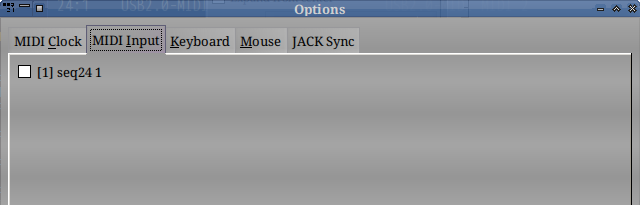
\includegraphics[scale=0.75]{menu/midi-input-4-devices-manual-1.png}
   \caption{MIDI Input, Manual ALSA Ports On}
   \label{fig:seq64_midi_input_4_devices_manual_1}
\end{figure}

   This item, if checked, allows \textsl{Sequencer64} to be used to record MIDI
   information from another source (which must be connected to this port by
   another application), or pass it through to the output busses
   that are configured to allow pass-through
   (in the Pattern Editor, as discussed in 
   \sectionref{subsec:seq64_pattern_editor_bottom}.)

   If the "manual ALSA ports" option is turned off, then
   the input ports from the system are shown:

\begin{figure}[H]
   \centering 
   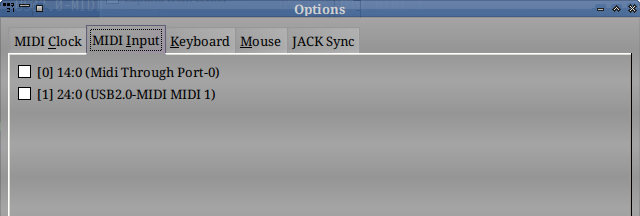
\includegraphics[scale=0.75]{menu/midi-input-4-devices-manual-0.png}
   \caption{MIDI Input, Manual ALSA Ports Off}
   \label{fig:seq64_midi_input_4_devices_manual_0}
\end{figure}

   For example, one could check input \#1 to have \textsl{Sequencer64} record
   MIDI from an old-fashioned MIDI keyboard that is connected to the USB MIDI
   cable.  If the keyboard didn't have a sound generator, one would also want
   \textsl{Sequencer64} to pass this MIDI on to a sound generator, such as a
   software or hardware synthesizer attached to one of the ports shown in
   \figureref{fig:seq64_midi_clock_4_devices_manual_0}.

\paragraph{Menu / File / Options / Keyboard }
\label{paragraph:seq64_menu_file_options_keyboard}

   \textsl{Seq24}, as befits a good application, allows extensive use of
   keyboard shortcuts to make operations go faster than when using a mouse,
   and \textsl{Sequencer64} continues that tradition.
   The \textbf{Keyboard} tab allows for the configuration of these keyboard
   shortcuts.

   \textbf{Warning:}
   Whenever one of the text fields in this dialog has the focus (and that is
   usually the case), then any keystroke, including keys like Ctrl, Alt,
   and Super (Mod4 or Windows key), can alter the value of a field to that
   of the keystroke.  This change is very easy to do accidentally!
   \textbf{Use the mouse}
   to move this window and to click its \textbf{OK} button!

\begin{figure}[H]
   \centering 
   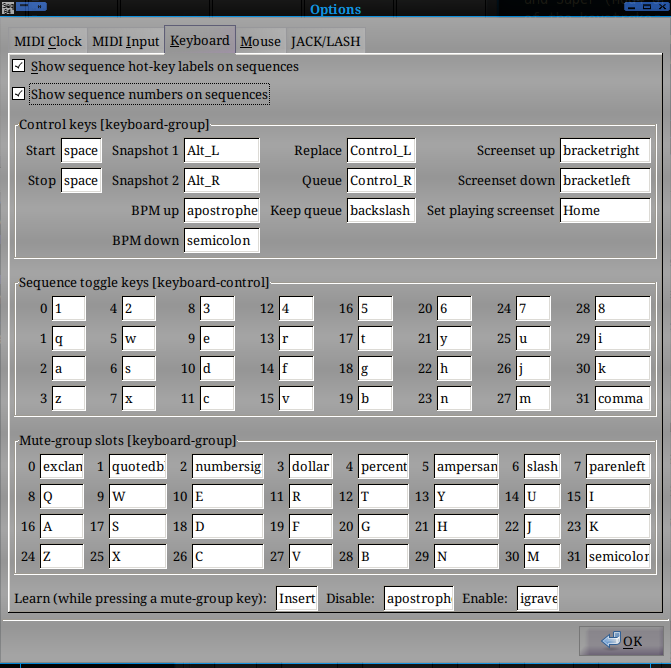
\includegraphics[scale=0.75]{menu/menu_file_options_keyboard.png}
   \caption{File / Options / Keyboard}
   \label{fig:seq64_menu_file_options_keyboard}
\end{figure}

   We won't attempt to cover every user-interface item in this busy
   dialog, just the categories.  Some items are discussed in other parts of
   this manual.

   \textbf{New:}
   \index{new!pause}
   \index{pause}
   Also, if the application has been built with the pause option, an
   additional key definition is shown, as in the following figure:

\begin{figure}[H]
   \centering 
   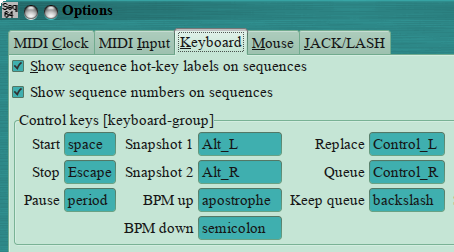
\includegraphics[scale=0.75]{new/keyboard-options-0_9_10_1.png}
   \caption{File / Options / Keyboard, with Pause}
   \label{fig:seq64_menu_file_options_keyboard_pause}
\end{figure}

   By default, the Pause key is the period (".").  An old version of
   the "rc" file is automatically fixed to include this new option.
   The pause feature can be removed by rebuilding the application
   after configuring with the \texttt{--disable-pause} option.

   To continue with a listing of the keyboard options:

   \begin{enumber}
      \item \textbf{Show key labels on sequences}
      \item \textbf{Show sequence numbers on sequences}
      \item \textbf{Control keys}
      \item \textbf{Sequence toggle keys}
      \item \textbf{Mute-group slots}
      \item \textbf{Learn}
      \item \textbf{Disable}
      \item \textbf{Enable}
   \end{enumber}

   \setcounter{ItemCounter}{0}      % Reset the ItemCounter for this list.

   \itempar{Show key labels on sequence}{keyboard!show labels}
   This item, if enabled, shows the key labels in the lower-right corner of
   each loop/pattern in the Patterns window (the main window).  This feature is
   useful for live playback and control of a song.
   Note that this option is also available in the "rc" configuration file.

   \itempar{Show sequence numbers on sequence}{keyboard!sequence numbers}
   \textbf{New:}
   \index{new!sequence numbers}
   If this option is turned on, the
   empty slots in the Patterns window show the prospective sequence number.
   See the following figure for the look.

\begin{figure}[H]
   \centering 
   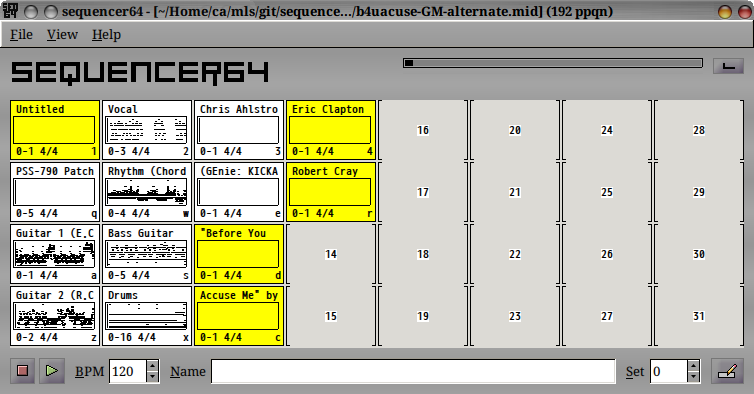
\includegraphics[scale=0.75]{pattern-window-with-numbering.png}
   \caption{Pattern Window with Numbering}
   \label{fig:seq64_build_with_numbering}
\end{figure}

   If you don't like it, turn off the option, or try other grid options
   in the "user" configuration file.

   Also note that this option also changes the visibility of sequence numbers
   in active sequences and in the performance editor's names column.

   \itempar{Control keys}{keyboard!control keys}
   This block of fields provides shortcut keys for many operations of
   \textsl{Sequencer64}.

   \begin{enumber}
      \item \textbf{Start}.
         Key: \index{keys!space} \textbf{space}.
      \item \textbf{Stop}.
         Key: \index{keys!esc} \textbf{Escape}.
      \item \textbf{Pause}. (new)
         Key: \index{keys!period} \textbf{period}.
      \item \textbf{Snapshot 1}.
         Key: \index{keys!alt-l} \textbf{Alt\_L}.
      \item \textbf{Snapshot 2}.
         Key: \index{keys!alt-r} \textbf{Alt\_R}.
      \item \textbf{bpm up}.
         Key: \index{keys!apostrophe} \textbf{apostrophe}.
      \item \textbf{bpm down}.
         Key: \index{keys!semicolon} \textbf{semicolon}.
      \item \textbf{Replace}.
         Key: \index{keys!ctrl-l} \textbf{Control\_L}.
      \item \textbf{Queue}.
         Key: \index{keys!ctrl-r} \textbf{Control\_R}.
      \item \textbf{Keep queue}.
         Key: \index{keys!backslash} \textbf{backslash}.
      \item \textbf{Screenset down}.
         Key: \index{keys![} \textbf{bracketleft}.
      \item \textbf{Screenset up}.
         Key: \index{keys!]} \textbf{bracketright}.
      \item \textbf{Set playing screenset}.
         Key: \index{keys!home} \textbf{Home}.
   \end{enumber}

   Note that some of the keys have positional mnemonic value.  For example,
   for BPM control, the semicolon is at the left (down), and the apostrophe
   is at the right (up).

   Also note that the keys definable in this tab are only a subset of the
   various keys that can be used, especially keys used with the
   \texttt{Ctrl} key or other modifier keys.

   \index{snapshot}
   A \textsl{snapshot} is a briefly preserved state of the patterns.
   One can press a snapshot key, change the state of the patterns for live
   playback, and then release the snapshot key to revert to the state when
   the snapshot key was first pressed.

   \index{queue}
   To "queue" a pattern means to ready it for playback upon the next repeat
   of a pattern.  A pattern can be armed immediately, or it can be queued to
   play back the next time the pattern starts.
   A pattern can be queued by holding the queue key (defined in
   \textbf{File / Options / Keyboard / queue}) and pressing a pattern-slot
   shortcut key.  Instead of the pattern turning on immediately, it turns on at
   the next repeat of the pattern.

   \index{keep queue}
   \index{queue!keep}
   The "keep queue" functionality allows the queue to be held without holding
   down the queue button the whole time.  First, press the keep-queue key
   (defined in \textbf{File / Options / Keyboard / Keep queue}).  Now, hitting
   any of the shortcut keys, no matter how many, sets up the corresponding
   pattern slot to be queued.  This mode is disabled by hitting the
   "queue" key (any currently active queues remain active until finished).

   \itempar{Sequence toggle keys}{keyboard!sequence toggle keys}
   Each of these keys toggles the playing/muting of one of the 32
   loop/pattern boxes.  These keys are layed out logically on the keyboard,
   and can also be shown in each loop/pattern box.  No need to list them all
   here!  Please note that we often call them "shortcut keys" where the context
   makes it clear that they apply to the armed/unarmed state of a pattern.

   \itempar{Mute-group slots}{keyboard!mute-group slots}
   Each of these keys operates on the mute-grouping of one of the 32
   loop/pattern boxes.  These keys are layed out logically on the keyboard,
   and can also be shown in each loop/pattern box.  No need to list them all
   here!

   \index{todo!mute-group}
   One thing we need to discover is just what this mute-grouping
   means functionally.
   Apparently groups work with the playing screen set only.
   Change the screenset and give the command to make it the playing one
   (e.g. set the HOME key for this purpose.)

   \itempar{Learn}{keyboard!learn}
   Learn (while pressing a mute-group key).
   This items sets the key used to initiate a learn mode.
   It is the \textbf{Insert} key by default.

   \itempar{Disable}{keyboard!disable}
   \textbf{TODO:} \index{todo!keyboard disable} What gets disabled?
   \index{keys!apostrophe}
   It is the \textbf{apostrophe} key by default.

   \itempar{Enable}{keyboard!enable}
   \textbf{TODO:} What gets enabled?
   \index{keys!igrave}
   It is the \textbf{igrave} (back-tick) key by default.

   There is much to learn about this learn/enable/disable triad!

\paragraph{Menu / File / Options / Mouse }
\label{paragraph:seq64_menu_file_options_mouse}

   This item selects the mouse-interaction method.

\begin{figure}[H]
   \centering 
   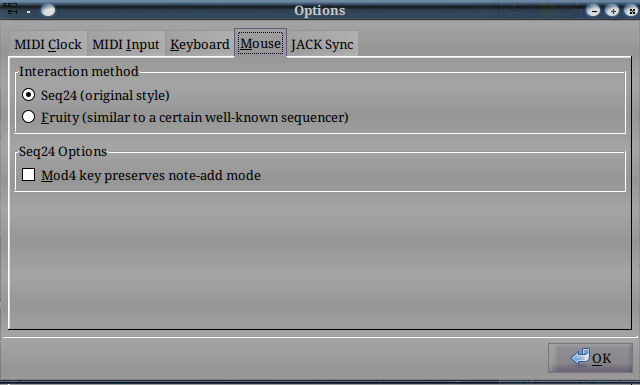
\includegraphics[scale=0.75]{menu/menu_file_options_mouse_condensed.png}
   \caption{File / Options / Mouse (Condensed View)}
   \label{fig:seq64_menu_file_options_mouse}
\end{figure}

   The default method is \textbf{seq24 (original style)}.
   The alternate method is \textbf{fruity (similar to a certain well known
   sequencer)}.

   \index{mouse!fruity}
   The alternate method is presumably that of the \textsl{Fruity Loops}
   (now \textsl{FL Studio}) sequencer.  The fruity mode seems to involve the
   following (based on scanning the source code):
   
   \begin{itemize}
      \item \textbf{Left-click left side}.
         Begin a grow/shrink operation for the left side.
      \item \textbf{Left-click right side}.
         Begin a grow/shrink operation for the right side.
      \item \textbf{Left-click middle}.
         Move the object.
      \item \textbf{Left-click}.
         Add an event if nothing selected.
      \item \textbf{Middle-click}.
         Split the note?
   \end{itemize}

   The \textsl{Seq24} "original style" is pretty much as expected for basic
   actions such as selecting and moving notes using the left mouse button.
   Drawing a note or event is a bit different, in the one must first
   \textsl{click and hold} the right mouse button, and then
   \textsl{click and drag} the right mouse button to insert notes,
   Notes are inserted to be at the current length and grid-snap values for
   the sequence editor for as long as the left button is pressed.
   Notes are inserted only up to the boundary of the sequence length.
   And, once notes are inserted, moving the mouse with the left button still
   held down simply moves the notes to the new note value of the mouse.

   If one releases the left button, then presses and holds it again,
   more notes will be added in the same way.
   This is strange, but it is a powerful way to layer notes into a short
   sequence.
   We call it the \index{draw mode} \index{mode!draw } "draw mode" or
   \index{paint mode} \index{mode!paint } "paint mode".

   Note that drawing/painting can also be done while the sequence is playing,
   and notes will be added to be played the next time the progress bar crosses
   them.
   
   \textbf{New:}
   \index{new!Mod4 mode}
   \index{keys!Mod4}
   \label{new_mod4_mode}
   \textbf{The Mod4 Right-Click Mode}.
   In order to work better with certain trackpads, the
   "Seq24" mode of mouse interaction can be modified (only in the
   Pattern Editor at present) so that the Mod4 key (Super or Windows key)
   can be pressed when releasing the right mouse button.
   This keeps the mouse in note-add mode.
   Another right-click, without pressing Mod4, will exit this mode.

   The reason for this feature is the crummy FocalTech touchpad on one of
   the author's laptops.  This trackpad seems to have only a single button,
   which the driver interprets as left or right depending where the finger
   is when it is clicked.  There's no way to click the right and left
   buttons at the same time.  There's no way to make a middle-click action.

   Note that this option will not interfere with the Mod4 key being set
   in the \textbf{Keyboard} option tab, since the keys there mainly apply to
   the Patterns Panel (main window).

% Move this section to the right place and simply create a section-reference to
% it here.

   \textbf{New:}
   \index{new!paint mode}
   Another way to turn on the paint mode has been added, based on a feature
   found in a patch that someone posted about in some mailing list somewhere on
   the internet.
   To turn on the paint mode, press the
   \index{keys!p}
   "p" key while in the sequence editor.
   This is just like pressing the right mouse button, but the draw/paint mode
   sticks (as if the Mod4 mode were in force).
   To get out of the paint mode, press the
   \index{keys!x}
   "x" key while in the sequence editor.
   These keys, however, do not work (currently) while the sequence is playing.

   \index{todo:extend mouse support}
   \textbf{TODO:} These convenience options are currently limited to the
   pattern/sequence editor window and the performance editor window, and may
   need some heavier testing.  But note that some \textsl{Sequencer64} windows
   can use the ctrl-left-click as a middle click. 
 
\paragraph{Menu / File / Options / Jack Sync and LASH}
\label{paragraph:seq64_menu_file_options_jack_sync}

   This tab sets up options for JACK synchronization, if \textsl{Sequencer64}
   was built with JACK support.  (Why wouldn't it be?)
   This tab also sets up options for using LASH session management, if
   \textsl{Sequencer64} was build with LASH support.

\begin{figure}[H]
   \centering 
   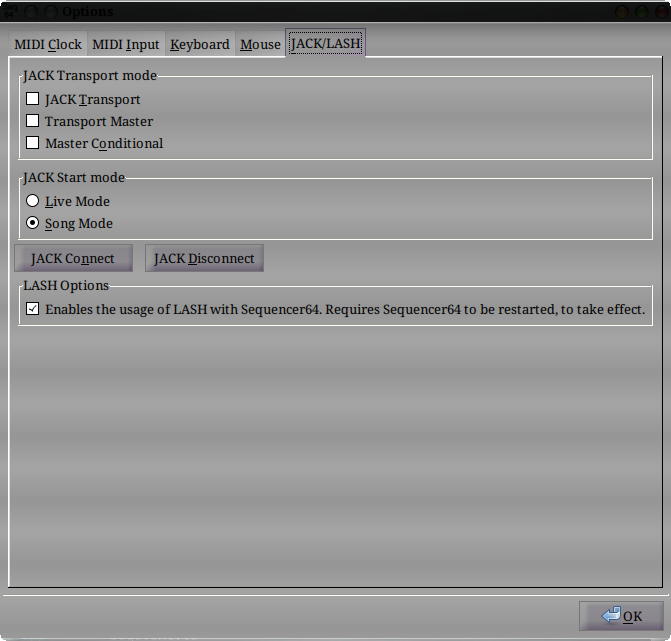
\includegraphics[scale=0.75]{menu/menu_file_options_jack_sync.png}
   \caption{File / Options / JACK Sync or JACK/LASH}
   \label{fig:seq64_menu_file_options_jack_sync}
\end{figure}

   \begin{enumber}
      \item \textbf{Transport}
      \item \textbf{JACK Start mode}
      \item \textbf{Connect}
      \item \textbf{Disconnect}
      \item \textbf{LASH Options}
   \end{enumber}

   \setcounter{ItemCounter}{0}      % Reset the ItemCounter for this list.

   \itempar{Transport}{jack sync!transport}
   These settings are stored in the "rc" file settings group
   \texttt{[jack-transport]}.
   See \sectionref{subsec:seq64_rc_file_jack_transport},
   which describes this configuration option.
   This items collects the following settings:

   \begin{itemize}
      \item \textbf{Jack Transport}.
         \index{JACK!transport}
         Enables slave synchronization with JACK Transport.
         The command-line option is \texttt{--jack\_transport}.
         The behavior of this mode of operation is perhaps not quite
         correct.  Even as a slave, \textsl{Sequencer64} can start and
         stop playback.
      \item \textbf{Transport Master}.
         \index{JACK!transport master}
         \textsl{Sequencer64} will attempt to serve as the JACK Master.
         The command-line option is \texttt{--jack\_master}.
      \item \textbf{Master Conditional}.
         \index{JACK!master conditional}
         \textsl{Sequencer64} will fail to serve as the JACK Master if there is
         already a Master set.
         The command-line option is \texttt{--jack\_master\_cond}.
   \end{itemize}

   Note that there are long-standing issues with the JACK support of
   \textsl{Seq24}, and \textsl{Sequencer64} currently inherits some of them,
   in spite of some bug fixes.  Generally, if one experiences issues in
   transport control, try making one of the other sequencer applications the
   JACK Master.

   Also be aware that, if one starts \textsl{Sequencer64} without JACK running,
   it will take a little while for \textsl{Sequencer64} to start up.

   Finally, if one makes a change in the JACK settings, it is best to
   then press the \textbf{Disconnect} button, then the \textbf{Connect}
   button.  Another option is to restart \textsl{Sequencer64}... the settings
   are automatically saved when \textsl{Sequencer64} exits.

   \itempar{JACK Start mode}{jack sync!start mode}
   This item collects the following settings, also stored in the "rc" file
   settings group \texttt{[jack-transport]}.

   \begin{itemize}
      \item \textbf{Live Mode}.
         \index{JACK!live mode}
         \index{live mode}
         \index{non-playback mode}
         Playback will be in live mode.  Use this option to allow muting and
         unmuting of patterns.  This option might also be called "non-playback
         mode".
         The command-line option is \texttt{--jack\_start\_mode 0}.
      \item \textbf{Song Mode}.
         \index{JACK!song mode}
         \index{song mode}
         \index{playback mode}
         \index{performance mode}
         Playback will use only the Song Editor's data.
         The command-line option is \texttt{--jack\_start\_mode 1}.
   \end{itemize}

   Note that, in ALSA mode (non-JACK mode), \textsl{Sequencer64} 
   now \textsl{does} select the playback modes
   according to which window started the playback.
   We have reverted back to legacy \textsl{Seq24} behavior.
   
   \textsl{The main window, or pattern
   window, causes playback to be in live mode.  The user can arm and mute
   patterns in that windows, by clicking on sequences, using their hot-keys,
   and by using the group-mode and learn-mode features (we think).
   The song editor causes playback to be in performance mode, also known as
   "playback mode", or "song mode".}

   Of course, in JACK mode,
   it selects them according to the chosen live/song mode as discussed above.

   \itempar{Connect}{jack sync!connect}
   Connect to JACK Sync.

   \itempar{Disconnect}{jack sync!disconnect}
   Disconnect from JACK Sync.

   \itempar{LASH Options}{lash!option}
   Currently contains only one item, which enables the usage of LASH session
   management.
   Currently, \textsl{Sequencer64} needs to be restarted to complete the
   enabling or disabling of LASH support.
   Like the rest of the options, this one is written to the "rc" configuration
   file.

\subsection{Menu / View}
\label{subsec:seq64_menu_view}

   If the "allow two perfedits" option is turned off in the "user"
   configuration file, this menu item has only one entry, \textbf{Song Editor}, 
   which is already covered by a button at the bottom of the Patterns
   window.  Selecting this item bring up the Song Editor window.
   See \figureref{fig:song_editor_window}

   The Song Editor window can also be brought up via the
   \index{song editor!ctrl-e}
   \index{keys!ctrl-e}
   Ctrl-E key.

   If the "allow two perfedits" option is turned on in the "user"
   configuration file, this menu item has two entries, as shown in the
   following figure:

\begin{figure}[H]
   \centering 
   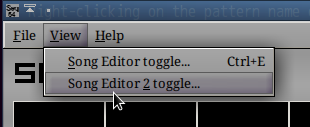
\includegraphics[scale=0.75]{menu/menu_view-dual-song-editors.png}
   \caption{Dual Song Editor Entries in View Menu}
   \label{fig:seq64_menu_view_song_editors}
\end{figure}

   Note that only the first Song Editor has a user-interface button and
   a hot-key.  Also note that there can be issues bringing up the second
   song-editor with the hot-key.  The menu entry will always work.

   If two song editors are up, they each track any changes made in the other
   song editor.  But the main purpose of two song editors is to arrange two
   different parts of the performance at the same time.

\subsection{Menu / Help About...}
\label{subsec:seq64_menu_about}

   This menu entry shows the "About" dialog.

\begin{figure}[H]
   \centering 
   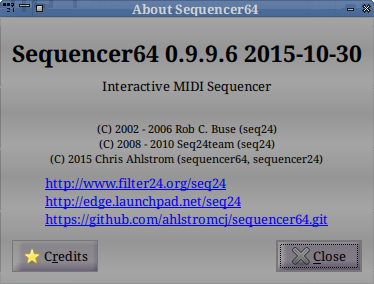
\includegraphics[scale=0.75]{menu/menu_help_about.png}
   \caption{Help About}
   \label{fig:seq64_menu_help_about}
\end{figure}

   That dialog provides access to the credits for the program, including the
   authors and the project documentors.

\begin{figure}[H]
   \centering 
   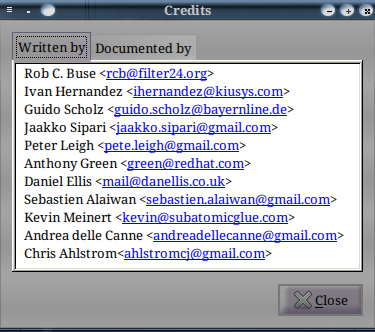
\includegraphics[scale=0.75]{menu/menu_help_credits.png}
   \caption{Help Credits}
   \label{fig:seq64_menu_help_credits}
\end{figure}

   Shows who has worked on the program, with the original author at the top
   of the list.

\begin{figure}[H]
   \centering 
   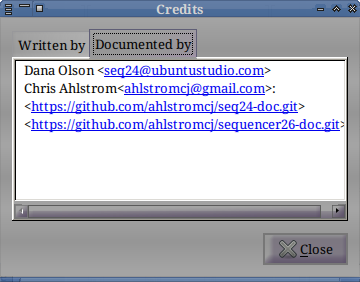
\includegraphics[scale=0.75]{menu/menu_help_doc.png}
   \caption{Help Documentation}
   \label{fig:seq64_menu_help_doc}
\end{figure}

   Shows who has documented this project.

%-------------------------------------------------------------------------------
% vim: ts=3 sw=3 et ft=tex
%-------------------------------------------------------------------------------


% Patterns Panel

%-------------------------------------------------------------------------------
% seq64_patterns_panel
%-------------------------------------------------------------------------------
%
% \file        seq64_patterns_panel.tex
% \library     Documents
% \author      Chris Ahlstrom
% \date        2015-08-31
% \update      2016-01-02
% \version     $Revision$
% \license     $XPC_GPL_LICENSE$
%
%     Provides the concepts.
%
%-------------------------------------------------------------------------------

\section{Patterns Panel}
\label{sec:seq64_patterns_panel}

   \textsl{Sequencer64} works with the idea of patterns (loops) that are
   repeated all along a song.  One composes and edits small patterns, and
   combines them to create a full song.  This is a powerful way to work, and
   makes one productive within an hour.

   The \textsl{Sequencer64 Patterns Panel} is the main window of
   \textsl{Sequencer64}.
   See \figureref{fig:seq64_main_screen}.
   It is also called the "main window" or the "patterns window".
   It is here one manages a set of patterns
   (see \sectionref{subsubsec:concepts_terms_screen_set}),
   manages the configuration, and opens the pattern or song editors.

   \index{live mode}
   When the Patterns Panel has the application focus, it puts
   \textsl{Sequencer64} in "live mode".  The musician can
   control the playback and muting/unmuting of the song, while it is
   playing, from within this window.

   For exposition, we break the Patterns Panel
   into a menu bar, a top panel, a pattern panel, and a
   bottom panel.  Note that the \textsl{Sequencer64} menu bar was
   already discussed in
   \sectionref{sec:seq64_menu}.

\subsection{Patterns / Top Panel}
\label{subsec:seq64_patterns_panel_top}

   The top panel of the Pattern window is simple, consisting of the name of
   the program and a couple of controls.

\begin{figure}[H]
   \centering 
   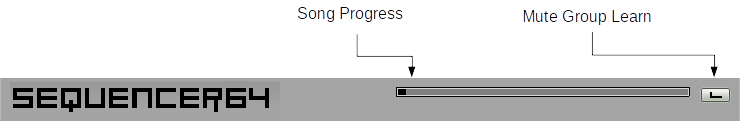
\includegraphics[scale=0.75]{pattern-window-top-panel-items.png}
   \caption{Patterns Panel, Top Panel Items}
   \label{fig:pattern_window_top_panel_items}
\end{figure}

   \begin{enumber}
      \item \textbf{Song Progress}
      \item \textbf{Mute Group Learn}
   \end{enumber}

   \setcounter{ItemCounter}{0}      % Reset the ItemCounter for this list.

   \itempar{Song Progress}{pattern!progress}
   \index{song!progress}
   \index{song!"main time"}
   The \textbf{Song Progress} bar is also known as the "main time" bar.
   This bar shows a number of small black cursors ("pills") that show the
   progress of the song through the various patterns.  For short patterns,
   the progress is fast.  For patterns that last longer, the progress is
   slow.  The whole field flashes in time with the beat.
   This field shows that something is going on.  It can also indicate
   the relative lengths of the various patterns.
 
   Note that the individual pattern boxes in the main panel, for
   patterns that are not empty, have their own
   moving progress cursor, a tall thin line in each box.

   \itempar{Mute Group Learn}{pattern!mute group learn}
   \index{"L" button}
   This button is also known as the "L" button.
   Click this button, and then press a mute-group key
   to store the mute-state of the patterns with in that key.

   See the \textbf{File / Options / Keyboard} menu entry to bring up the
   dialog showing the available mute-group keys and the corresponding
   hot-key for the "L" button.

   Group-learn is a modifier key to be pressed \textsl{together}
   with the toggle key, and the group on/off keys are there to enable/disable
   the whole feature, \textsl{not} to toggle group states.

   To set up the mute groups, press the 'L' button, and then press a key on
   the keyboard to 'learn' or 'save' the preset. Looking at the list of keys
   assigned for these mute groups (in \textbf{File / Options / Keyboard}),
   the first bank of keys are "!", "'", "?", etc., and the second bank are
   "Q", "W" "E", etc.  When you ask the program to 'learn' the key, one can't
   use the Shift key, so (on Windows at least) one cannot use the "!" or
   other symbol keys.  Similarly, make sure Caps Lock is off before starting
   the 'learn' process (as it won't recognise "q", only "Q").

   Once that works, one can configure the MIDI settings in similar ways
   by assigning MIDI commands to toggle loops, using 
   \index{rc file}
   the 'on' option in the "rc" file.
   See \sectionref{subsec:seq64_rc_file_midi_control}.

   \index{group!toggle}
	One can toggle the playing status of up to 32 previously
	defined mute/unmute patterns (groups) in the active screen
	set, similar to hardware sequencers.
   One can mute-unmute (according to the group definition) all loops in the
   playing screen set, which is the only one that can have sequences playing
   (like a live sequencer).

	This toggling is done either by one of the \textsl{group toggle} keys
	or by a MIDI controller, both assigned in the
   \index{rc file}
   \texttt{~/.config/sequencer64/sequencer64.rc} or \texttt{~/.seq24rc} files.

	A mute/unmute pattern (group) is stored by holding a
   \index{group!learn}
   \textsl{group learn} key (\texttt{Insert} by default) while pressing the
   corresponding \textsl{group toggle} key.
	There are also keys assigned to turn on/off the group functionality.

   Remember that groups work with the playing screen set only.
   One must change the screenset and give it the command to make it the
   playing one
   \index{keys!Home}
   (some set the Home key for this purpose).
   \index{rc file}
   Everything is configurable in the "rc" file.

\subsection{Patterns / Main Panel}
\label{subsec:seq64_patterns_panel_main}

   The main panel of the Patterns window provides a grid of empty boxes,
   each box delimited by brace-like lines at left and right.
   Each filled box represents a loop or pattern.
   One sees only 32 loops at a time in the main panel (but many more than
   32 loops can be supported by \textsl{Sequencer64}).
   \index{screen set}
   This group of 32 loops is called a "screen set", as discussed in
   \sectionref{subsubsec:concepts_terms_screen_set}.
   One can switch between sets by using the
   \index{keys![}
   \texttt{[} and
   \index{keys!]}
   \texttt{]} keys on the keyboard, or by using
   the spin-widget-driven, labelled \textbf{Set} interface item, or
   \index{keys!Home}
   by hitting the (default) Home key to make it the playing screenset.
   There are a total of 32 sets, for a total of 1024 loops/patterns. 
   Only one screen set can be playing at a time, according to other notes we
   have found.

\begin{figure}[H]
   \centering 
   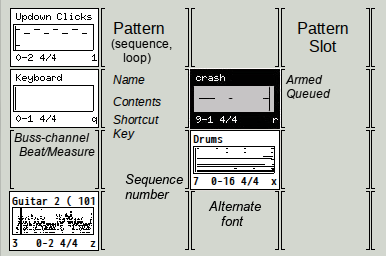
\includegraphics[scale=0.75]{pattern-window-main-panel-items.png}
   \caption{Patterns Panel, Main Panel Items}
   \label{fig:pattern_window_main_panel_items}
\end{figure}

   The individual items annoted in this figure are described in
   \sectionref{subsubsec:seq64_patterns_pattern_filled}, in more detail.

   \begin{enumber}
      \item \textbf{Pattern Slot}
      \item \textbf{Pattern}
   \end{enumber}

\subsubsection{Pattern Slot}
\label{subsubsec:seq64_patterns_pattern_slot}

   \index{pattern!slot}
   An empty box is a slot for a pattern.
   \index{pattern!right click}
   \index{slot!empty slot right-click}
   By right-clicking on an empty box one brings up a menu to create
   a new loop, as well as some other operations:

\begin{figure}[H]
   \centering 
   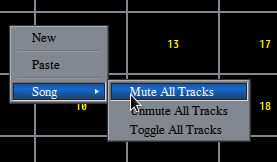
\includegraphics[scale=0.75]{pattern/pattern-empty-right-click-menu.png}
   \caption{Empty Pattern, Right-Click Menu}
   \label{fig:pattern_window_empty_right_click}
\end{figure}

   \begin{enumber}
      \item \textbf{New}
      \item \textbf{Paste}
      \item \textbf{Song / Mute All Tracks}
   \end{enumber}

   \setcounter{ItemCounter}{0}      % Reset the ItemCounter for this list.

   \itempar{New}{pattern!new}
   Creates a new loop or pattern.
   Clicking this menu entry fills in the empty box with an untitled
   pattern, and brings up the Pattern Editor
   so that one can fill in the new pattern.

   \textbf{New:}
   In addition to right-clicking and selecting \textbf{New}, the user
   \index{new!empty slot ctrl-left-click}
   can Ctrl-left-click on the empty slot, or
   \index{new!empty slot double-click}
   double-click on the empty slot, to bring up a new instance of the sequence
   editor.  For the double-click, the effect can be a bit confusing at first,
   because it currently also toggles the arming/mute status of the slot
   twice (leaving it as it was), as well.  For now, get used to it.

   \itempar{Paste}{pattern!paste}
   Pastes a loop or pattern that was previously copied.

   \itempar{Song / Mute All Tracks}{pattern!mute all}
   This item is the one item in the \textbf{Song} context menu;
   it mutes all tracks (or loops/patterns).
   It works when one has opened the Song Editor window
   and started playing in playback
   mode by starting play using that window.

   So, let us assume the song is running in playback mode.  The patterns that
   are active (unmuted) in by that playback window are shown with a black
   background in the main patterns window.  If one right clicks on a pattern
   cell and selects \textbf{Song / Mute All Tracks}, all those patterns
   will become white and be silenced.  Eventually, the Song Editor window
   catches up and shows the "M" activated for all tracks.
   
\subsubsection{Pattern}
\label{subsubsec:seq64_patterns_pattern_filled}

   A filled pattern slot is referred to informally as a pattern.
   A pattern is shown in the Pattern windows as a filled box with the
   following items of information in it.
   Examine \figureref{fig:pattern_window_main_panel_items}; it shows
   these items annotated for clarity.

   \begin{itemize}
      \item \textbf{Name}.
         \index{pattern!name}
         This line contains the name or title of the pattern, to help
         reference it when juggling a number of patters.
      \item \textbf{Contents}.
         \index{pattern!contents}
         The contents of the pattern provide a fairly detailed and
         distinguishable representation of the notes or events in the
         pattern.  Also, when the song is playing, a vertical bar cursor
         tracks the position of the playback of the pattern or loop; it
         returns to the beginning of the box every time that pattern starts
         over again.
         \textbf{New:}
         \index{new!empty pattern}
         With \textsl{Sequencer64}, an imported empty pattern will no longer
         needlessly scroll.
         However, if a pattern has even a single event (say, a program change),
         it will scroll.
         \textbf{TODO:}
         \index{todo:one-shot pattern}
         It might be good to have some patterns marked as one-shot patterns.
         They play once at the start of playback, and that is it.
         They could be marked with a cyan background.
      \item \textbf{Bus-Channel}.
         \index{pattern!bus-channel}
         This pair of numbers shows the the MIDI buss number, a dash, and
         the MIDI channel number.
         For example, "0-2" means MIDI buss 0, channel 2.
      \item \textbf{Beat}.
         \index{pattern!beat}
         This pair of numbers is the standard time-signature of the pattern,
         such as "4/4" or "3/4".  The first number is the beats-per-measure,
         and the second is the size of the beat, here, a quarter note.
      \item \textbf{Shortcut Key}.
         If the display of shortcut keys is enabled (see
         \sectionref{paragraph:seq64_menu_file_options_keyboard}),
         then the key noted in the lower-right corner of the pattern can be
         pressed to toggle the mute/unmute status of that pattern.
         This action is an alternative to left-clicking on the pattern.
      \item \textbf{Progress Cursor}.
         At the left of each box is a vertical line, waiting for playback to
         start so that it can move through the pattern, again and again.
      \item \textbf{Armed}.
         See \figureref{fig:pattern_window_main_panel_items}; it shows a black
         and grey pattern.  The black color indicates that the pattern is armed
         (unmuted), and will play if playback is initiated in the pattern
         window
         \index{live mode}
         (i.e. "live mode").
      \item \textbf{Queued}.
         That same pattern also shows that it is queued, which means that it
         will start playing when the pattern next begins again.
      \item \textbf{Alternate font}.
         Later builds of \textsl{Sequencer64} are now built with a new font.
         See \figureref{fig:pattern_window_main_panel_items}.  It shows the new
         font. 
         The old font can be selected in the "user" configuration file, and is
         also selected automatically if \textsl{Sequencer64} is run in the
         \textsl{legacy} mode.
      \item \textbf{Sequence number}.
         Later builds of \textsl{Sequencer64} are now built with the option to
         also show the sequence number in the pattern box, if the "show
         sequence numbers" option is on.
         This option can be set in the "user" configuration file.
         See \figureref{fig:pattern_window_main_panel_items}.  It shows an
         example of the sequence number, using the new font.
   \end{itemize}

   \index{pattern!left click}
   Left-clicking on an filled pattern box will toggle the status of the
   pattern between muted (white background) and unmuted (black background).
   If the song is playing via the main window, toggling this status makes
   the pattern stop playing or start playing.  Note that the armed status
   can also be toggled using hot-keys.

   Also note that, if the Song Editor is the active window and was used to
   start the playback, the pattern boxes will toggle between the muted/unmuted
   states as the music plays, and the pattern is active or inactive at the
   point of playback.  (The Song Editor acts as a list of triggers).

   \index{pattern!right click}
   By right-clicking on an already-filled box, one brings up a menu
   to allow one to edit a existing one, or perform a few other actions
   specified in the context menu.  Here is that menu:

\begin{figure}[H]
   \centering 
   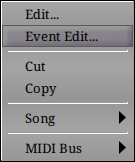
\includegraphics[scale=0.75]{pattern/pattern-right-click-menu.png}
   \caption{Existing Pattern, Right-Click Menu}
   \label{fig:pattern_window_right_click}
\end{figure}

   Here one can choose to edit the pattern, cut and copy the pattern,
   set the MIDI bus/channel, and more.
   One can also clear all performance data for the pattern.
   
   \begin{enumber}
      \item \textbf{Edit...}
      \item \textbf{Event Edit...}
      \item \textbf{Cut}
      \item \textbf{Copy}
      \item \textbf{Song/}
      \item \textbf{MIDI Bus/}
   \end{enumber}

   \setcounter{ItemCounter}{0}      % Reset the ItemCounter for this list.

   \itempar{Edit...}{pattern!edit}
   Edits an existing loop or pattern.
   Clicking this menu entry brings up the Pattern Editor
   so that one can modify the existing pattern.
   See \figureref{fig:pattern_edit_window}.
   Also known as the "sequence editor".

   \textbf{New:}
   In addition to right-clicking and selecting \textbf{Edit...}, the user
   \index{new!pattern ctrl-left-click}
   can Ctrl-left-click on the empty slot, or
   \index{new!empty slot double-click}
   double-click on the empty slot, to bring up the sequence
   editor.  For the double-click, the effect can be a bit confusing at first,
   because it currently also toggles the arming/mute status of the slot
   twice (leaving it as it was), as well.  For now, one must get used to it.

   \itempar{Event Edit...}{pattern!event edit}
   Edits an existing loop or pattern, but using a detailed event editor.
   Clicking this menu entry brings up the Event Editor
   so that one can view and modify the events in the existing pattern.
   See \figureref{fig:pattern_edit_window}.

   There are two things to note about this editor.
   First, this editor is not the same as the event editor pane in the pattern
   editor -- it shows all events at once, and shows them only in text format.
   Second, this editor is still a work in progress.
   See \sectionref{sec:seq64_event_editor} for more information.

   \itempar{Cut}{pattern!cut}
   Deletes and copies an existing loop or pattern.
   Note than one can also drag-and-drop a pattern into another cell.
   \textbf{Bug:}
   \index{bugs!pattern cut not dirty}
   Allow this operation works, it does not cause the user to be prompted if the
   application is exited.

   \itempar{Copy}{pattern!copy}
   Copies an existing loop or pattern.
   The pattern can then be pasted elsewhere in the Patterns panel.
   See \sectionref{subsubsec:seq64_patterns_pattern_slot}.

   \itempar{Song}{pattern!song}
   Clicking this menu entry brings up a small popup menu:

\begin{figure}[H]
   \centering 
   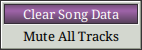
\includegraphics[scale=0.75]{pattern/pattern-menu-song.png}
   \caption{Existing Pattern, Right-Click Menu, Song}
   \label{fig:pattern_window_right_click_song}
\end{figure}

   \begin{enumber}
      \item \textbf{Clear Song Data}
      \item \textbf{Mute All Tracks}
   \end{enumber}

   \setcounter{ItemCounter}{0}      % Reset the ItemCounter for this list.

   \itempar{Clear Song Data}{pattern!clear song data}
   Selecting this filled-box right-click menu item causes that box's
   loop/pattern to be removed from the song.  This means
   that it disappears from the Song Editor window, and so will not
   be played when the song plays.

   \itempar{Mute All Tracks}{pattern!mute all tracks}
   Selecting this filled-box right-click menu item causes
   the tracks in the Song Editor to be muted.  Sometime it takes a few seconds
   for the user-interfaces to show this big change.

   \itempar{Midi Bus}{pattern!midi bus}
   Selecting this filled-box right-click menu item brings up a list
   of the 16 MIDI output busses that \textsl{Sequencer64} supports:

\begin{figure}[H]
   \centering 
   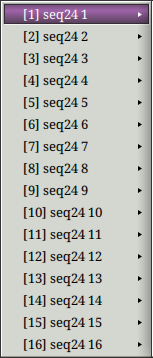
\includegraphics[scale=0.75]{pattern/pattern-menu-midi-bus.png}
   \caption{Existing Pattern, Right-Click Menu, MIDI Output Busses}
   \label{fig:pattern_window_right_click_midi_bus}
\end{figure}

   \textbf{New:}
   \index{new!--bus option}
   Note that another way of specifying the busses is to supply the
   new \texttt{--buss n} option.  This option is currently available
   only from the command line.  It causes \textsl{every} pattern in the MIDI
   file to be allocated to that buss number when loaded.  This option is
   meant for convenience or testing.  If you save the file, it will now
   have that buss number as part of each track's data.

   For each of these buss items, another pop-up menu allows one
   to specify the MIDI output channel for that buss:

\begin{figure}[H]
   \centering 
   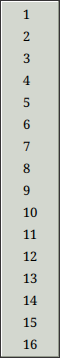
\includegraphics[scale=0.75]{pattern/pattern-menu-midi-bus-numbers.png}
   \caption{Existing Pattern, Right-Click Menu, MIDI Bus Ports}
   \label{fig:pattern_window_right_click_midi_bus_numbers}
\end{figure}

\subsubsection{Pattern Keys and Click}
\label{subsubsec:seq64_patterns_pattern_keys_and_clicks}

   This section recapitulates all the clicks and keys that perform actions
   in the Pattern windows.  Some additional clicks and keys are noted here
   as well.

\paragraph{Pattern Keys}
\label{paragraph:seq64_patterns_pattern_keys}

   Each pattern in the patterns panel can have a hot-key associated with it.
   \index{keys!hot-keys}

   \index{keys!pattern toggles}
   For each pattern, hitting its assigned keyboard key will
   also toggle its status between muted/unmuted (armed/unarmed).
   Below is the default grid that is
   mapped to the loops/patterns on the screen set.
   This grid can be changed in the Keyboard options tab, and is
   saved in the \textsl{keyboard-control} section of the
   \index{rc file}
   "rc" file.

   \begin{verbatim}
     [ 1   ][ 2   ][ 3   ][ 4   ][ 5   ][ 6   ][ 7   ][ 8   ]
     [ q   ][ w   ][ e   ][ r   ][ t   ][ y   ][ u   ][ i   ]
     [ a   ][ s   ][ d   ][ f   ][ g   ][ h   ][ j   ][ k   ]
     [ z   ][ x   ][ c   ][ v   ][ b   ][ n   ][ m   ][ ,   ]
   \end{verbatim}

   These characters are shown in the lower right corner of each
   pattern, as an aid to memory.

   These hot-keys can be modified

   \index{keys![}
   \index{keys!decrement set}
   The \texttt{[} and
   \index{keys!]}
   \index{keys!increment set}
   \texttt{]} keys on the keyboard
   switch between sets, either decrementing or incrementing the set number.

   The left and right Alt keys are, by default, set up in the
   \textbf{File / Options / Keyboard / Snapshot 1} and
   \textbf{Snapshot 2} fields to be used as "snapshot" keys.

   When one of these snapshot keys is pressed, the state of the patterns
   (which ones are armed versus unarmed) is instantly saved.  While the
   snapshot key is pressed, on can then change the state of the patterns to
   change how the song plays back.  When the snapshot key is released, the
   original saved state of the patterns is restored.

   \index{keys!alt}
   Holding \texttt{Alt} will save the state of playing patterns and restore
   them when \texttt{Alt} is lifted.

   The handling of \texttt{Alt} is generally taken over by the window
   manager, so there could be a need to change these items to some other
   keys.

%  \index{keys!left ctrl alt}
%  Holding \texttt{Left Ctrl} and \texttt{Alt} at the same time will enable
%  one to flip over to new patterns briefly and then flip right back upon
%  lifting \texttt{Alt}.  Not yet sure exactly what this means.

   \index{keys!right ctrl}
   \index{keys!queue}
   \index{queue!temporary}
	Holding \texttt{Right Ctrl} will queue a on/off toggle for a 
	sequence when the loop ends. This is the "queue" functionality.
   This means that the change in state of the pattern will not take hold
   immediately, but will kick in when the pattern restarts.

   This pending state is indicated by coloring the central box of the
   pattern grey, as shown in the following figure.

   Queue also works for mute/unmute patterns (groups). In this case every
   sequence will toggle its status after its individual loop end.

\begin{figure}[H]
   \centering 
   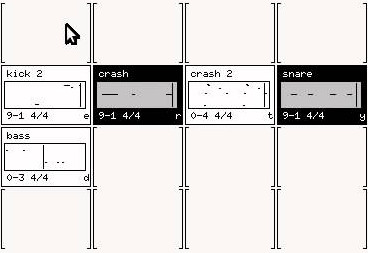
\includegraphics[scale=0.75]{pattern/seq24-queueing-coloration.jpg}
   \caption{Pattern Coloration when Queued}
   \label{fig:seq64_queueing_coloration}
\end{figure}

   Queue also works for mute/unmute 
	patterns (groups); in this case every sequence will toggle 
	its status after its individual loop end. 

   Of course, the Ctrl key is used to manage the GUI (e.g. Ctrl-q will
   unceremoniously quit the application), so one will usually want to change
   this key to something else in the
   \textbf{File / Options / Keyboard / Queue} field.
   The Super key (i.e. the Mod4 or Windows key) is a good candidate to
   replace the right Ctrl key, unless one has (like the author) configured
   the window manager to use the Super key modifier to manipulate windows
   and applications \textsl{(laughter ensues)}.

   \index{keys!replace}
   Note that there is also a "replace" key, which is the left Ctrl key by
   default.  Replacement is a form of muting/unmuting.  When the "replace"
   key is pressed while click a sequence, that sequence is unmuted, and all
   of the other sequences are muted.

   \index{keys!backslash}
   \index{keys!keep queue}
   \index{queue!permanent}
   \index{queue!keep queue}
	Pressing the "keep queue" key (by default, the backslash key)
   \index{rc file}
   assigned in the "rc" file.
	activates permanent queue mode until you use the temporary 
	queue function again pressing \texttt{Right Ctrl}. 

   This key can be changed in the
   \textbf{File / Options / Keyboard / Keep queue} field.

   There are more keys defined in the \textbf{Keyboard} dialog, and it is
   worth figuring out what they do, if not documented here.
   For a couple of short, but good, tutorials about using arming, queueing,
   and snapshots, see references \cite{wootangent1}
   and \cite{wootangent2}.

\paragraph{Pattern Clicks}
\label{paragraph:seq64_patterns_pattern_Clicks}

   \index{pattern!left click}
   \index{pattern!mute toggle}
   Left-clicking on a pattern-filled box will change its state
   \index{pattern!mute}
   \index{pattern!unmute}
   from muted (white background) to playing (black background) when
   the sequencer is running.

   \index{pattern!left ctrl left click}
   \index{keys!left ctrl}
   Holding down \texttt{Left Ctrl} while selecting a pattern
   with a left click will mute all other patterns and turn on the selected
   pattern.

   \index{pattern!left click-drag}
   By clicking and holding the left mouse button on a pattern,
   one can drag it to a new location on the grid.  The box
   will disappear while dragged, and reappear in the new location when
   dropped.  However, note that a pattern cannot be dragged if its
   Pattern Editor window is open.

   \index{pattern!right click}
   Right-clicking a pattern will bring up the appropriate context menus, as
   discussed earlier, depending on whether the pattern box is empty or
   filled.

   \index{pattern!middle click}
   Middle-click does nothing when the mouse rests inside a pattern box.

\subsection{Patterns / Bottom Panel}
\label{subsec:seq64_patterns_panel_bottom}

   The bottom panel of the Patterns window provides way to control the
   overall playback of the song.

\begin{figure}[H]
   \centering 
   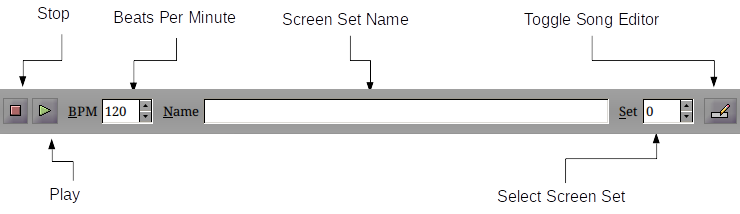
\includegraphics[scale=0.75]{pattern-window-bottom-panel-items.png}
   \caption{Patterns Panel, Bottom Panel Items}
   \label{fig:pattern_window_bottom_panel_items}
\end{figure}

   \begin{enumber}
      \item \textbf{Stop}
      \item \textbf{Play}
      \item \textbf{bpm}
      \item \textbf{Name}
      \item \textbf{Set}
      \item \textbf{Toggle Song Editor}
   \end{enumber}

   \setcounter{ItemCounter}{0}      % Reset the ItemCounter for this list.

   \itempar{Stop}{pattern!stop}
   The red squarebutton stops the playback of the song and all its patterns.
   It is not clear if it also sends MIDI Off messages on all notes.
   \index{keys!esc (stop)}
   The keystroke for stopping playback is the \texttt{Escape} character.
   It can be changed to \texttt{Space}, so that the space-bar then becomes a
   playback toggle key.

   \itempar{Play}{pattern!Play}
   The green triangular button starts the playback of the whole song.
   \index{keys!space (play)}
   The keystroke for starting playback is the \texttt{Space} character.

   \itempar{bpm}{pattern!bpm}
   The spin widget adjusts the "Beats Per Minute" or BPM value.  The
   range of this field is from 20 bpm to 500 bpm, with a default value of
   120 bpm.
   Although this field looks editable, it is not.  Most keystrokes
   that are entered actually toggle one of the pattern boxes.
   However, the following keys can also modify the BPM in small increments:
   \index{keys!semicolon} The \texttt{semicolon} reduces the BPM;
   \index{keys!apostrophe} The \texttt{apostrophe} increases the BPM.

   \itempar{Name}{pattern!set name}
   Each of the 32 available screen sets can be given a name by entering it
   into this field.

   \textbf{Bug:}
   \index{bugs!set name has side-effect}
   While one is typing in the name of the set in this field, the keystrokes
   will affect the panel window, causing playback to start and pattern
   boxes to be toggled!

   \itempar{Set}{pattern!set number}
   This spin widget selects the current screen set.  The values in this
   field range from 0 to 31, and default to 0.
   Although this field looks editable, it is not.

   \textbf{Bug:}
   \index{bugs!set number has side-effect}
   While one is typing in the number of the set in this field, the keystrokes
   will affect the panel window as well.

   \itempar{Toggle Song Editor}{pattern!toggle song editor}
   Pressing this button toggles the presence on-screen of the Song
   Editor.

%-------------------------------------------------------------------------------
% vim: ts=3 sw=3 et ft=tex
%-------------------------------------------------------------------------------


% Pattern Editor

%-------------------------------------------------------------------------------
% seq64_pattern_editor
%-------------------------------------------------------------------------------
%
% \file        seq64_pattern_editor.tex
% \library     Documents
% \author      Chris Ahlstrom
% \date        2015-08-31
% \update      2016-09-06
% \version     $Revision$
% \license     $XPC_GPL_LICENSE$
%
%-------------------------------------------------------------------------------

\section{Pattern Editor}
\label{sec:seq64_pattern_editor}

   The \textsl{Sequencer64 Pattern Editor} is used to edit and preview a
   pattern, as well as to configure its buss and channel settings.
   In programmer's jargon, this window is represented by the seqroll class (and
   the other "seq" classes).

\begin{figure}[H]
   \centering 
%  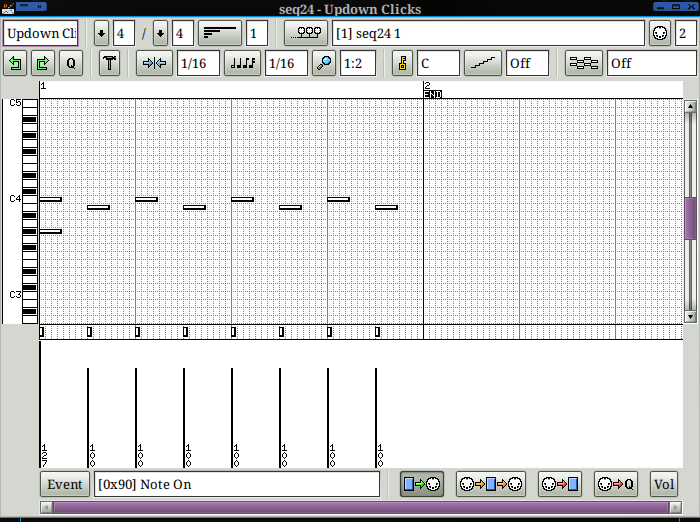
\includegraphics[scale=0.75]{pattern/pattern-edit-window.png}
%  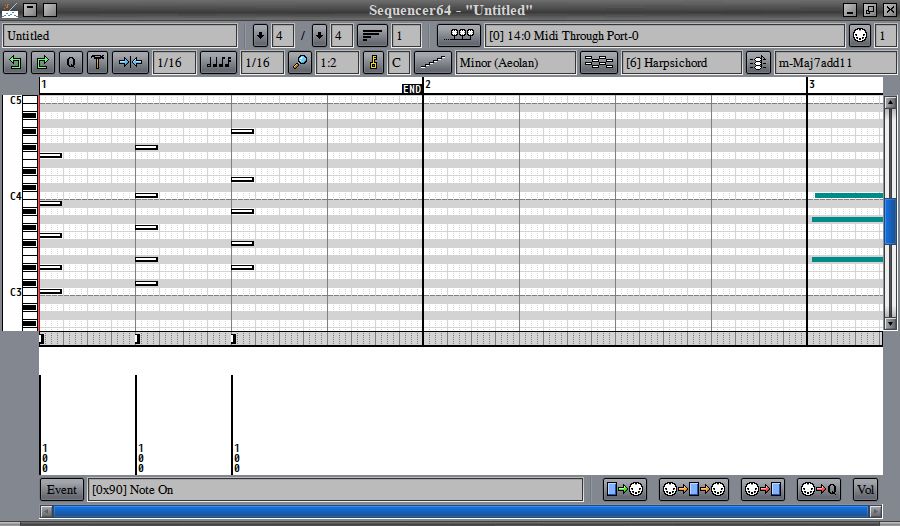
\includegraphics[scale=0.75]{new/pattern_editor_chords-0_9_14.png}
   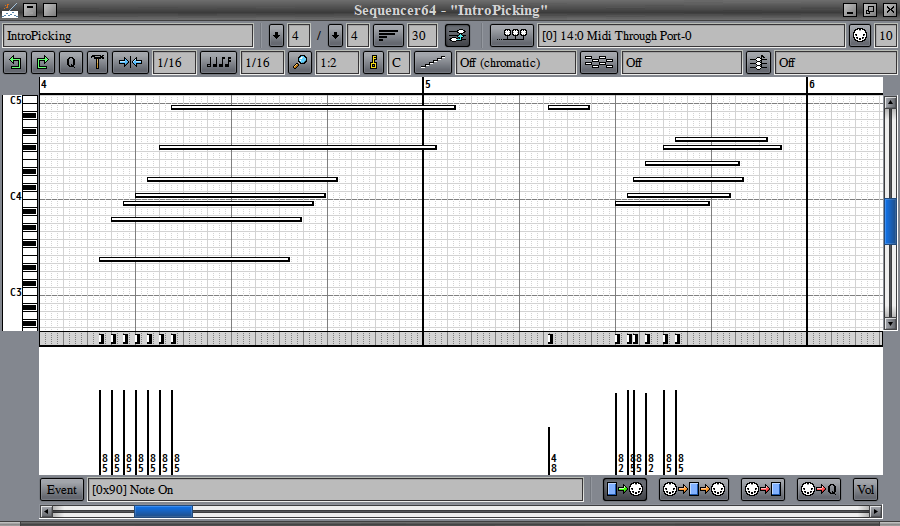
\includegraphics[scale=0.75]{new/pattern_editor_transpose-0_9_15.png}
   \caption{Pattern Edit Window}
   \label{fig:pattern_edit_window}
\end{figure}

   This dialog is complex.
   For exposition, we break it into some common actions, a first panel, a
   second panel, a bottom panel, and a piano-roll/events section.

   \begin{enumber}
      \item \textbf{First Panel}
      \item \textbf{Second Panel}
      \item \textbf{Piano-Roll/Events Panel}
      \item \textbf{Bottom Panel}
      \item \textbf{Common Actions}
   \end{enumber}

   Before we describe this window, there are some peculiarities to recognize.
   First, if the pattern is empty when play is started, the progress bar will
   not move.  It moves only if there are events to play in the pattern.
   Second, to add a note, one must press the right mouse button (the pointer
   changes to a pencil) and, while holding it, press the left mouse button.  Or
   click in the pattern editor, press
   \index{keys!p}
   "p" to select the "pencil" or "paint" mode, then
   \index{mouse!left-click-drag}
   left-click-drag to add notes.
   \index{keys!x}
   Press "x" to "eXit" or "eXscape" from that mode.  Also remember
   that notes are drawn only with the length selected by the "notes" button
   near the top of the pattern window.  There are some other tricks to
   modifying the new notes that are described later.

   Also new with \textsl{Sequencer64}, and not in \textsl{Seq24}, is the
   automatic horizontal scrolling of the sequence/pattern editor window when
   playback moves the progress bar outside of the current frame of data.  This
   feature makes it easier to follow patterns that are longer than a measure or
   two.
   
   Note that \textsl{Sequencer64} also provides a way to restart the progress
   bar within the pattern without resetting it to the beginning of the pattern.
   \index{pause} This new feature is called "pause".  It can be accessed by the
   \index{keys!.}
   \index{keys!pause}
   new pause key (which defaults to the period character) or by the pause
   button, which appears when playback is underway.  (Note that this feature
   can be disabled if the application is built via source code.)

\subsection{Pattern Editor / First Panel}
\label{subsec:seq64_pattern_editor_first}

   The top bar (horizontal panel) of the Pattern (sequence) Editor
   lets one change the name of
   the pattern, the time signature of the piece, how long the loop is, and
   some other configuration items.

\begin{figure}[H]
   \centering 
   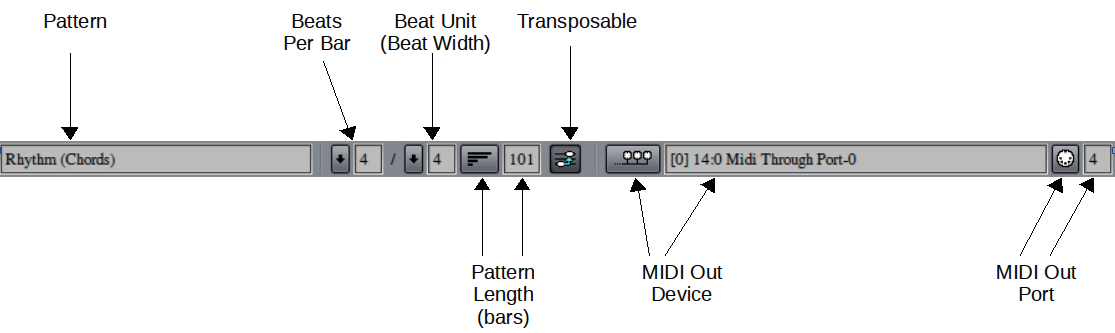
\includegraphics[scale=0.55]{pattern/pattern-edit-first-panel-items.png}
   \caption{Pattern Editor, First Panel Items}
   \label{fig:pattern_editor_first_panel_items}
\end{figure}

   In recent versions of \textsl{Sequencer64}, a "sequence-is-transposable"
   feature has been added, as shown above.

% \begin{figure}[H]
%    \centering 
%    
\includegraphics[scale=0.75]{new/pattern_editor_top_panel-0_9_15.png}
%    \caption{Pattern Editor, First Panel Emphasizing Transposable Button}
%    \label{fig:pattern_editor_first_panel_transposable}
% \end{figure}

   \begin{enumber}
      \item \textbf{Pattern Name}
      \item \textbf{Beats Per Bar}
      \item \textbf{Beat Unit (Beat Width)}
      \item \textbf{Pattern Length}
      \item \textbf{Transposable (toggle)}
      \item \textbf{MIDI Out Device}
      \item \textbf{MIDI Out Port}
   \end{enumber}

   \setcounter{ItemCounter}{0}      % Reset the ItemCounter for this list.

   \itempar{Pattern Name}{pattern editor!name}
   Provides the name of the pattern.
   This name should be short and memorable.
   It is displayed in the Patterns window, on the top line of its pattern
   box/slot.

   \itempar{Beats Per Bar}{pattern editor!beats/bar}
   Part of the time signature, and specifies the number of beat units per bar.
   The possible values range from 1 to 16.

   \itempar{Beat Unit (Beat Width)}{pattern editor!beat unit}
   \index{pattern editors!beat width}
   \index{beat width}
   Part of the time signature, and specifies the size of the beat unit:
   1 for whole notes; 2 for half notes; 4 for quarter notes; 8 for eight notes;
   and 16 for sixteenth notes.
   The whole time signature is display at the bottom center of a pattern
   box/slot.

   \itempar{Pattern Length}{pattern editor!length}
   Sets the length of the current pattern, in measures.
   The possible values range from 1 to 16, then 32, and 64.
   \textsl{However}, when opening or importing a non-\textsl{Sequencer64}
   MIDI tune the length of each track will be use, and so other values
   are possible; they just cannot be set via the user-interface.

   Note that bringing up a short sequence (one less than one measure or bar in
   length) in the pattern editor will adjust the sequence to pad it to the
   length of one measure.  For example, a sequence containing just one program
   change will be padded to the size of a full measure.
   This adjustment makes it show progress more smoothly in the main window when
   the sequence is playing.
   \index{pattern editor!progress bar}
   \textsl{Sequencer64} will, when it reads such a short sequence
   from a MIDI file (whether foreign or native to \textsl{Sequencer64}),
   pre-pad it to the length of a measure, so that it will always show smooth
   progress.

   \textsl{(It would sure be nice to have a value that represents
   "indefinite", so that the loop or pattern would be more like a track,
   and not be repeatable.  Or perhaps add lengths of 128 and 200.  The length
   of the longest track in our sample is 101 measures.
   Also nice would be a "one-shot"
   pattern, useful for live intro patterns, for example.)}

   \itempar{Transpose Toggle}{pattern editor!transpose toggle}
   This item if enabled, allows the sequence to be transposed by the global
   transpose selection made in the song editor.  If enabled, the button will be
   highlighted as per the current desktop theme.  Patterns for drums should,
   in general, not be transposable.

   \itempar{MIDI Out Device (Buss)}{pattern editor!midi out device}
   This setting specifies one of the 16 MIDI output busses provided by
   \textsl{Sequencer64}.  The settings look a lot like
   \figureref{fig:pattern_window_right_click_midi_bus}.

   \itempar{MIDI Out Port (Channel)}{pattern editor!midi out port}
   This settings select the MIDI output channel, or port.
   The possible values range from 1 to 16.
   If instruments are defined in the "user" configuration file
   to that device and channel, they will be shown.

\subsection{Pattern Editor / Second Panel}
\label{subsec:seq64_pattern_editor_second}

   The second horizontal panel of the Pattern Editor provides a number
   of additional settings.

\begin{figure}[H]
   \centering 
   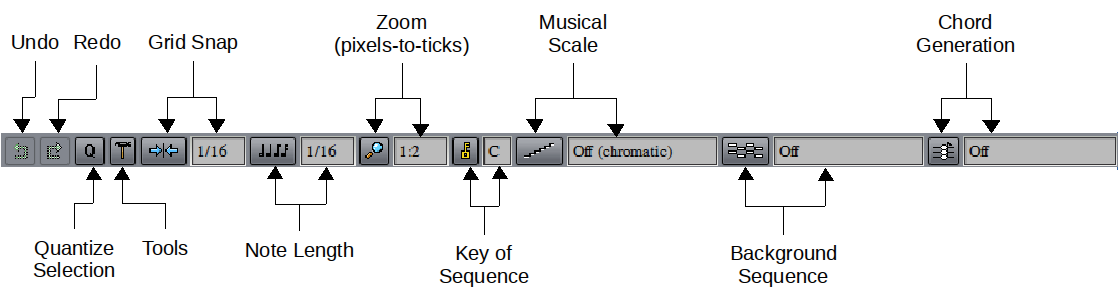
\includegraphics[scale=0.55]{pattern/pattern-edit-second-panel-items.png}
   \caption{Pattern Editor, Second Panel Items}
   \label{fig:pattern_editor_main_panel_items}
\end{figure}

   If \textsl{Sequencer64} is built with the new chord-generation option
   built in (the default), then the second panel is wider to make room for an
   addition user-interface item, shown at the right of the figure above.

% \begin{figure}[H]
%    \centering 
%    
\includegraphics[scale=0.75]{new/pattern_editor_second_panel-0_9_14.png}
%    \caption{Pattern Editor, Second Panel Items Emphasizing Chord Button}
%    \label{fig:pattern_editor_main_panel_chord_button}
% \end{figure}

   \begin{enumber}
      \item \textbf{Undo}
      \item \textbf{Redo}
      \item \textbf{Quantize Selection}
      \item \textbf{Tools}
      \item \textbf{Grid Snap}
      \item \textbf{Note Length}
      \item \textbf{Zoom}
      \item \textbf{Key of Sequence}
      \item \textbf{Musical Scale}
      \item \textbf{Background Sequence}
      \item \textbf{Chord Generation}
   \end{enumber}

   \setcounter{ItemCounter}{0}      % Reset the ItemCounter for this list.

   \itempar{Undo}{pattern editor!undo}
   The Undo button will roll back any changes to the pattern from this
   session.
   It will roll back one change each time it is pressed.
   It is not certain what the undo limit (if any) is, however.
   \index{keys!ctrl-z}
   Pressing \texttt{Ctrl-Z} is the same as using the \textbf{Undo} button.

   \itempar{Redo}{pattern editor!redo}
   The Redo button will restore any undone changes to the pattern from this
   session.
   It will restore one change each time it is pressed.
   It is not certain what the redo limit is, however.
   There doesn't seem to be a "Redo" key in the pattern editor.

   \itempar{Quantize Selection}{pattern editor!quantize}
   Pressing this button will quantize the selected events, presumably as per
   the \textbf{Grid Snap} setting.

   \itempar{Tools}{pattern editor!tools}
   This button brings up a nested menu of tools for modifying selected
   events and notes.

\begin{figure}[H]
   \centering 
   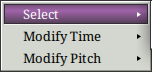
\includegraphics[scale=0.75]{pattern/tools-first-menu.png}
   \caption{Tools, Context Menu}
   \label{fig:pattern_editor_tools_first_menu}
\end{figure}

   \begin{enumber}
      \item \textbf{Select}
      \item \textbf{Modify Time}
      \item \textbf{Modify Pitch}
   \end{enumber}

   $\bullet$ \textbf{Select} provides two sets of selections for notes:
   \begin{itemize}
      \item \textbf{All Notes}, which selects all notes in the pattern;
         Note that \index{keys!ctrl-a} \texttt{Ctrl-A} will also select
         all of the events in the pattern editor.
      \item \textbf{Inverse Notes}, which inverts the selection of notes.
   \end{itemize}

   Other event-selection actions are provided:

   \begin{itemize}
      \item \index{mouse!left-click}
         \textbf{Left Click}.
         Pressing the left button on a note or a event deselects all other
         notes or events, and selects the item clicked on.
      \item \index{mouse!ctrl-left-click}
         \textbf{Ctrl Left Click}.
         Pressing the \texttt{Ctrl} key and the left button on a note or an
         unselected event \textsl{adds} that event to the selection.
         This is a bit different from conventional selection addition
         in other applications, which tend to use the \texttt{Shift} key.
      \item \index{mouse!left-click-drag}
         \textbf{Left Click Drag}.
         Pressing the left mouse button and dragging also lets one
         select multiple events and notes.
      \item \index{mouse!ctrl-left-click-drag}
         \textbf{Ctrl Left Click Drag}.
         \begin{itemize}
            \item Pressing the \texttt{Ctrl} while left-click-dragging
               \textsl{on unselected events} lets one make additional
               selections of multiple events and notes.
            \item Pressing the \texttt{Ctrl} while left-click-dragging
               \textsl{on an already-selected event} lets one stretch or
               compress the lengths of multiple notes in the selection.
         \end{itemize}
   \end{itemize}

   There are many things that can be done with selected notes, as will be seen
   in the following paragraphs.

   \index{modify event-data}
   $\bullet$ \textbf{Modify Event Data} offers a way to change the event data
   (the lower pane of the pattern editor).
   By left-dragging the mouse in the data pane across the value lines that are
   shown, the values are chopped or set to the height of the mouse pointer at
   each event.
   When notes are selected, and the
   mouse is used to change the values (heights) of the lines in the event-data
   area,
   \textsl{only the events that are selected} are changed.  The data-values of
   selected events are left unchanged.  A cool feature from \textsl{Seq24}.

   \index{modify time}
   $\bullet$ \textbf{Modify Time} offers two ways to tweak the timing of the
   selected note:
   \index{quantize}
   \textbf{Quantize Selected Notes}, which quantizes the selected
   notes, presumably the same way as the \textbf{Quantize} ("\textbf{Q}")
   button;
   \index{tighten}
   \textbf{Tighten Selected Notes}, which presumably is a less
   strict form of quantization.
   \textbf{TODO:}
   \index{"todo!what is tighten"}
   Need more information about the meaning of "tightening a note".

   \index{modify pitch}
   $\bullet$ \textbf{Modify Pitch} has only one entry by default,
   \textbf{Transpose Selected} (not shown).
   Selecting the \textbf{Transpose Selected} entry
   brings up the following sub-menu:

\begin{figure}[H]
   \centering 
   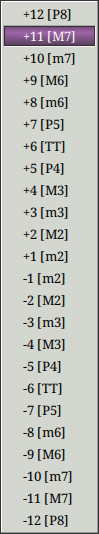
\includegraphics[scale=0.75]{pattern/tools-transpose-selected-menu.png}
   \caption{Tools, Transpose Selected Values}
   \label{fig:pattern_editor_tools_transpose_selected_menu}
\end{figure}

   $\bullet$ If the user has selected a
   \textbf{Musical Scale} setting other than \textbf{Off},
   then \textbf{Modify Pitch} has two entries:
   \textbf{Transpose Selected}, discussed above, plus
   another sub-menu,
   \textbf{Harmonic Transpose Selected}, which makes sure that all
   transpositions stay on the selected scale.

   Note that one can also modify the pitch of selected notes by the
   \index{mouse!left-click-drag}
   left-click-drag action, or by moving the selection using the
   \index{keys!down-arrow}
   \index{keys!up-arrow}
   up-arrow or down-arrow keys.

\begin{figure}[H]
   \centering 
   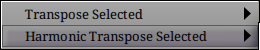
\includegraphics[scale=0.75]{pattern/tools-transpose-and-harmonic-selected-menu.png}
   \caption{Tools, Two "Transpose" Menus}
   \label{fig:pattern_editor_tools_two_transpose_menus}
\end{figure}

   Remember that only the \textbf{Transpose Selected} entry is shown if the
   \textbf{Musical Scale} setting is \textbf{Off}.

   Selecting the \textbf{Harmonic Transpose Selected} entry brings up the
   following sub-menu:

\begin{figure}[H]
   \centering 
   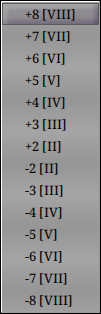
\includegraphics[scale=0.75]{pattern/tools-harmonic-transpose-selected-menu.png}
   \caption{Tools, Harmonic Transpose Selected Values}
   \label{fig:pattern_editor_tools_harmonic_transpose_menu}
\end{figure}

   Again, the harmonic-transpose option will not be available unless a scale
   has been selected.

   \itempar{Grid Snap}{pattern editor!grid snap}
   Grid snap selects where the notes will be drawn.
   The following values are supported:
   1, 1/2, 1/4, 1/8, 1/16, 1/32, 1/64, and 1/128.
   Additional values are also supported:
   1/3, 1/6, 1/12/, 1/24, 1/48, 1/96, and 1/192.

   \itempar{Note Length}{pattern editor!note length}
   Note Length determines the duration of the inserted notes.
   Like the \textbf{Grid Snap} values,
   the following values are supported:
   1, 1/2, 1/4, 1/8, 1/16, 1/32, 1/64, and 1/128.
   Additional values are also supported:
   1/3, 1/6, 1/12/, 1/24, 1/48, 1/96, and 1/192.

   \itempar{Zoom}{pattern editor!zoom}
   Zoom is the relation between MIDI pixels and ticks, written as
   "pixels:ticks", where "ticks" is really the "pulses" in "PPQN".
   For example, 1:4 = 4 ticks per pixel.
   Supported values are 1:1, 1:2, 1:4, 1:8, 1:16, and 1:32, along with
   more new values to support higher PPQN tunes: 1:64, 1:128, 1:256, and
   1:512.
   The default zoom is 2 for the standard PPQN value, 192, but it
   increases for higher PPQN values.
   This is the zoom of the Pattern Editor.  As the right number goes higher,
   the effect is to zoom out, and show more of the pattern at once.
   In fact, it is probably better to list them as ticks (pulses) per pixel:

   \begin{itemize}
      \item 1 pulse per pixel
      \item 2 pulses per pixel (default value)
      \item 4 pulses per pixel
      \item 8 pulses per pixel
      \item 16 pulses per pixel
      \item 32 pulses per pixel (same as Song Editor)
      \item . . .
      \item 512 pulses per pixel
   \end{itemize}

   \textbf{New:}
   \index{new!zoom keys}
   \index{keys!0}
   \index{keys!z}
   \index{keys!shift-z}
   After one has left-clicked in the piano roll, the "z", "Z", and "0"
   can be used to zoom the piano-roll view.  The "z" key zooms out, the "Z" key
   zooms in, and the "0" key resets the zoom to the default value.
   The zoom feature also modifies the time-line (measures indicator) and
   the data area.
   If, for some reason, the data area and piano-roll get out of sync, click on
   the horizontal scroll bar to force the views to redraw properly.

   \index{song editor!zoom}
   Note that the Song Editor, which now has zoom functionality (through
   the "z", "Z", and "0" keystrokes only),
   has a default resolution of 32 pulses per pixel, so, by default, it has
   16 times the resolution of the Pattern Editor.

   \itempar{Key of Sequence}{pattern editor!key}
   Selects the desired key for the pattern.  The following scales are
   supported:  C, C\#, D, D\#, E, F, F\#, G, G\#, A, A\#, and B.
   Note that changing the \textbf{Key} will also shift the marked notes
   for the \textbf{Musical Scale} setting.

   \textbf{New:}
   \index{new!save musical key}
   As of version 0.9.9.8, the key that a sequence is set to is
   now saved in the MIDI file along with the rest of the data for the sequence.
   \textbf{However},
   it turns out that a change made to the key, scale, or background sequence in
   the sequence editor is saved in that editor, so that opening another sequence
   will apply the same settings to that sequence.  This is a feature, now
   more rigorously supported, as noted below.

   If the global-sequence-feature is enabled, and the user selects
   a different key, scale, or background sequence in the sequence editor, 
   then all sequences will share the selected key, scale, or background
   sequence.  Furthermore, these settings are saved in the "proprietary"
   section of the MIDI file, where they are available for all sequences.

   If the global-sequence-feature is not enabled, and the user selects
   a different key, scale, or background sequence in the sequence editor, 
   then only that sequence will use the selected key, scale, or background.
   The key, scale, or background sequence change will be saved in the MIDI file
   only for that sequence, as a SeqSpec meta event.

   The global-sequence-feature setting can be made in the "user" configuration
   file.

   \itempar{Musical Scale}{pattern editor!scale}
   Selects the desired scale for the pattern.
   When a scale is selected, the following features are supported:

   \begin{itemize}
      \item The notes that are not in the scale are shown as grey in the piano
         roll, to make it easier to key all notes in-scale.
      \item When harmonic transposition is performed, the notes are shifted
         so that they remain in scale.
      \item The exact notes that are considered "in-scale" depend also on the 
         exact value of the \textbf{Key of Sequence} setting.
   \end{itemize}

   \textbf{New:}
   \index{new!musical scales}
   Originally, only the following scales were supported: Off, Major, and Minor.
   Now, the following scales are supported:

   \begin{itemize}
      \item \textbf{Off (chromatic)}
      \item \textbf{Major}
      \item \textbf{Minor}
      \item \textbf{Harmonic Minor}
      \item \textbf{Melodic Minor}
      \item \textbf{Whole Tone}
      \item \textbf{Blues}
      \item \textbf{Major Pentatonic}
      \item \textbf{Minor Pentatonic}
   \end{itemize}

   Please let us know of any mistakes found in the new scales.
   Also please note that the \textbf{Melodic Minor} scale is supposed to
   descend in the same was as the natural \textbf{Minor} scale, but
   currently there is no way to support that trick in
   \textsl{Sequencer64}.

\begin{figure}[H]
   \centering 
%  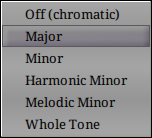
\includegraphics[scale=0.75]{pattern/scales-menu.png}
   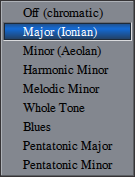
\includegraphics[scale=1.0]{new/scales-menu.png}
   \caption{Scales Currently Supported in Sequencer64}
   \label{fig:pattern_editor_available_scales}
\end{figure}

   One can select which \textbf{Musical Scale} and
   \textbf{Key} the piece is in,
   and \textsl{Sequencer64} will grey those keys on the piano-roll that
   are \textsl{not} in the selected scale for the selected key.
   This is purely a visual thing; a user can still add off-key notes.
   This effect is shown for the C Major scale in the following figure:

\begin{figure}[H]
   \centering 
   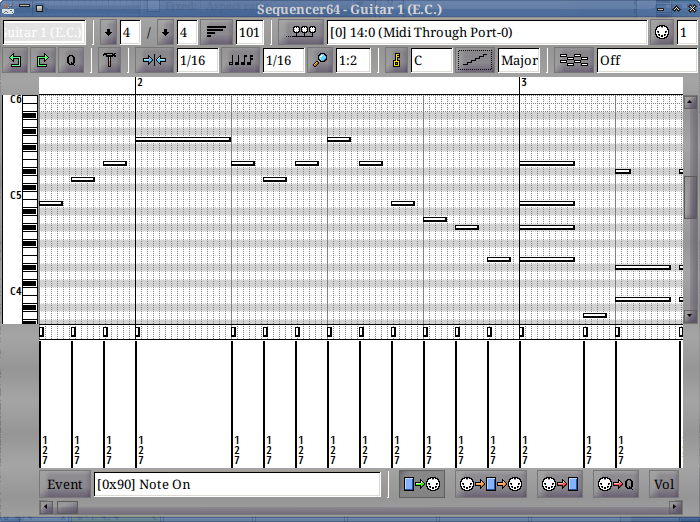
\includegraphics[scale=0.75]{pattern/major-scale-masking.png}
   \caption{C Major Scale Masking}
   \label{fig:pattern_editor_major_scale_masking}
\end{figure}

   This feature makes it a bit easier to stay in key while playing and
   recording.  Note that the scale will shift when a different
   \textbf{Key} is selected.

   \textbf{New:}
   \index{new!save musical scale}
   The scale that a sequence is set to is
   now saved in the MIDI file along with the rest of the data for the sequence.
   \textbf{However},
   it turns out that a change made to the key, scale, or background sequence in
   the sequence editor is saved in the editor, so that opening another sequence
   will apply the same settings to that sequence.  This is a feature.
   The feature had some quirks, which are fixed, and it is now
   an optional feature.
   Also, the user has the option of applying the key/scale/background-sequence
   either globally (all sequences) or locally, per-sequence, with each sequence
   holding its key, scale, and background-sequence settings in
   SeqSpec meta events.

   \itempar{Background Sequence}{pattern editor!background sequence}
   One can select another pattern to draw on the background to help with
   writing corresponding parts.
   The button brings up a small menu with values of \textbf{Off} and
   \textbf{[0]}.  The 0 is a set number. Sets are numbered from 0 to 31.
   Additional set numbers appear in the menu for each set that has data in it.
   Under the \textbf{0}
   entry, a menu like the following appears:

\begin{figure}[H]
   \centering 
   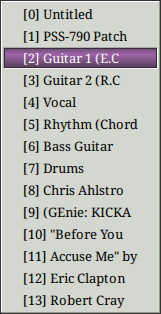
\includegraphics[scale=0.75]{pattern/background-sequence-menu.png}
   \caption{Sample Background Sequence Values}
   \label{fig:pattern_editor_background_sequence_menu}
\end{figure}

   Once the desired pattern is selected from that list, it appears as
   dark cyan note bars, along with the notes that are part of the pattern.
   (Also note the orange selected notes and events in the following figure.)

\begin{figure}[H]
   \centering 
   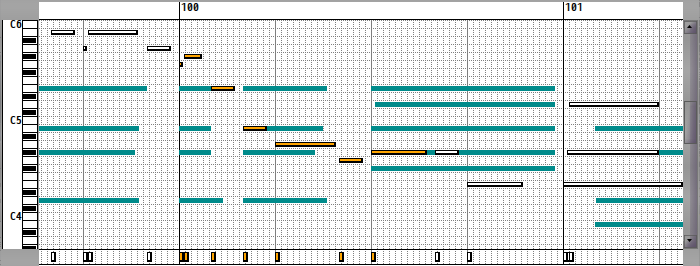
\includegraphics[scale=0.75]{pattern/background-sequence-notes.png}
   \caption{Background Sequence Notes}
   \label{fig:pattern_editor_background_sequence_notes}
\end{figure}

   The dark cyan notes shown represent a rhythm pattern.

   \textbf{New:}
   \index{new!save background seqeuence}
   The background sequence that a sequence shows is now saved in the MIDI file
   along with the rest of the data for the sequence.
   \textbf{However},
   it turns out that a change made to the key, scale, or background sequence in
   the sequence editor is saved in the editor, so that opening another sequence
   will apply the same settings to that sequence.  This is a feature, now
   more rigorously supported, as noted earlier.

   \itempar{Chord Generation}{pattern editor!chord generation}
   As of version 0.9.9.14, the ability to insert chords with one
   click has been added.  This feature comes from user "stazed"
   and his \textsl{Seq32} project (\cite{seq32}).

\begin{figure}[H]
   \centering 
   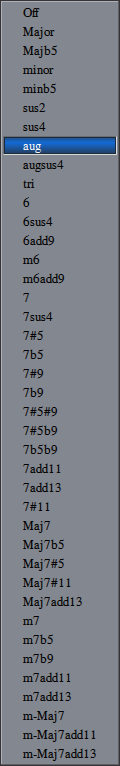
\includegraphics[scale=1.0]{new/chords_menu-0_9_14.png}
   \caption{Chord Generation Menu}
   \label{fig:pattern_editor_chords_menu}
\end{figure}

   The figure shows the menu broken into two pieces.
   Once a value other than \textbf{Off} is selected, a left-click
   in drawing mode will add multiple notes representing the chord
   created, with the clicked note value as the base of the chord.

\subsection{Pattern Editor / Piano Roll}
\label{subsec:seq64_pattern_editor_piano_roll}

   The piano roll is the center of the pattern editor.  It is accompanied by a
   \index{event area}
   thin "event bar" (or "event area", or "event strip") just below it,
   \index{data area}
   and a taller "data bar" or "data area" just below that.

   The piano roll is the heart of the pattern (loop, sequence) editor.
   While it is very similar to note editors in other sequencers, it is a bit
   different in feel.  A good mouse with 3 or more buttons is practically a
   necessity for editing, though we have made it more
   usable with some pretty crummy trackpads now common on modern laptops,
   and with keystrokes.
   We tend to like the Logitech Marble Mouse, an
   ambidextrous USB trackball.  It has four buttons, and we use the
   \texttt{contrib/scripts/marblemouse} script to set up the left small
   button as a middle button.  The script merely makes the following call:

   \begin{verbatim}
      xmodmap -e "pointer = 1 8 3 4 9 6 7 2 5 10 11"
   \end{verbatim}

   Editing is much easier after making that setting.   Of course, keystrokes
   and additional mouse configuration have been added to make editing easier
   even without a good mouse.
   For example, one can page up and down vertically in the piano roll using the
   \index{keys!page-up} Page Up and 
   \index{keys!page-down} Page Down keys.
   One can go to the top using the 
   \index{keys!home} Home key, and
   to the bottom using the
   \index{keys!end} End key.
   One can page left and right horizontally in the piano roll using the
   \index{keys!shift-page-up} Shift Page Up and 
   \index{keys!shift-page-down} Shift Page Down keys.
   One can go to the leftmost position using the 
   \index{keys!shift-home} Home key,
   and to the rightmost position using the
   \index{keys!shift-end} End key,

\subsubsection{Pattern Editor / Piano Roll Items}
\label{subsubsec:seq64_pattern_editor_piano_roll_items}

\begin{figure}[H]
   \centering 
   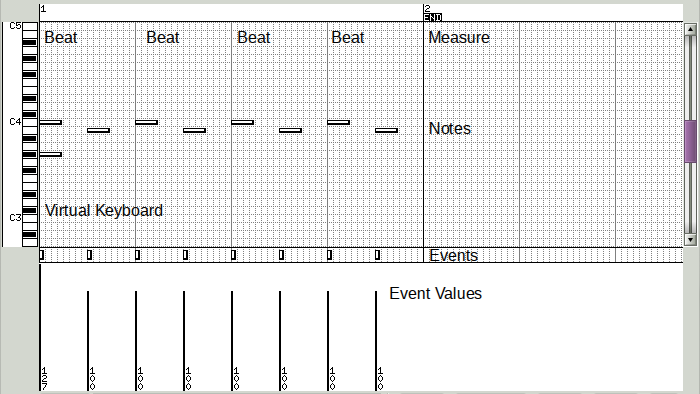
\includegraphics[scale=0.75]{pattern/pattern-edit-piano-roll-items.png}
   \caption{Pattern Editor, Piano Roll Items}
   \label{fig:pattern_editor_piano_roll_items}
\end{figure}

   \begin{enumber}
      \item \textbf{Beat}
      \item \textbf{Measure}
      \item \textbf{Virtual Keyboard}
      \item \textbf{Notes}
      \item \textbf{Events}
      \item \textbf{Event Values}
   \end{enumber}

   \setcounter{ItemCounter}{0}      % Reset the ItemCounter for this list.

   \itempar{Beat}{piano roll!beat}
   The light vertical lines represent the beats defined by the configuration
   for the pattern.

   \itempar{Measure}{piano roll!measure}
   The heavy vertical lines represent the measures defined by the
   configuration for the pattern.
   \index{pattern!end marker}
   Also note that the end of the pattern
   occurs at a measure, and is marked by a blocky \textbf{END} marker.

   \itempar{Virtual Keyboard}{piano roll!virtual keyboard}
   The virtual keyboard is a fairly powerful interface.  It shows,
   by shadowing, which note on the keyboard one will be drawing. It can be
   played with a mouse, using left-clicks, to preview a short motif.
   It can show marks to indicate off-scale notes, to make them easy to
   avoid.  Every octave, a note letter and octave number are shown, as in
   "C4".  If there is a difference scale in force, then the letter changes to
   match, as in "F\#5".

   \index{virtual keyboard!right-click}
   A right-click anywhere in the virtual keyboard area toggles the display
   between the octave note letters and the MIDI note numbers (only every other
   one is displayed due to space, to avoid cramped numbering).
   The following figure shows both views, superimposed for comparison.

\begin{figure}[H]
   \centering 
   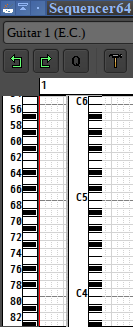
\includegraphics[scale=0.75]{pattern/pattern-edit-window-key-numbers.png}
   \caption{Pattern Editor, Virtual Keyboard Number and Note Views}
   \label{fig:pattern_editor_key_numbers}
\end{figure}

   \itempar{Notes}{piano roll!notes}
   Musical notes are indicated by thick horizontal bars with white
   centers.  Each bar provides
   a visual representation of the pitch of a note and the length of a note.

   \itempar{Events}{piano roll!events}
   \index{events strip}
   The small (just a few pixels high) events strip shows discrete events,
   such as Note On and Note Off and their velocities, or various Controller
   items and their values.  We recommend not trying to edit or select events
   in that pane, in general, but it is a good way to add events.
   Either
   \index{mouse!left-click}
   left-click (to add one event),
   \index{mouse!left-click-drag}
   or left-click-drag horizontally (to add a
   series of events at the current note resolution.)  One can also
   left-click in that section,
   \index{keys!p}
   then hit the "p" key to go into "paint" mode,
   \index{keys!x}
   and hit the "x" key to escape that mode.

   \itempar{Event Values}{piano roll!event values}
   The events values for the currently selected category of events are shown
   in this window as vertical lines of a height proportional to the value.
   These values can be easily modified by
   \index{mouse!left-click-drag}
   left-click-dragging the
   mouse past each line, to chop it off at the given value.  Easier to try
   it than explain it.
   \index{mouse!right-click-drag}
   Right-click-drag also works the same.

\subsubsection{Pattern Editor / Event Editing}
\label{subsubsec:seq64_pattern_editor_event_editing}

   \index{draw mode}
   \index{paint mode}
   When we say "editing" in the context of the piano roll, in part we mean that
   we will "draw" or "paint" notes.
   Drawing, modifying, copying, and deleting
   notes is actually very elegant in \textsl{Seqeuencer64} (and in
   \textsl{Seq24}).

   Note editing is a bit different with \textsl{Sequencer64}, since it
   requires two mouse buttons in many cases.  There are some new
   laptop touchpads that really have only one mouse button, and
   use positioning to determine if the click is a left-click or a right-click.
   Two-fingered actions are devoted to scrolling, so that there is no way
   to generate a Linux middle-click.
   One solution is to use a four-button USB trackball
   configued with an easy middle-button setup.
   It's easier than a touchpad, anyway.
   So we've coded up a couple of solutions to this middle-click problem.

   Note that, if only a middle-button is needed, ctrl-left-button will simulate
   that button.  Also note the "Mod4 mode" for the right-click action, and the
   "p" and "x" keys for getting in and out of "paint mode", discussed
   elsewhere.

   \index{new!mod4 mode}
   \index{keys!mod4}
   \index{pattern editor!mod4}
   \textbf{New:}
   There is a feature to allow the Mod4 (the Super or Windows) key to keep the
   right-click in force even after it is released.  See \ref{new_mod4_mode}.
   Basically, pressing Mod4 before releasing the right-click that allows
   note-adding, keeps note-adding in force after the right-click is released.
   Now notes can be added at will with the left mouse button.  Right-click
   again to leave the note-adding mode.

   \textbf{New:}
   \index{new!paint mode}
   Another way to turn on the paint mode has been added.
   To turn on the paint mode, first make sure that the piano roll has the
   keyboard focus by left-clicking in it, then press the
   \index{keys!p}
   \texttt{p} key while in the sequence editor.
   This is just like pressing the right mouse button, but the draw/paint mode
   sticks (as if the Mod4 mode were in force).
   To get out of the paint mode, press the
   \index{keys!x}
   \texttt{x} key while in the sequence editor, to "x-scape" (get it? get it?)
   from the paint mode.
   These keys also work while the sequence is playing.

   The \texttt{p} and \texttt{x} keys also works in the small event strip just
   above the white data area.  The Mod4-right-click feature does not
   yet work in that aread of the user interface, but the \texttt{p} key does.

\paragraph{Editing Note Events}
\label{paragraph:seq64_pattern_editor_note_events}

   The Piano Roll pane provides for a quite sophisticated set of note-editing
   actions.  Not only is there a native mouse-interaction mode, but there is
   a "fruity" mouse-interaction mode that works more like the applications
   "Fruity Loops", it's follow-on "FL Studio', and its imitator "LMMS".

   \setcounter{ItemCounter}{0}      % Reset the ItemCounter for this list.

   \itempar{Fruity Mode}{pattern editor!fruity mode}
   \textbf{TODO:}
   \index{todo!fruity mode}
   At some point, we will add a section detailing the usage of the "fruity"
   mode of mouse-interaction.

   Please study the following paragraphs carefully, ideally while
   trying them out in \textsl{Sequencer64}.

   \itempar{Enter Draw Mode}{pattern editor!draw mode}
   \index{pattern editor!right hold}
   \index{draw mode}
   \index{paint mode}
	In the note (grid/roll) panel, \textbf{holding}
	down the \textbf{right} mouse button will change the cursor
	to a pencil and put the editor into "draw" mode, also known as
   "note-adding" or "paint" mode.
   To exit the draw mode, release the right mouse button, and the cursor will
   turn back into an arrow.

   Another way to enter paint mode is to make sure the piano roll has focus
   (left click in it), and then press the \texttt{p} key.
   To exit the draw mode, press the \texttt{Shift-p} key.

   \itempar{Add Notes}{pattern editor!add notes}
   \index{pattern editor!right hold left click}
   \index{notes!inserting}
   Then, while still \textbf{holding} the \textbf{right} mouse button, click
   the \textbf{left} mouse button to \textbf{insert} new notes.  Many people
   find this combination strange at first, but once one gets used to it, it
   becomes a very fast method of note manipulation.  An new option is to
   hold the Mod4 key while releasing the right button, which keeps the mouse
   in draw mode.  Another new option is to press the \texttt{p} to enter draw
   mode, and stay in it until \texttt{Shift-p} is pressed.

   Note that this click will add a single note, and the length of the note will
   be that specified in the note-length setting (e.g. "1/16").

   \index{pattern editor!right hold left drag}
   \index{notes!duration}
   To increase the number of notes, keep dragging the mouse (with
   both buttons held).  It can be dragged rightward, leftward, upward, and
   downward.  Dragging left or right adds new notes, while dragging upward or
   downward moves the current note to a different pitch.
   \index{auto-note}
   \index{notes!auto}
   We call this the "auto-note" feature.
   Please note that the auto-note feature does not work with
   the chord-generation feature.

   The draw mode has the following features:

   \begin{itemize}
      \item Notes are continually added as the mouse is dragged ("auto-notes").
      \item Notes cannot be added past the "END" marker of the pattern, which
         marks the \textbf{Sequence Length in bars} setting.
      \item As the mouse is dragged while the left button is held in draw mode,
         notes are either added, or, if already present at that note-on time,
         are moved up and down.
      \item If the draw mode is exited, and entered again, then the original
         notes will not be altered.  Instead, new ones will be added.
      \item Notes can be added while the pattern is playing, and will be heard
         the next time the progress bar passes over them.
   \end{itemize}

   Thus, one can, with some care, draw a nice chorded sequence.
   Adjustments to it can be made afterward.

   \itempar{Select Notes}{pattern editor!select notes}
   Adjustments can be made to one or more notes by selecting one or more notes,
   and then applying one or more special
   \index{selection action} "selection actions" to the selection.

   \index{pattern editor!left click}
   \index{pattern editor!select note}
   \index{selection!single note}
   To select a single note, simply \textbf{left click} on it.
   The selected note will turn orange.

   \index{pattern editor!left click drag}
   \index{selection!multiple notes}
   To select multiple notes, perform a \textbf{left click drag}
   to form a selection box that intersects (even partly) the desired notes.
   Once the mouse is released, all of the desired notes should be orange.

   \index{pattern editor!ctrl left click drag}
   \index{selection!add multiple notes}
   To add more notes to a selection of notes, move to an unselected note
   and perform a \textbf{ctrl left click drag}
   to form a selection box that intersects (even partly) the desired notes.
   Once the mouse is released, all of the desired notes should be orange.
   Be careful!  If you ctrl-left-click-drag on an already-selected note,
   the drag will change the length of all of the notes in the selection.

   \index{keys!ctrl-a}
   \index{selection!all}
   Pressing the \texttt{Ctrl-A} key will select all of the events in the
   pattern editor.

   The \textbf{Tools} button described in
   \sectionref{subsec:seq64_pattern_editor_second} can also be used to
   modify selections.

   Once one or more notes are selected, they can be modified in time,
   pitch, or length.

   \itempar{Deselect Notes}{pattern editor!deselect notes}
   \index{selection!deselect}
   To deselect the notes, click somewhere else in the piano roll, and the notes
   should change back to white.

   There is no way to deselect a single note, with, say a shift-click
   or ctrl-click action.

%  \index{notes!lengthen}
%  For example, if one wants a long single note, first draw the
%  short note, and then use one of the operations described in the next
%  paragraph to change the length of the note.  These operations also cause
%  the note to be selected.

   \itempar{Move Notes in Pitch}{pattern editor!move notes in pitch}
   To move notes in pitch, once selected, grab one of the notes in the
   selection and drag it upward or downward.
   \textbf{New:}
   \index{new!down arrow}
   \index{new!up arrow}
   Also, since a selection is in force, the Up and Down arrow keys can also
   be used to change the pitch of every note in the selection.
   The smallest unit of pitch change is one MIDI note value.

   \textbf{Warning:}
   \index{warning!down arrow}
   \index{warning!up arrow}
   \index{warning!note loss}
   If one moves the selection too low or too high in pitch, whether with the
   mouse or the arrow keys, any notes that go below the lowest MIDI pitch or
   above the highest MIDI pitch \textbf{will be lost}!
   If done using the mouse, the undo feature (Ctrl-z) will work.
   If done using the arrow keys, the undo feature does not work!
   Be careful, especially if you have a fast keyboard repeat rate!

   \itempar{Move Notes in Time}{pattern editor!move notes in time}
   To move notes in time, once selected, grab one of the notes in the
   selection and drag it leftward or rightward.
   \textbf{New:}
   \index{new!left arrow}
   \index{new!right arrow}
   Also, since a selection is in force, the Left and Right arrow keys can also
   be used to change the time of every note in the selection.
   The smallest unit of time change is the \textbf{Grid snap} value,
   which might be a 16th note, for example.

   Note that there is no possibility of note loss with a change in time.  When
   a note disappears at one end of the pattern boundary, it wraps around to the
   other end.  Cool.

   (There is another feature of the arrow keys when no selection is made, that
   supposedly moves an "origin" for playback, but we haven't been able to
   figure out exactly if it does anything.)

   \itempar{Change Note Length}{pattern editor!change note length}
   \index{pattern editor!ctrl left click drag}
   \index{pattern editor!middle click drag}
   \index{notes!duration change}
   Pressing the \textbf{middle} mouse button \textbf{\textsl{or}}
   pressing the \textbf{ctrl left} mouse button in tandem, while the pointer is
   hovered over a selected note, will let one change the length of a selected
   note.  If more than one note is selected, then the length of all selected
   notes is changed.

   \index{pattern editor!event stretch}
   \index{pattern editor!shift middle click drag}
   \index{event!stretch}
   \index{stretch events}
   Once a selection of notes is made, one can use the
   shift-middle-click-drag (true?) or ctrl-left-click-drag
   sequence over the selected notes to
   draw a box beyond the extent of the notes.  When the mouse is released,
   each of the events is moved and lengthed to be proportionally longer to
   fit exactly within the box one drew.
   This feature is called \textsl{event stretch}.

   \index{pattern editor!event compression}
   \index{event!compression}
   \index{compress events}
   If the box that was drawn was shorter than the original extent of the
   notes, then the notes move and shrink proportionally to occupy the
   smaller box.
   This feature is called \textsl{event compression}.
   
   \index{warning!wrap-around notes}
   \textbf{Warning}:  If one reduces or increases the length of a note selection
   by too much, the note or notes will "wrap-around" to the end of the sequence
   boundary and grow more from the beginning of the sequence. 
   It is not clear if this new note has an ending time that is less than its
   beginning time.  If it happens, one probably ought to undo it.

   Note that notes can be shortened below the default note length by event
   compression.  Note that there is currently no way to change the length of
   the note using a keystroke.

   \itempar{Copy/Paste}{pattern editor!copy/paste}
   Copying, cutting, and pasting is supported by selecting a number of events
   or notes, and using the
   \index{pattern editor!cut}
   \index{keys!ctrl-x} Cut (\texttt{Ctrl-X}), 
   \index{pattern editor!copy}
   \index{keys!ctrl-c} Copy (\texttt{Ctrl-C}),
   \index{pattern editor!paste}
   \index{keys!ctrl-v} Paste (\texttt{Ctrl-V}), and
   "drop" (\texttt{Enter})
   \index{pattern editor!drop}
   \index{keys!enter}
   keys.
   When the notes are selected,
   \index{pattern editor!delete}
   \index{keys!del}
   \index{keys!backspace}
   one can delete them with the \texttt{Delete} or \texttt{Backspace} key.
   If the events are \textsl{cut}, using the \texttt{Ctrl-X} key, then
   they can be pasted, using the \texttt{Ctrl-V} key.  However,
   once \texttt{Ctrl-V} is struck, then one must \textsl{move} the mouse
   pointer to see where to paste the events, or move it with the arrow keys.
   An orange box representing the
   selected-and-copied notes appears, and the user should move the box (note)
   to the desired location and then left-click.

   \textsl{
   (Warning:  We've had temporary issues where the selection box flickers, and
   this seems to be due to updates in the graphics library used by
   \textsl{Sequencer64}.  This issue might depend on the Linux distro one
   uses.)
   }

   Additionally, one can move the orange box using the arrow keys, to the
   desired location, and then hit the
   \index{keys!enter} \texttt{Enter} key to
   drop the notes at that location.

   Finally, note that selected notes that are cut or copied can then be
   pasted into \textsl{other} pattern editor dialogs; that is, they can be
   pasted into other sequences.

\begin{figure}[H]
   \centering 
   \includegraphics[scale=0.75]{pattern/selection-paste-box.png}
   \caption{Piano Roll, Paste-Box for Cut Notes}
   \label{fig:pattern_editor_selection_paste_box}
\end{figure}
   
   Note that the selection box is now orange, not black.
   Move this box to where pasting is
   desired, and left-click.  The moved notes appear, still selected,
   and they can then be moved further, if desired, by using the arrow keys, or
   cut and move them again.

   For the appearance of selected events (orange), see
   \figureref{fig:pattern_editor_selected_events}.

\begin{figure}[H]
   \centering 
%  \includegraphics[scale=0.75]{pattern/pattern-edit-selected-events-0-9-10.png}
   \includegraphics[scale=0.75]{new/pattern-edit-selected-events.png}
   \caption{Piano Roll, Selected Notes and Events}
   \label{fig:pattern_editor_selected_events}
\end{figure}

   \textbf{New:}
   \index{new!selected data coloring}
   The selection, shown in
   \figureref{fig:pattern_editor_selected_events},
   illustrates the new style of event selection, which colors the data
   bars as well as the event and note bars.  This selection was made by first
   selecting one set of events by the
   \index{mouse!left-click-drag}
   left-click-drag action, then
   \index{mouse!ctrl-left-click-drag}
   selecting more events by holding the Ctrl key for the next left-click drag
   action.  The second selection left out some events, which are thus still
   shown as black bars in the data area.

   As an aside, note that the event strip is gray.  \textsl{Sequencer64}
   now shows this strip as gray when the selected event (the \textbf{Event}
   button) is Note On, Note Off, or Aftertouch.  This color is purely a
   reminder that moving these events can really screw up the notes, for example
   by moving Note Off to before the Note On event.
   
\paragraph{Editing Other Events}
\label{paragraph:seq64_pattern_editor_other_events}

%  Left-click or right-click on events in the event strip (directly under
%  the piano roll grid) will allow one to add/select/move 
%  MIDI events (including note on/off messages) somewhat like the 
%  piano grid.

   \index{event strip}
   \textsl{Note On} and \textsl{Note Off} events (and other events) can appear
   as small squares in the event strip, along with a black vertical bar with a
   height proportional to the velocity of the note event, plus a numeric
   representation of that value.
   Note events do not need to be inserted in the event strip.
   \index{warning!unterminated notes}
   (\textsl{Note events can be inserted there, but they end up as short
   events of the lowest possible note, 0 or C1, and they don't have a Note
   Off event.  So don't do that!})

   \index{events!insert}
   Other event types can be inserted via the event strip.  To do that, first
   select the kind of event to insert using the \textbf{Event} button in the
   bottom panel.  The place the mouse cursor in the event strip.
   Right-click to make the drawing pencil appear at the exact spot where the
   event must go.  While holding the right button, click the left button.
   A small square for the event should appear.

   Should one want more of the same event, continue to hold both buttons and
   drag the mouse.  One event should appear at each beat position (e.g. at
   each 16th note position) that is crossed.

   To move the event(s) to a different spot, select it or them via the left
   button.  Then drag it or them to where one wants them.
   \index{todo!high precision events}
   it is currently not possible to move them to positions smaller than the
   beat size.  The work-around is to temporarily reduce the beat size,
   but this requires caution.

   Once the event positions are set, the next step is to modify the
   data values of the events.

   \index{event data}
	The event value (data) editor (directly under the event strip) is used 
	to change note velocities, channel pressure, control codes,
	patch select, etc.
   \index{event data editor!draw}
   \index{event data editor!left click}
   \index{event data editor!right click}
   \index{event data editor!middle click}
   Just left-click+drag the mouse across the window to draw a line.  The
   values will match that line.  
   middle-click+drag and right-click+drag also
   draw the value line.

   \textbf{Bug:}
   \index{bugs!event editing can fail}
   Sometimes the editing of event values in the event data section will not work.
   The workaround is to do a \texttt{Ctrl-A}, and the click in the roll
   to deselect the selection; that makes the event value editing work again.
   
   \index{event data editor!mouse wheel}
   Any events that are selected in the piano roll or event strip can have
   their values modified with the mouse wheel.

\paragraph{Editing Note Events the "Fruity Way"}
\label{paragraph:seq64_pattern_editor_note_events_fruity}

   This mode is a lot different, and we have yet to do the exhaustive testing
   needed to understand how this mode works.  Input from actual users of this
   mode would be welcome.

\subsection{Pattern Editor / Bottom Panel}
\label{subsec:seq64_pattern_editor_bottom}

   The bottom horizontal panel of the Pattern Editor provides for
   selecting events for viewing and edition, and the MIDI playback,
   pass-through, and recording options of \textsl{Sequencer64}.

\begin{figure}[H]
   \centering 
   \includegraphics[scale=0.75]{pattern/pattern-edit-bottom-panel-items.png}
   \caption{Pattern Editor, Bottom Panel Items}
   \label{fig:pattern_editor_bottom_panel_items}
\end{figure}

   \begin{enumber}
      \item \textbf{Event Selector}
      \item \textbf{Event Selection}
      \item \textbf{Time Scroll}
      \item \textbf{Data To MIDI Buss}
      \item \textbf{MIDI Data Pass-Through}
      \item \textbf{Record MIDI Data}
      \item \textbf{Quantized Record}
      \item \textbf{Select Recording Volume}
   \end{enumber}

   \setcounter{ItemCounter}{0}      % Reset the ItemCounter for this list.

   \itempar{Event Selector}{pattern editor!event selector}
   This button brings up the following context menu, so that the user can
   select the category of events to view and edit.

\begin{figure}[H]
   \centering 
   \includegraphics[scale=0.75]{pattern/event-context-menu.png}
   \caption{Pattern Editor, Event Button Context Menu}
   \label{fig:pattern_editor_bottom_event_context_menu}
\end{figure}

   The sub-menus of this context menu show 128 controller messages,
   so we won't try to show all of them here.

   These sub-menus can be modified, as far as we know, by editing
   the file \texttt{\$HOME/.config/sequencer64/sequencer64.rc}
   (legacy mode: \texttt{\$HOME/.seq24usr}), to make it match one's
   instrument.  See \sectionref{sec:seq64_usr_file}.

   \itempar{Event Selection}{pattern editor!event selection}
   Shows the selection event, with its number shown in hexadecimal notation,
   and the name of the event shown.

   \itempar{Time Scroll}{pattern editor!time scroll}
   Allows one to pan through the whole pattern, if it is too long to fit in
   the window.

   \itempar{Data To MIDI Buss}{pattern editor!data to midi buss}
   Activating this button will cause the pattern to be output to the MIDI
   output buss, which will normally be connected to a software or hardware
   synthesizer, to be heard.

   \itempar{MIDI Data Pass-Through}{pattern editor!midi data pass-through}
   Activating this button will route incoming MIDI data through
   \textsl{Sequencer64}, which will then write it to the MIDI output buss.

   \itempar{Record MIDI Data}{pattern editor!record midi data}
   Activating this button will route incoming MIDI data into
   \textsl{Sequencer64}, which will then save the data to its buffer, and also
   display the new information (notes) in the piano roll view.

   \itempar{Quantized Record}{pattern editor!quantized record}
   Activating this button will also cause MIDI data to be recorded, but it
   will be quantized on the fly before saving it.

   \itempar{Vol}{pattern editor!vol}
   This button allows controlling the volume of the recording.

\begin{figure}[H]
   \centering 
   \includegraphics[scale=0.75]{pattern/vol-context-menu-new.png}
   \caption{Pattern Recording Volume Menu}
   \label{fig:pattern_edit_recording_volume_menu}
\end{figure}

   The values provided are:

   \begin{itemize}
      \item Free (record incoming volumes),
      \item Fixed 8, Fixed 7, Fixed 6, Fixed 5, Fixed 4, Fixed 3,
      \item Fixed 2, and Fixed 1.
   \end{itemize}

   These values correspond to MIDI volume levels from 127 down to 16, as
   shown in the figure.

\subsection{Pattern Editor / Common Actions}
\label{subsec:seq64_pattern_editor_common}

   This section is a catch-all for actions not described above.

\subsubsection{Pattern Editor / Common Actions / Scrolling}
\label{subsec:seq64_pattern_editor_scrolling}

   Let us describe the actions that can be performed with a
   scroll wheel, or with the scrolling features of multi-touch touchpads.
   There are three major scrolling actions available when using mouse
   scrolling, with the mouse hovering in the piano-roll area:

   \begin{itemize}
      \item \textbf{Vertical Panning (Notes Panning)}
         \index{scroll!normal scroll}
         \index{scroll!vertical pan}
         \index{scroll!notes pan}
         \index{pan!seqroll notes}
         Using the vertical scroll action of a mouse or touchpad moves the
         view of the sequence/pattern notes up and down.
      \item \textbf{Horizontal Panning (Timeline Panning)}
         \index{scroll!shift scroll}
         \index{scroll!horizontal pan}
         \index{scroll!timeline pan}
         \index{pan!seqroll time}
         Holding the Shift key, and then using the vertical scroll action of a
         mouse or touchpad moves the view of the sequence/pattern time forward
         and backward.
      \item \textbf{Horizontal Zoom (Timeline Zoom)}
         \index{scroll!ctrl scroll}
         \index{scroll!horizontal zoom}
         \index{scroll!timeline zoom}
         \index{zoom!seqroll time}
         Holding the Ctrl key, and then using the vertical scroll action of a
         mouse or touchpad zooms the view of the sequence/pattern time to
         compress it or expand it.
   \end{itemize}

   The actions of this scrolling are surprisingly smooth and fast.
   If an event is selected in the piano-roll area or the (thin) event area,
   then the scrolling action increases or decreases the value of the event.
   In the case of a note, this increases or decreases the velocity of the note.
   For all events, this increases or decreases the length of the vertical line
   that represents the value of the event.

\subsubsection{Pattern Editor / Common Actions / Close}
\label{subsec:seq64_pattern_editor_close}

   There is no \textbf{Close} button in the pattern editor.  One can use
   window-manager actions, such as clicking on the X button of the window
   frame, or pressing the exit key defined in the window manager.

   \textsl{Sequencer64} also provides the Ctrl-W key to close the pattern
   editor window.
   \index{window!close}

   However, be aware that this convention does not apply to the other
   application windows of \textsl{Sequencer64}.

%-------------------------------------------------------------------------------
% vim: ts=3 sw=3 et ft=tex
%-------------------------------------------------------------------------------


% Song Editor

%-------------------------------------------------------------------------------
% seq64_song_editor
%-------------------------------------------------------------------------------
%
% \file        seq64_song_editor.tex
% \library     Documents
% \author      Chris Ahlstrom
% \date        2015-08-31
% \update      2016-04-08
% \version     $Revision$
% \license     $XPC_GPL_LICENSE$
%
%     Provides the concepts.
%
%-------------------------------------------------------------------------------

\section{Song Editor}
\label{sec:seq64_song_editor}

   The \textsl{Sequencer64 Song Editor} is used to combine all of the patterns
   into a complete tune.  It works by showing one row per
   pattern/loop/sequence in numbered columns, and the placement of each
   pattern at various musical bars in the song.
   \index{performance}
   In \textsl{Sequencer64} parlance, the Song Editor creates a
   \textsl{performance}.
   \index{song mode}

   \textbf{New:}
   \index{new!dual song editors}
   As an option in the \texttt{[user-interface]}
   section of the "user" configuration file, two song editor windows can be
   brought onscreen, as a convenience for arranging projects with a large
   number of sequences/patterns.

   \textsl{Obsolete behavior}:
   It also provides the "song mode" of \textsl{Sequencert64},
   as opposed to the "live mode" provided by the Patterns Panel.

   Currently, the live versus song mode is controlled by the JACK start-mode
   flag.  Do we want to revert to the old behavior, or offer it as another
   option?

   \index{song editor!takeover obsolete}

   \textsl{Obsolete behavior}:
   When the Song Editor has the
   focus of the application, it takes over control from the Patterns Panel.
   The Song Editor controls now control playback.  Once playback is
   started in the Song Editor, some actions in the Patterns Panel no longer
   have effect, effectively disabling live mode.
   The Song Editor takes over the arming/unarming (unmuting/muting)
   shown in the Patterns Panel.  The highlighting of armed/unarmed patterns
   changes according to whether the pattern is playing in the Song Editor,
   or not.  If one tries to change the muting using a hot-key (or even a
   click) in the Patterns Panel, the Song Editor immediately returns the
   pattern to the state it has in the Song Editor.  The only way to manually
   change the muting then is to click the pattern's label in the Song
   Editor.
   
   Both the Song Editor and the Patterns Panel both reflect the
   change in muting in the user interface.

\begin{figure}[H]
   \centering 
   \includegraphics[scale=0.75]{song-editor/song-editor-window-new.png}
   \caption{Song Editor Window}
   \label{fig:song_editor_window}
\end{figure}

   \textbf{New:}
   There are some new features for the song editor as of the
   pending version 0.9.10.1, as seen in the following
   figure:

\begin{figure}[H]
   \centering 
   \includegraphics[scale=0.75]{new/song-editor-0_9_10_1.png}
   \caption{Song Editor Window, New Features}
   \label{fig:song_editor_window_new_features}
\end{figure}

   This figure illustrates the following new features:
   the toggling of the mute state of multiple patterns by holding the
   \index{shift left click}
   Shift key while left-clicking on the M or a pattern name;
   \index{pause}
   the new Pause button functionality;
   \index{progress bar}
   and the optional coloring and thickening of the progress bar.

   \index{new!empty pattern}
   \textbf{New:} 
   This dialog (in \textsl{Sequencer64}) shows any empty patterns
   highlighted in yellow.  An empty pattern is one that exists, but
   contains only meta information, and contains no MIDI events that
   can be played.  For example, some tracks just serve as name tracks or
   information tracks.
   
   The Song Editor is not too complex, but for exposition, we break it into
   the top panel, the bottom panel, and the rest of the window.

\subsection{Song Editor / Top Panel}
\label{subsec:seq64_song_editor_top}

   The top panel provides quick access to song-playback actions and
   configuration.

\begin{figure}[H]
   \centering 
   \includegraphics[scale=0.75]{song-editor/song-editor-top-panel-items.png}
   \caption{Song Editor / Top Panel Items}
   \label{fig:song_editor_top_panel_items}
\end{figure}

   \begin{enumber}
      \item \textbf{Stop}
      \item \textbf{Play}
      \item \textbf{Play Loop}
      \item \textbf{Beats Per Bar}
      \item \textbf{Beat Unit}
      \item \textbf{Grid Snap}
      \item \textbf{Undo}
      \item \textbf{Collapse}
      \item \textbf{Expand}
      \item \textbf{Expand and copy}
   \end{enumber}

   \setcounter{ItemCounter}{0}      % Reset the ItemCounter for this list.

   \itempar{Stop}{song editor!stop}
   Stops the playback of the song.
   \index{keys!esc (stop)}
   The keystroke for stopping playback is the 'Escape' character.
   It can be configured to be another character (such as 'Space', which
   would make the space-bar toggle the playback status).

   \itempar{Play}{song editor!play}
   \index{L marker}
   Starts the playback of the song, starting at the \textbf{L marker}.
   The \textbf{L marker} serves as the start position for playback
   in the Song Editor.  One can change the start position only when the
   performance is not playing.
   \index{keys!space (play)}
   The keystroke for starting playback is the 'Space' character.

   \itempar{Play Loop}{song editor!play loop}
   \index{loop mode}
   Activate loop mode. When Play is activated,  play the song and loop
   between the
   \index{L marker}
   \index{R marker}
   \textbf{L marker} and the \textbf{R marker}.
   This button is a state button, and its appearance indicates when it is
   depressed, and thus active.
   If this button is deactivated during playback, then playback will
   continue past the \textbf{R marker}.

   \itempar{Beats Per Bar}{song editor!beats/bar}
   Part of the time signature, and specifies the number of beat units per bar.
   The possible values range from 1 to 16.

   \itempar{Beat Unit}{song editor!beat unit}
   Part of the time signature, and specifies the size of the beat unit:
   1 for whole notes; 2 for half notes; 4 for quarter notes; 8 for eight notes;
   and 16 for sixteenth notes.

   \itempar{Grid Snap}{song editor!grid snap}
   Grid snap selects where the patterns will be drawn.
   Unlike the \textbf{Grid Snap} of the Pattern Editor, the units
   of the Song Editor snap value are in fractions of a measure length.
   The following values are supported:
   1/1, 1/2, 1/4, 1/8, 1/16, and 1/32.

   \itempar{Undo}{song editor!undo}
   The Undo button will roll back the last change in the layout of a
   pattern.  Each time it is clicked, the most recent change will be undone.
   It will roll back one change each time it is pressed.
   It is not certain what the undo limit is, however.
   There is no Redo button in the Song Editor.

   \itempar{Collapse}{song editor!collapse}
   This button collapses the song between the \textbf{L marker} and the
   \textbf{R marker}.
   What this means is that, if there is song material (patterns) before the
   \textbf{L marker} and after the \textbf{R marker},
   and the \textbf{Collapse} button is
   pressed, any song material between the L and R markers is wiped out, and
   the song material after the \textbf{R marker} is moved leftward to
   the \textbf{L marker}.

   Collapsing occurs in all tracks present in the Song Editor.

   \itempar{Expand}{song editor!expand}
   This button expands the song between the
   \textbf{L marker} and the \textbf{R marker}.
   It inserts blank space between these markers, moving the song material
   that is after the \textbf{R marker}
   to the right by the duration of the blank space.

   Expansion occurs in all tracks present in the Song Editor.

   \itempar{Expand and copy}{song editor!expand and copy}
   This button expands the song between the \textbf{L marker} and the
   \textbf{R marker} much like the \textbf{Expand} button.
   However, it also copies the original data that is present after the
   \textbf{R marker}, and pastes it into the newly-available space between
   the L and R markers.

\subsection{Song Editor / Arrangement Panel}
\label{subsec:seq64_song_editor_arrangement_panel}

   The arrangement panel is the middle section shown in
   \figureref{fig:song_editor_window}.  It is also known as the
   "piano roll" of the song editor. Here, we zero in on its many
   features.

   The following figure is taken from a conventional MIDI file, imported,
   with a few long tracks, rather than a large number of smaller patterns.
   In other words, the patterns used here are very long, and used only once
   in the song.
   
   We might need to provide an example that shows off \textsl{Sequencer64}'s
   pattern features better, at some point.

   Please note that, if playback is started with the Song Editor as the
   active window, then the pattern boxes in the patterns panel will
   show as armed/unarmed (unmuted/muted) depending upon whether or not the
   pattern is shown as playing (or not) at the current playback position in
   the Song Editor piano roll.

\begin{figure}[H]
   \centering 
   \includegraphics[scale=0.75]{song-editor/song-editor-window-full-items.png}
   \caption{Song Editor Arrangement Panel, Annotated}
   \label{fig:song_editor_window_full_items}
\end{figure}

   \index{measures ruler}
   It consists of a \textsl{measures ruler} (bar indicator) at the top, a
   numbered patterns column at the left with a muting indicator, and the
   grid or roll section.  There are a lot of hidden details in the
   arrangement panel, as the figure shows.  Here are the main sections we
   will deal with:

   \begin{enumber}
      \item \textbf{Patterns Column}
      \item \textbf{Piano Roll}
      \item \textbf{Measures Ruler}
   \end{enumber}

   These items are discussed in the following sections.

\subsubsection{Song Editor / Arrangement Panel / Patterns Column}
\label{subsubsec:seq64_song_editor_arrangement_panel_patterns_column}

   Here are the items to note in the patterns column:

   \begin{enumber}
      \item \textbf{Number}.
         Not yet sure what the number on the left means.
         The number of the screen set?
      \item \textbf{Title}.
         \index{pattern!title}
         \index{pattern!name}
         The title is the name of the pattern, for easy reference.
      \item \textbf{Channel}.
         \index{pattern!channel}
         The channel number appears (redundantly)
         at the right of the title.
      \item \textbf{Buss-Channel}.
         \index{pattern!buss-channel}
         This pair of numbers shows the MIDI buss number used in the pattern
         and the channel used for the pattern.
      \item \textbf{Beat/Measure}.
         \index{pattern!beat}
         This pair of numbers is the standard time-signature of the pattern.
      \item \textbf{Mute Indicator}.
         \index{song editor!mute indicator}
         The letter M is in a black box if the track/pattern is muted, and a
         white box if it is unmuted.
         Left-clicking on the "M" (or the name of the pattern)
         will mute/unmute the pattern.
         \index{shift left click}
         If the Shift key is held while left-clicking on the M or the pattern
         name, then
         the mute/unmute state of every other active pattern is toggled.
         This feature is useful for isolating a single track or pattern.
      \item \textbf{Empty Track}.
         Completely empty tracks (no track events or meta events)
         are indicated by a dark-gray filling in the pattern column.
         Tracks that have only meta information, but no playable event, are
         indicated by a yellow filling in the pattern column.
   \end{enumber}

   The patterns column shows a list of all of the patterns that have been
   created in the current song.  Each pattern in this list has a track of
   pattern layouts associated with it in the piano roll section.

   \index{patterns column!left click}
   \index{song editor!muting}
   Left-clicking on the pattern name or the "M" button toggles the muting
   (arming) status of the track.

   \index{patterns column!ctrl left click}
   \index{song editor!inverse muting}
   Shift-left-clicking on the pattern name or the "M" button toggles the muting
   (arming) status of \textsl{all other tracks} except the track that was
   selected.  This action is useful for quickly listening to a single sequence
   in isoloation.

   \index{patterns column!right click}
   Right-clicking on the pattern name or the "M" button brings up the same
   pattern editing menu as discussed in
   \sectionref{subsubsec:seq64_patterns_pattern_filled}.
   Recall that this context menu has the following entries:
   \textbf{Edit...}, \textbf{Cut}, \textbf{Copy},
   \textbf{Song}, and \textbf{Midi Bus}.

\subsubsection{Song Editor / Arrangement Panel / Piano Roll}
\label{subsubsec:seq64_song_editor_arrangement_panel_roll}

   The "Piano Roll" section of the arrangement panel is where patterns or
   subsections are inserted, deleted, shrunk, lengthened, or moved.
   Here are the items to note in the annotated Piano Roll area
   shown in \figureref{fig:song_editor_window_full_items}:

   \begin{enumber}
      \item \textbf{Single}.
         In the diagram, under the word "Single", is a very small pattern.
         It is small because it consists only of some MIDI Program Change
         messages meant to set the programs on a Yamaha PSS-790 keyboard.
      \item \textbf{Multiple}.
         This item is the same pattern as in "Single", but dragged out for
         multiple repetitions, simply to show how even the shortest patterns
         can be replicated easily.
      \item \textbf{Pattern Subsection}.
         \index{song editor!middle click}
         \index{pattern subsection}
         Middle-clicking inside a pattern inserts a selection position
         marker in it, breaking the pattern into two equal pieces.
         We call each piece a \textsl{pattern subsection}.
         This division can be done over and over.
         (Note that, in the Song Editor, a middle-click
          \textsl{cannot} be simulated by ctrl-left-click.)
      \item \textbf{Selection Position}.
         A selection position is a marker that divides a pattern into two
         pieces, called \textsl{pattern subsections}.  This makes it easy to
         select smaller portions of a pattern for editing or deleting.  It
         is especially useful for making holes in a pattern.  There may be
         other uses of a selection position that we have not yet discovered.
      \item \textbf{Selection}.
         By clicking inside a pattern or a pattern subsection, it darkens
         (gray) to denote that it is selected.
         A pattern subsection can be deleted by the
         \index{keys!delete}
         Delete key, copied by the
         \index{keys!ctrl-c}
         \index{keys!copy}
         \texttt{Ctrl-C} key, and then inserted (one or more times) by the
         \index{keys!ctrl-v}
         \index{keys!paste}
         \texttt{Ctrl-V} key.  When inserted, each insert goes immediately
         after the current item or the previous insertion.  The same can be
         done for whole patterns.
      \item \textbf{Section Length}.
         \index{song editor!handle}
         \index{song editor!section length}
         Looking closely at the diagram where the arrows point, small
         squares in the corner of the patterns can be seen.  By grabbing
         that square with a left-click, the square can be moved horizontally
         to either lengthen or shorted the pattern or pattern subsection, if
         there is room to move in the desired direction.
         It doesn't matter if the item is selected or not.
      \item \textbf{Section Movement}.
         \index{song editor!section movement}
         If, instead of grabbing the section length handle, one grabs inside
         the pattern or pattern subsection, that item can be moved
         horizontally, as long as their is room.  Or course, left-clicking
         inside the item will also cause it to show as selected.
      \item \textbf{Expansion}.
         \index{song editor!section expansion}
         If, instead of grabbing the section length handle, one grabs inside
         Originally, all the long patterns of this sample song were continuous.
         But, by setting the L and R markers, and using the \textbf{Expand}
         button, we opened up some silent space in the song, just to be able
         to show it off.
   \end{enumber}

   The \textsl{Seq24} help files refer to work in the Song Editor as the
   "Performance Editor" or "Performance Mode".  Adding a pattern in this
   window is a bit like adding a note in the Pattern Editor.
   One clicks, holds, and drags the mouse to insert a copy of the pattern
   associated with the row in which one is dragging.  The longer one drags,
   the more copies of the pattern that are inserted.

   \index{song editor!right click hold}
   \index{song editor!draw}
	Right-click on the arrangement panel (roll) to enter
   draw mode, and hold the button.
   \index{new!mod4 mode}
   \index{keys!mod4}
   \index{song editor!mod4}
   \textbf{New:}
   Just like the Patterns Panel, there is a feature to allow the Mod4 (the
   Super or Windows) key to keep the right-click in force even after it is
   released.  See \ref{new_mod4_mode}.  Basically, pressing Mod4 before
   releasing the right-click that allows pattern-adding, keeps
   pattern-adding in force after the right-click is released.  Now pattern
   can be entered at will with the left mouse button.  Right-click again to
   leave the pattern-adding mode.

   \textbf{New:}
   \index{new!paint mode}
   Another way to turn on the paint mode has been added.
   To turn on the paint mode, first make sure that the piano roll has the
   keyboard focus by left-clicking in it, then press the
   \index{keys!p}
   "p" key while in the performance editor.
   This is just like pressing the right mouse button, but the draw/paint mode
   sticks (as if the Mod4 mode were in force).
   To get out of the paint mode, press the
   \index{keys!x}
   "x" key while in the sequence editor, to "x-scape" (get it?  get it?)
   from the paint mode.
   These keys, however, do not work (currently) while the sequence is playing.

   \index{song editor!left click right hold}
   \index{song editor!insert}
   Then simultaneously left-click the mouse to insert one copy of the
   pattern.  The inserted pattern will show up as a box with a tiny
   representation of the notes visible inside.  (Some patterns, however, can
   be less than a measure in length, resulting in a tiny box.)

   \index{song editor!right left hold drag}
   \index{song editor!multiple insert}
   To keep adding more copies of the pattern, continue to hold both buttons
   and drag the mouse rightward.

   \index{song editor!middle click}
   Middle-click on a pattern to drop a new selection position into the
   pattern,
   \index{song editor!pattern subsection}
   which breaks the pattern into two equal \textsl{pattern subsections}.
   Each middle-click on the pattern adds a new selection position,
   halving the size of the subsections as more pattern subsections are
   added.

   \index{song editor!left click}
   \index{song editor!selection}
   When a pattern or a pattern subsection is left-clicked in the piano
   roll, it is marked with a dark gray filling.
   \index{song editor!right left hold drag}
   \index{song editor!deletion}
   When a right-left-hold-drag action is done in this gray area, the result
   is to \textsl{delete} that pattern section or subsection.
   \index{keys!delete}
   One can also hit the Delete key to \textsl{delete} that pattern section
   or subsection.

\subsubsection{Song Editor / Arrangement Panel / Measures Ruler}
\label{subsubsec:seq64_song_editor_arrangement_panel_measures_ruler}

   The \textsl{measures ruler} is the ruled and numbered section at the top
   of the arrangement panel.  It provides a place to put the left and right
   markers.  In the \textsl{Seq24} documentation, it is called the "bar
   indicator".

   \index{measures ruler!left-click}
   Left-click in the measures ruler to move and drop an
   \index{L anchor}
   \index{L marker}
   \textbf{L marker} (\textbf{L anchor}) on the measures ruler.
   \index{measures ruler!right-click}
   Right-click in the measures ruler to drop an
   \index{R anchor}
   \index{R marker}
   \textbf{L marker} (\textbf{R anchor}) on the measures ruler.

   Once these anchors are in place, one can then use
	the \textsl{Collapse} and \textsl{Expand} buttons to modify the
   placement of the pattern events.

   Note that the \textbf{L marker} serves as the start position for playback
   in the Song Editor.  One can change the start position only when the
   performance is not playing.

   \textbf{New:}
   \index{new!marker mode}
   \index{new!movement mode}
   Another way to move the L and R markers, a so-called "movement mode"
   has been added.
   To turn on the movement mode, first make sure that the piano roll (not the
   bar indicator!) has the
   keyboard focus by left-clicking in it at a blank spot, then press the
   \index{keys!l}
   "l" key or
   \index{keys!r}
   "r" key or
   while in the sequence editor.
   \textsl{There is no visual feedback that one is in the movement mode.}
   Then press the left or right arrow key to move the "L" or "R" (depending
   whether "l" or "r" was used to enter the movement mode) markers by one
   snap value at a time.

   To get out of the movement mode, press the
   \index{keys!x}
   "x" key while in the performance editor, to "x-scape" from the movement
   mode.  We're still working on refining that feature.

\subsection{Song Editor / Bottom Panel}
\label{subsec:seq64_song_editor_bottom}

   The bottom panel is simple, consisting of a stock horizontal scroll bar
   and a small button, called the \textbf{Grow} button.

   \index{grow button}
   \index{song editor!grow}
   The \textbf{Grow} button adds to the number of measures that exist
   in the song editor. The visual effect is very subtle, resulting only
   in a small change in the thumb of the horizontal scroll-bar, unless one
   is at the right end of the piano roll.  Then, one can see the added
   measures.  Usually about 128 at a time are added, but this depends on the
   value of PPQN in force.

%-------------------------------------------------------------------------------
% vim: ts=3 sw=3 et ft=tex
%-------------------------------------------------------------------------------


% Event Editor

%-------------------------------------------------------------------------------
% seq64_event_editor
%-------------------------------------------------------------------------------
%
% \file        seq64_event_editor.tex
% \library     Documents
% \author      Chris Ahlstrom
% \date        2016-01-02
% \update      2016-01-03
% \version     $Revision$
% \license     $XPC_GPL_LICENSE$
%
%-------------------------------------------------------------------------------

\section{Event Editor}
\label{sec:seq64_event_editor}

   The \textsl{Sequencer64 Event Editor} is used to view and edit,
   in detail, the events present in a sequence/pattern/track.

   \textbf{Warning:}
   \index{warning!event editor}
   This dialog is a new feature of \textsl{Sequencer64}, and is
   still a work-in-progress.  Basic viewing and scrolling generally work well,
   and editing, deleting, and inserting events does work.
   But this dialog has not yet had rigorous testing, and it surely
   has some nasty bugs lurking in it, as we note below.
   If anything bad happens, do \textsl{not} press the
   \textbf{Save to Sequence} button!

   Also note that this editor is not very sophisticated.  It requires the user
   to know about MIDI events and data values.  It does not present handy
   dropdown lists for various items.
   It does not detect any changes made to the sequence in the pattern editor.
   If, some day, we find ourselves missing
   that kind of functionality, then we can add it.

   For now, the event editor is a good way to see the events in a sequence,
   and to delete problematic events.

\begin{figure}[H]
   \centering 
   \includegraphics[scale=0.75]{event-editor/preliminary-event-editor.png}
   \caption{Event Editor Window}
   \label{fig:event_editor_window}
\end{figure}

   This dialog is fairly complex.
   For exposition, we break it into a few parts:

   \begin{enumber}
      \item \textbf{Event Frame}
      \item \textbf{Info Panel}
      \item \textbf{Edit Fields}
      \item \textbf{Bottom Buttons}
   \end{enumber}

   The event frame consists of a list of events, which can be
   viewed, traversed, and edited.  The info fields show the name of the
   sequence containing the events, and some other information about the
   sequence.  The edit fields provide four text fields for viewing and entering
   information about an event, and buttons to delete, insert, and modify
   events.  The bottom buttons allow changes to be saved and the editor to be
   closed.  

   The following sections described these items in detail.

\subsection{Event Editor / Event Frame}
\label{subsec:seq64_event_editor_frame}

\subsubsection{Event Frame / Data Items}
\label{subsec:seq64_event_frame_data}

   The event frame is the event-list shown on the left side of the
   event editor.  It shows a list of numbered events, one per line.
   The currently-selected event is highlighted in cyan text on a black
   background.  Here is an example of the data line for a MIDI event:

   \begin{verbatim}
      17-003:3:128 Note On   Chan 3    Key 66 Vel 107
   \end{verbatim}

   This line consists of the following parts:

   \begin{enumber}
      \item \textbf{Index Number}
      \item \textbf{Time Stamp}
      \item \textbf{Event Name}
      \item \textbf{Channel Number}
      \item \textbf{Data Bytes}
   \end{enumber}

   \setcounter{ItemCounter}{0}      % Reset the ItemCounter for this list.

   \itempar{Index Number}{event editor!index number}
   Displays the index number of the event.
   This number is purely for the reference of the user, and is not part
   of the event.  Events in the pattern are numbered from 0 to the number of
   events in the pattern.  They serve as a way to better know where one is in
   the sequence.

   \itempar{Time Stamp}{event editor!time stamp}
   Displays the time stamp of the event.
   This value indicates the cumulative time of the event in the pattern.
   It is displayed in the format of "measure:beat:divisions".
   The measure values start from 1, and range up to the number of measures in
   the pattern.
   The beat values start from 1, and range up to the number of beats in the
   measure.
   The division values range from 0 up to one less than the
   \index{ppqn}
   PPQN (pulses per quarter note) value for the whole song.

   \itempar{Event Name}{event editor!event name}
   Displays the name of the event.
   The event name indicates what kind of MIDI event it is. 
   The following event names are supported:

   \begin{enumber}
      \item \textbf{Note Off}
      \item \textbf{Note On}
      \item \textbf{Aftertouch}
      \item \textbf{Control Change}
      \item \textbf{Program Change}
      \item \textbf{Channel Pressure}
      \item \textbf{Pitch Wheel}
   \end{enumber}

   \textbf{Note that these are all MIDI \textsl{channel events}.
   Support for MIDI \textsl{system events} is in place, but is not
   ready for exposure to the user.}

   \itempar{Channel Number}{event editor!channel number}
   Shows the channel number (for channel-events only).
   Be sure to note that, for the user, MIDI channels always range from
   1 to 16.  (Internally, they range from 0 to 15).

   \itempar{Data Bytes}{event editor!data bytes}
   Shows the one or two data bytes for the event.

   Note Off, Note On, and Aftertouch events requires a byte for the key (0 to
   127) and a byte for the velocity (also 0 to 127).
   Control Change events require a control code and a value for that control
   code.  Pitch wheel events require two bytes to encode the full range of
   pitch changes.

   Program change events require only a byte value to pick the patch or program
   (instrument) to be used for the sequence.  The Channel Pressure event
   requires only a one-byte value.

\subsubsection{Event Frame / Navigation}
\label{subsec:seq64_event_frame_navigation}

   Moving about in the event frame is fairly straightforward, but has some
   wrinkles to note.  (It was more difficult to get working than expected!)

   Navigation with the mouse is done by moving to the desired event and
   clicking on it.  The event becomes highlighted, and its data items are shown
   in the "info panel" (discussed in the next section).
   There is currently no support for dragging and dropping events in the event
   frame.

   The scrollbar can be used to move within the frame, either by one line at a
   time, or by a page at a time.  A page is defined as one frame's worth of
   lines, minus 5 lines, for some overlap in paging.

   Navigation with keystrokes is also supported, for the Up and Down arrows and
   the Page-Up and Page-Down keys.  Note that using the Up and Down arrows by
   holding them down for awhile causes autorepeat to kick in, and the updates
   become very erratic and annoying.  Use the scrollbar or page keys to
   move through multiple pages.  Home and End also work.

\subsection{Event Editor / Info Panel}
\label{subsec:seq64_event_editor_info}

   The "info panel" is simply a read-only list of properties on the top right
   of the event editor.  It serves to remind the used of the sequence being
   edited and some characteristics of the sequence and the whole song.
   Currently, five items are shown:

   \begin{enumber}
      \item \textbf{Sequence Name}.
         This item is redundant, as the window caption for the event editor
         also shows the sequence name.  It can be set in the pattern editor.
      \item \textbf{Time Signature}.
         This item is a sequence property.  It can be set in the pattern
         editor.
      \item \textbf{PPQN}
         This item shows the "parts per quarter note", or resolution of the
         whole song.  The default PPQN of \textsl{Sequencer64} is 192.
      \item \textbf{Sequence Channel}
         In \textsl{Sequencer64}, the channel number is a property of the
         sequence.  All channel events in the sequence get routed to the same
         channel, even if somehow the event itself specifies a different
         channel.
      \item \textbf{Sequence Count}
         Displays the current number of events in the sequence.
         This number changes as events are inserted or deleted.
   \end{enumber}

\subsection{Event Editor / Edit Fields}
\label{subsec:seq64_event_editor_fields}

   The edit fields show the values of the currently-selected event.  They allow
   changing an event, adding a new event, or deleting the currently-selected
   event.

   \begin{enumber}
      \item \textbf{Event Category} (read-only)
      \item \textbf{Event Timestamp}
      \item \textbf{Event Name}
      \item \textbf{Data Byte 1}
      \item \textbf{Data Byte 2}
      \item \textbf{Delete Current Event}
      \item \textbf{Insert New Event}
      \item \textbf{Modify Current Event}
   \end{enumber}

   It is important to note that changes made in the event editor
   are \textsl{not} written to the sequence unti the \textbf{Save to Sequence}
   button is clicked.  If one messes up an edit field, just click on the event
   again; all the fields will be filled in again.

   \setcounter{ItemCounter}{0}      % Reset the ItemCounter for this list.

   \itempar{Event Category}{event editor!event category}
   Displays the event category of the event.  Currently, only channel events
   can be handled, but someday we hope to handle the wide array of system
   events, and perhap even system-exclusive events.

   \itempar{Event Timestamp}{event editor!event timestamp}
   Displays the timestamp of the event.  Currently only the
   "measure:beat:division" format is fully supported.
   We allow editing (but not display) of the timestamp in
   pulse (divisions) format and "hour:minute:second.fraction" format, but
   there are bugs to work out.

   If one wants to delete or modify an event, this field does not need to be
   modified.  If this field is modified, and the \textbf{Modify Current Event}
   button is pressed, then the event will be moved.  This field can also locate
   a new event at a specific time.  If the time is not in the current frame,
   the frame will move to the location of the current event.

   \textbf{Bug:}
   \index{bugs!event timestamp change}
   Although the frame will move to the location of a new event, the location of
   the current-event highlighting will not change.  Considered too minor to fix
   at this time.

   \itempar{Event Name}{event editor!event name}
   Displays the name of the event, and allows entry of an event name.
   The event name indicates what kind of MIDI event it is. 
   The following event names are supported:

   \begin{enumber}
      \item \textbf{Note Off}
      \item \textbf{Note On}
      \item \textbf{Aftertouch}
      \item \textbf{Control Change}
      \item \textbf{Program Change}
      \item \textbf{Channel Pressure}
      \item \textbf{Pitch Wheel}
   \end{enumber}

   Typing in one of these names should change the kind of event if the event is
   modified.  Abbreviations and case-insensitivity can be used to reduce the
   effort of typing.

   \textbf{Bug:}
   \index{bugs!event name change}
   Currently, the handling of the editing of the event name is severely broken!
   Also, it would be better to provide a drop-down list for more painless
   selection of events.

   \itempar{Data Byte 1}{event editor!data byte 1}
   Allows the modification of the first data byte of the event.
   One must know what one is doing.
   The scanning of the digits is very simple:  start with the first digit, and
   convert until a non-digit is encountered.  The data-byte value can be
   entered in decimal notation, or, if prepended with "0x", in hexadecimal
   notation.

   \itempar{Data Byte 2}{event editor!data byte 2}
   Allows the modification of the second data byte of the event (if applicable
   to the event).
   One must know what one is doing.
   The scanning of the digits is very simple:  start with the first digit, and
   convert until a non-digit is encountered.  The data-byte value can be
   entered in decimal notation, or, if prepended with "0x", in hexadecimal
   notation.

   \itempar{Delete Current Event}{event editor!delete event}
   Causes the currently-selected event to be deleted.
   The frame display is updated to move following events upward.

   \index{bugs!event delete key}
   \index{bugs!event insert key}
   \textsl{Sequencer64} would support using the Delete and Insert keys to
   supplement the buttons, but the Delete key is needed for editing the event
   data fields.  The current structure of the dialog prevents using it for both
   the frame and the edit fields.  So, one can only use the button to do the
   deletion.

   \itempar{Insert New Event}{event editor!insert event}
   Inserts a new event, described by the 
   \textbf{Event Timestamp},
   \textbf{Event Name},
   \textbf{Data Byte 1}, and
   \textbf{Data Byte 2} fields.
   The new event is placed in the appropriate location for the given timestamp.
   If the timestamp is at a time that is not visible in the frame, the frame
   moves to show the new event, so be careful.

   \itempar{Modify Current Event}{event editor!modify event}
   Deletes the current event, and inserts a new event.
   The modified event is placed in the appropriate location for the given
   timestamp.

\subsection{Event Editor / Bottom Buttons}
\label{subsec:seq64_event_editor_buttons}

   The buttons at the bottom of the event editor round out the functionality of
   this dialog.

   \begin{enumber}
      \item \textbf{Save to Sequence}
      \item \textbf{Close}
   \end{enumber}

   \setcounter{ItemCounter}{0}      % Reset the ItemCounter for this list.

   \itempar{Save to sequence}{event editor!save to sequence}
   Saves the current state of the event container back to the sequence from
   whence the events came.  This button does not close the dialog; further
   editing can be performed.

   Note that there are still some extant bugs in the dialog editor, so be
   careful about pressing this button.

   Also note that any sequence/pattern editor that is open should be reflected
   in the pattern editor once this button is pressed.

   \index{bugs!event delete segfault}
   If both the event editor and the pattern editor are open for a sequence, and
   some events are deleted in the event editor, and the
   \textbf{Save to Sequence} button is pressed, the pattern editor crashes and
   takes down \textsl{Sequencer64} with it.  Therefore, when either editor is
   open for a given sequence, the right-click menu entries that bring them up
   are not shown.

   \itempar{Close}{event editor!close}
   Closes the event editor.
   Any unsaved event changes are discarded.
   Currently, there is no "modification indicator" to show that the events have
   been modified.

   Again, good luck with the dialog.  We have bugs to fix!

%-------------------------------------------------------------------------------
% vim: ts=3 sw=3 et ft=tex
%-------------------------------------------------------------------------------


% Tables of keyboard and mouse actions

%-------------------------------------------------------------------------------
% seq64_kbd_mouse
%-------------------------------------------------------------------------------
%
% \file        seq64_kbd_mouse.tex
% \library     Documents
% \author      Chris Ahlstrom
% \date        2016-04-07
% \update      2018-09-21
% \version     $Revision$
% \license     $XPC_GPL_LICENSE$
%
%     Provides tables for keyboard and mouse support in Sequencer64.
%
%-------------------------------------------------------------------------------

\section{Sequencer64 Keyboard and Mouse Actions}
\label{sec:kbd_mouse_actions}

   This section presents some tables summarizing keyboard and mouse actions
   available in \textsl{Sequencer64}.
   It does not cover mute keys and group keys, which are well
   described in the keyboard options for the main window.
   See \sectionref{paragraph:seq64_menu_file_options_keyboard}).
   It does not cover the "fruity" mouse actions, though they are touched
   on in \sectionref{paragraph:seq64_menu_file_options_mouse}.

%  Any volunteers to fill in the table?

   This section describes the keystrokes that are currently hardwired
   in \textsl{Sequencer64}.
   This description only includes
   items not defined in the \textbf{File / Options}
   dialog.  That is, hardwired values.
   "KP" stands for "keypad".
   \index{keys!focus}
   The effect that keystrokes have depends upon
   which window has the keyboard/mouse focus.
   \index{keys!qt}
   It must be noted that the Qt 5 user-interface does not (yet) support the
   full set of keystrokes supported by the legacy Gtkmm-2.4 user-interface.

\subsection{Main Window}
\label{subsec:kbd_mouse_main_window}

   The main window keystrokes are all defined via the options dialog
   and "rc" configuration file, or are stock Gtk window-management keystrokes.
   The main window has a very complete setup for live control of the MIDI tune
   via keystrokes.  These actions are not included in
   \tableref{table:main_window_support}.
%  There may be some other keystrokes to be documented at some point.

   \begin{table}[H]
      \centering
      \caption{Main Window Support}
      \label{table:main_window_support}
      \begin{tabular}{l l l l l l}
         \textbf{Action} & \textbf{Normal} & \textbf{Double} &
            \textbf{Shift} & \textbf{Ctrl} & \textbf{Mod4} \\
         \textbf{e} & --- & --- & --- & Open song editor & --- \\
         \textbf{l} (el) & --- & --- & --- & Enter Learn mode & --- \\
         Left-click slot & Mute/Unmute & New/Edit & Toggle other slots &
            --- & --- \\
         Right-click slot & Edit menu & --- & Edit menu & Edit Menu &
            --- \\
      \end{tabular}
   \end{table}

   The new mouse features of this window for \textsl{Sequencer64},
   as noted in \sectionref{sec:seq64_patterns_panel}, are:

   \begin{itemize}
      \item \textsl{Shift-left-click}:
         Over one pattern slot, this action toggles the mute/unmute
         (armed/unarmed) status of all other patterns
         (even the patterns in other, unseen sets).
      \item \textsl{Left-double-click}:
         Over a pattern slot, this action quickly toggles the mute/unmute status,
         which is confusing.  But it ultimately brings up the pattern editor
         (sequence editor) for that pattern.
%        It acts like Ctrl-left-click.
   \end{itemize}

\subsection{Performance Editor Window}
\label{subsec:kbd_mouse_performance_editor_window}

   The "performance editor" window is also known as the "song editor" window.
   It's main sections are the "piano roll" (perfroll) and the "performance
   time" (perftime) sections, discussed in the following sections.
   Also, some keystrokes are handled by the frame of the window.

   \begin{itemize}
      \item \texttt{Ctrl-z}. Undo.
      \item \texttt{Ctrl-r}. Redo.
   \end{itemize}

\subsubsection{Performance Editor Piano Roll}
\label{subsubsec:kbd_mouse_performance_editor_piano_roll}

%  \begin{itemize}
%     \item \texttt{Ctrl-x}. Cut.
%     \item \texttt{Ctrl-c}. Copy.
%     \item \texttt{Ctrl-v}. Paste.
%     \item \texttt{Ctrl-z}. Undo.
%     \item \texttt{Ctrl-r}. Redo.
%     \item \texttt{Shift-Up}.   Move backward one small unit (which is...?)
%     \item \texttt{Shift-Down}.   Move forward one small unit (which is...?)
%     \item \texttt{Shift-Page Up}.   Move backward one frame.
%     \item \texttt{Shift-Page Down}.   Move forward one frame.
%     \item \texttt{Shift-Home, Shift-KP Home}.  Move to beginning of piano roll.
%     \item \texttt{Shift-End, Shift-KP End}.  Move to end of piano roll.
%     \item \texttt{Shift-z (Z)}.  Zoom in.
%     \item \texttt{0}.  Set default zoom.
%     \item \texttt{z}.  Zoom out.
%     \item \texttt{Left}.  Move item left one snap unit.
%     \item \texttt{Right}.  Move item right one snap unit.
%     \item \texttt{Up}.  Move frame up one small scroll unit.
%     \item \texttt{Down}.  Move frame down one small scroll unit.
%     \item \texttt{Home}.  Move to top of piano roll.
%     \item \texttt{End}.  Move to bottom of piano roll.
%     \item \texttt{Page Up}.  Move up one frame (page-increment).
%     \item \texttt{Page Down}.  Move down one frame (page-increment).
%  \end{itemize}

   Note that the keystrokes in this table
   (see \tableref{table:perf_window_piano_roll})
   require that the focus first be
   assigned to the piano roll by left-clicking in an empty area within it.
   Otherwise, another section of the performance editor might receive the
   keystroke.

   \begin{table}[H]
      \centering
      \caption{Performance Window Piano Roll}
      \label{table:perf_window_piano_roll}
      \begin{tabular}{l l l l l l}
         \textbf{Action}   & \textbf{Normal} & \textbf{Double}    & \textbf{Shift}     & \textbf{Ctrl}   & \textbf{Mod4}      \\
         Space             & Start playback  & ---                & ---                & ---             & ---                \\
         Esc               & Stop playback   & ---                & ---                & ---             & ---                \\
         Period (.)        & Pause playback  & ---                & ---                & ---             & ---                \\
         Del               & Cut section     & ---                & ---                & ---             & ---                \\
         c key             & ---             & ---                & ---                & Copy            & ---                \\
         p key             & Paint mode      & ---                & ---                & ---             & ---                \\
         v key             & ---             & ---                & ---                & Paste           & ---                \\
         x key             & Escape paint    & ---                & ---                & Cut             & ---                \\
         z key             & Zoom out        & ---                & ---                & Undo            & ---                \\
         0 key             & Reset zoom      & ---                & ---                & ---             & ---                \\
         Z key             & Zoom in         & ---                & ---                & Undo            & ---                \\
         Left-arrow        & Move earlier    & ---                & ---                & ---             & ---                \\
         Right-arrow       & Move later      & ---                & ---                & ---             & ---                \\
         Left-click        & Select section  & ---                & ---                & ---             & ---                \\
         Right-click       & Paint mode      & ---                & Paint mode         & Paint mode      & Lock Paint mode    \\
         Scroll-up         & Scroll up       & ---                & Scroll Left        & Scroll Up       & ---                \\
         Scroll-down       & Scroll down     & ---                & Scroll Right       & Scroll Down     & ---                \\
      \end{tabular}
   \end{table}

   This section of the performance editor also handles the start, stop, and
   pause keys.  These can be modified in the \textbf{Options / Keyboard} page.
   A "section" in the performance editor is actually a box that
   specifies a trigger for the pattern in that sequence/pattern slot.
   Note that the "toggle other slots" action occurs only if shift-left-clicked
   in the "names" area of the performance editor.
   Left-click is used to select performance blocks if clicked within
   a block, or to deselect them if clicked in an empty area of the piano roll.
   Also note that all scrolling is done by the internal horizontal and vertical
   step increments.
   Some features of this window for \textsl{Sequencer64},
   as noted in \sectionref{sec:seq64_song_editor}, are explained here:

   \begin{itemize}
      \item \textsl{p}:  Enters the paint mode, until right-click is pressed or
         until the "x" key is pressed.
      \item \textsl{x}:  Exits the paint mode.  Think of the made-up term
         "x-scape".
      \item \textsl{z}:  Zooms out the performance view.  It makes the view
         look smaller, so that more of the performance can be seen.
         Opening a second performance view is another way to see more
         of the performance.
      \item \textsl{0}:  Resets the zoom to its normal value.
      \item \textsl{Z}:  Zooms in the performance view, making the view
         larger, so that more details of the performance can be seen.
%     \item \textsl{.}:  The period (configurable) is a new key devoted to the
%        new pause functionality.
      \item \textsl{Left Arrow}:  Moves the selected item to the left (earlier
         in time) in the performance layout.
      \item \textsl{Right Arrow}:  Moves the selected item to the right (later
         in time) in the performance layout.
      \item \textsl{Mod4-right-click, release}:  Locks the paint mode,
         until right-click is pressed.
      \item Once selected (rendered in grey), a pattern section (trigger)
         can be moved by the mouse.
         To move it using the left or right
         arrow keys, the paint mode must be entered, but only via the "p"
         key.
%        -- the right mouse button deselects the greyed pattern.
%        Too tricky, we might try fixing it later.
   \end{itemize}

\subsubsection{Performance Editor Time Section}
\label{subsubsec:kbd_mouse_performance_editor_time_section}

   \begin{itemize}
      \item \texttt{l}.  Set to move L marker.
      \item \texttt{r}.  Set to move R marker.
      \item \texttt{x}.  Escape ("x-scape") the movement mode.
      \item \texttt{Left}.  Move the selected marker left.
      \item \texttt{Right}.  Move the selected marker right.
   \end{itemize}

   This section of the performance editor is also known as the "measure ruler"
   or the "bar indicator", and is discussed in
   \sectionref{subsubsec:seq64_song_editor_arrangement_panel_measures_ruler}.
   See \tableref{table:performance_editor_time_section}.

   \begin{table}[H]
      \centering
      \caption{Performance Editor Time Section}
      \label{table:performance_editor_time_section}
      \begin{tabular}{l l l l l l}
         \textbf{Action}   & \textbf{Normal} & \textbf{Double}    & \textbf{Shift} & \textbf{Ctrl}   & \textbf{Mod4}      \\
         l                 & Move L [1]      & ---                & ---            & ---             & ---                \\
         r                 & Move R [1]      & ---                & ---            & ---             & ---                \\
         x                 & Escape Move     & ---                & ---            & ---             & ---                \\
         Left-Click        & Set L [2]       & ---                & ---            & ---             & ---                \\
         Middle-Click      & ---             & ---                & ---            & ---             & ---                \\
         Right-Click       & Set R [2]       & ---                & ---            & ---             & ---                \\
      \end{tabular}
   \end{table}

   \begin{enumerate}
      \item Activates movement of this marker using the left and right arrow
         keys.  Movement is in increments of the snap value.  This mode is
         exited by pressing the 'x' key.  Also see note [2].
      \item Controlled in the pertime section.
   \end{enumerate}

   The new features of this window for \textsl{Sequencer64},
   as noted in
   \sectionref{subsubsec:seq64_song_editor_arrangement_panel_measures_ruler},
   are:

   \begin{itemize}
      \item \textsl{l}:  Enters a mode where the left and right arrow keys move
         the L marker, until the "x" key is pressed.
      \item \textsl{r}:  Enters a mode where the left and right arrow keys move
         the R marker, until the "x" key is pressed.
      \item \textsl{x}:  Exits the marker-movement  mode.
   \end{itemize}

\subsubsection{Performance Editor Names Section}
\label{subsubsec:kbd_mouse_performance_editor_names_section}

   \begin{table}[H]
      \centering
      \caption{Performance Editor Names Section}
      \label{table:performance_editor_names}
      \begin{tabular}{l l l l l l}
         \textbf{Action}   & \textbf{Normal}    & \textbf{Double}    & \textbf{Shift}        & \textbf{Ctrl}   & \textbf{Mod4}      \\
         Left-Click        & Toggle track       & ---                & Toggle other tracks   & ---             & ---                \\
         Middle-Click      & ---                & ---                & ---                   & ---             & ---                \\
         Right-Click       & New/Edit menu      & ---                & ---                   & ---             & ---                \\
      \end{tabular}
   \end{table}

\subsection{Pattern Editor}
\label{subsec:kbd_mouse_pattern_editor}

   The pattern/sequencer editor piano roll is a complex and powerful event
   editor;
   \tableref{table:pattern_editor_piano_roll},
   doesn't begin to cover its functionality.
   Here are some keystrokes handled by the main frame of the piano roll:

   \begin{itemize}
      \item \texttt{Ctrl-L}.  Bring up the LFO event modulation editor.
      \item \texttt{Ctrl-W}.  Exit the sequence (pattern) editor.
      \item \texttt{Ctrl-Page Up}.  Zoom in.
      \item \texttt{Ctrl-Page Down}.  Zoom out.
      \item \texttt{Shift-Page Up}.  Scroll leftward.
      \item \texttt{Shift-Page Down}.  Scroll rightward.
      \item \texttt{Shift-Home}.  Scroll leftward to the beginning.
      \item \texttt{Shift-End}.  Scroll rightward to the end.
%     \item \texttt{Shift-z (Z)}.  Zoom in.
%     \item \texttt{0}.  Set default zoom.
%     \item \texttt{z}.  Zoom out.
      \item \texttt{Page Down}.  Scroll downward.
      \item \texttt{Page Up}.  Scroll upward.
      \item \texttt{Home}.  Scroll upward to the beginning.
      \item \texttt{End}.  Scroll downward to the end.
      \item \texttt{Delete}.  Deletes (not cuts) the currently-selected notes
         in the piano roll; can be undone with the \textbf{Undo} button.
   \end{itemize}

\subsubsection{Pattern Editor Piano Roll}
\label{subsubsec:kbd_mouse_pattern_editor_piano_roll}

   Here are the keystrokes handled by the piano roll:
   These keystrokes require that the focus be set to the piano roll by clicking
   in it with the mouse.

   \begin{itemize}
%     \item \texttt{Ctrl-x}. Cut.
%     \item \texttt{Ctrl-c}. Copy.
%     \item \texttt{Ctrl-v}. Paste.
%     \item \texttt{Ctrl-z}. Undo.
      \item \texttt{Ctrl-r}. Redo.
      \item \texttt{Ctrl-a}. Select all.
      \item \texttt{Ctrl-Left}.  Shrink selected notes.
      \item \texttt{Ctrl-Right}.  Grow selected notes.
      \item \texttt{Delete}.  Remove selected notes.
      \item \texttt{Backspade}.  Remove selected notes.
      \item \texttt{Home.  Set sequence to beginnging of sequence}.  (Verify!)
%     \item \texttt{Left}.  Move selected notes one snap left.
%     \item \texttt{Down}.  Move selected notes one pitch downward.
%     \item \texttt{Up}.  Move selected notes one pitch upward.
      \item \texttt{Enter, Return}.
         Paste the selected notes at the current position.
%     \item \texttt{p}.  Enter "paint" (also known as "adding") mode.
%     \item \texttt{x}.  Escape ("x-scape") the paint mode.
   \end{itemize}

   And here is the table, which includes items not described above:

   \begin{table}[H]
      \centering
      \caption{Pattern Editor Piano Roll}
      \label{table:pattern_editor_piano_roll}
      \begin{tabular}{l l l l l l}
         \textbf{Action}   & \textbf{Normal} & \textbf{Double}    & \textbf{Shift} & \textbf{Ctrl}   & \textbf{Mod4}      \\
         Del               & Delete Selected & ---                & ---            & ---             & ---                \\
         c                 & ---             & ---                & ---            & Copy            & ---                \\
         p                 & Paint mode      & ---                & ---            & ---             & ---                \\
         v                 & ---             & ---                & ---            & Paste           & ---                \\
         x                 & Escape Paint    & ---                & ---            & Cut             & ---                \\
         z                 & Zoom Out        & ---                & Zoom In        & Undo            & ---                \\
         0                 & Reset Zoom      & ---                & ---            & ---             & ---                \\
         Left-Arrow        & Move Earlier [1] & ---               & ---            & ---             & ---                \\
         Right-Arrow       & Move Later [1]  & ---                & ---            & ---             & ---                \\
         Up-Arrow          & Increase Pitch  & ---                & ---            & ---             & ---                \\
         Down-Arrow        & Decrease Pitch  & ---                & ---            & ---             & ---                \\
         Left-Click        & Deselect        & ---                & ---            & ---             & ---                \\
         Right-Click       & Paint mode      & ---                & Edit Menu      & Edit/Edit Menu  & Lock Paint mode    \\
         Left-Middle-Click & Grow Selected   & ---                & Stretch Sel.   & ---             & ---                \\
         Scroll-Up         & Zoom Time In    & ---                & Scroll Left    & Zoom Time In    & ---                \\
         Scroll-Down       & Zoom Time Out   & ---                & Scroll Right   & Zoom Time Out   & ---                \\
      \end{tabular}
   \end{table}

   \begin{enumerate}
      \item Once selected (and thus rendered in grey), a pattern segment
         can be moved by the mouse.  To move it using the left or right
         arrow keys, the paint mode must be entered, but only via the
         \texttt{p} key -- the right mouse button deselects the greyed pattern.
         Too tricky, we might try fixing it later.
   \end{enumerate}

   Features of this window section for \textsl{Sequencer64}, as noted in
   \sectionref{subsubsec:seq64_pattern_editor_piano_roll_items}, are:

   \begin{itemize}
      \item \textsl{p}:  Enters the paint mode, until right-click is pressed or
         until the \texttt{x} key is pressed.  Notes are added
         by clicking or click-dragging.
      \item \textsl{x}:  Exits ("x-scapes") the paint mode.
      \item \textsl{z}:  Zooms out.
      \item \textsl{0}:  Resets zoom to its normal value.
      \item \textsl{Z}:  Zooms in.
      \item \textsl{.}:  The period (configurable) does the pause function.
      \item \textsl{Left Arrow}:  Moves selected events to the left.
      \item \textsl{Right Arrow}:  Moves selected events to the right.
      \item \textsl{Up Arrow}:  Moves selected notes upward in pitch.
      \item \textsl{Down Arrow}:  Moves selected notes downward in pitch.
      \item \textsl{Mod4-Right-Click}:  Locks the paint mode, until right-click
         is pressed again.
   \end{itemize}

\subsubsection{Pattern Editor Event Panel}
\label{subsubsec:kbd_mouse_pattern_editor_event_panel}

   \begin{itemize}
      \item \texttt{Ctrl-x}. Cut.
      \item \texttt{Ctrl-c}. Copy.
      \item \texttt{Ctrl-v}. Paste.
      \item \texttt{Ctrl-z}. Undo.
      \item \texttt{Delete}.  Delete (not cut!) the selected events.
      \item \texttt{p}.  Enter "paint" (also known as "adding") mode.
      \item \texttt{x}.  Escape ("x-scape") the paint mode.
   \end{itemize}

\subsubsection{Pattern Editor Data Panel}
\label{subsubsec:kbd_mouse_pattern_editor_data_panel}

   Currently, no keystroke support is provided in the data panel.
   One potential upgrade would be the ability to change the value of the event
   with the Up and Down arrow keys.

\subsubsection{Pattern Editor Virtual Keyboard}
\label{subsubsec:kbd_mouse_pattern_editor_virtual_keyboard}

   \begin{table}[H]
      \centering
      \caption{Pattern Editor Virtual Keyboard}
      \label{table:pattern_editor_virtual_keyboard}
      \begin{tabular}{l l l l l l}
         \textbf{Action}   & \textbf{Normal} & \textbf{Double}    & \textbf{Shift} & \textbf{Ctrl}   & \textbf{Mod4}      \\
         Left-Click        & Play note       & ---                & ---            & ---             & ---                \\
         Right-Click       & Toggle labels   & ---                & ---            & ---             & ---                \\
      \end{tabular}
   \end{table}

\subsection{Event Editor}
\label{subsec:kbd_mouse_event_editor}

   \begin{itemize}
      \item \texttt{Down}.  Move one slot down.
      \item \texttt{Up}.  Move one slot up.
      \item \texttt{Page Down}.  Move one frame down.
      \item \texttt{Page Up}.  Move one frame up.
      \item \texttt{Home}.  Move to top frame.
      \item \texttt{End}.  Move to bottom frame.
      \item \texttt{Asterisk, KP Multiply}.  Delete the currently-selected event.
   \end{itemize}

%-------------------------------------------------------------------------------
% vim: ts=3 sw=3 et ft=tex
%-------------------------------------------------------------------------------


% Configuration file

%-------------------------------------------------------------------------------
% seq64_rc_file
%-------------------------------------------------------------------------------
%
% \file        seq64_rc_file.tex
% \library     Documents
% \author      Chris Ahlstrom
% \date        2015-08-31
% \update      2017-12-10
% \version     $Revision$
% \license     $XPC_GPL_LICENSE$
%
%     Provides the rc_file.
%
%-------------------------------------------------------------------------------

\section{Sequencer64 "rc" Configuration File}
\label{sec:seq64_rc_file}

   \index{sequencer64.rc}
   \index{[sequencer64.rc]}   % for convenience
   The \textsl{Sequencer64} configuration file originally was \texttt{.seq24rc},
   and it was stored in the user's \texttt{\$HOME} directory.
   This is the same name used by \textsl{Seq24}, so we created an new file
   to take its place, with a fall-back to the original file-name if the new
   file does not exist, or if \textsl{Sequencer64} is running in
   \index{legacy mode}
   legacy mode.

   After you run \textsl{Sequencer64} for the first time (in non-legacy
   mode), it will generate a \texttt{sequencer64.rc} file in your home
   directory:

   \begin{verbatim}
      /home/ahlstrom/.config/sequencer64/sequencer64.rc
   \end{verbatim}

   It contains the the data for remote MIDI control, keyboard
   control, MIDI clock, and a few other settings.
   (See \sectionref{sec:seq64_usr_file} for some more settings.)

   \textsl{Sequencer64} will overwrite the \texttt{sequencer6.4rc} file upon
   quitting.  One should therefore quit \textsl{Sequencer64} before doing
   manual modifications to the \texttt{sequencer64.rc} file.

   Note that there is an old, but complete, example of the \textsl{Seq24}
   "rc" file at \cite{seq24launchpadmapper}.  It includes a setup for the
   Novation Launchpad device.

\subsection{Sequencer64 "rc" File / MIDI Control Section}
\label{subsec:seq64_rc_file_midi_control}

   Like \textsl{Seq24}, \textsl{Sequencer64} provides a way to control the
   application to some extent via a MIDI controller, such as a MIDI keyboard or
   a MIDI pad device.  The current section describes this feature;
   additional resources and ideas can be found at \url{linuxaudio.org}
   (\cite{midicontrol}).

   \index{[midi-control]}
   For each pattern, we can set up MIDI events to turn a 
   pattern on, off, or to toggle it.  This setup is in the 
   MIDI Control section of \texttt{sequencer64.rc}, and begins with an
   "INI-style" group marker \texttt{[midi-control]}.

   Each MIDI control line has the following format:

   \begin{verbatim}
      74  [0 0 0 0 0 0]   [0 0 0 0 0 0]   [0 0 0 0 0 0]
   \end{verbatim}

   The leftmost brackets define a \textsl{toggle} filter;
   the middle brackets define a \textsl{on} filter;
   the rightmost brackets define a \textsl{off} filter.
   The numbers inside the brackets define six values that set up the control:
   \textbf{on/off}; \textbf{inverse}; \textbf{MIDI status byte};
   \textbf{data1}; \textbf{data2 min}; and \textbf{data2 max}
   This layout of values is explained in more detail below.

   The MIDI control setup resembles a matrix.
   The first block of matrix elements represents control for control
   functions of the active screen-set.
   These entries are numbered from 0 to 63.
   Legacy control keys occupy entries from 64 to 73.
   We've added some more entries, from 74 to 83, to control additional
   \textsl{Sequencer64} functions.
   
   The MIDI Control section is explicitly broken into subsections, though those
   subsections are marked with comment-lines for better comprehensibility.  The
   subsections of the MIDI Control section are:

   \begin{enumber}
      \item \textbf{Pattern group}.
         \index{rc!pattern group}
         Consists of 32 lines, one for each
         pattern box shown in the Pattern window.
         It provides a way to control the arming/disarming (muting/unmuting) of
         each pattern shown in the main window.  Note that the main window
         shows the \textsl{active} screen-set.  These controls affect the
         \textsl{active} screen-set.
      \item \textbf{Mute-in group}.
         \index{rc!mute-in group}
         Consists of 32 lines, one for each
         pattern box shown in the Pattern window.
         It provides a way to control the mute groups.
         A group is a set of sequences that can arm their playing state
         together; every group contains all 32 sequences in the
         \textsl{active} screen-set.
      \item \textbf{Automation group}.
         \index{rc!automation group}
         Each item in this group consists of one line.  Each line
         specifies a MIDI event that can cause the given operation to occur.
         Now, from our vantage point, the "up" versus "down" functions should
         not need two entries to effect them... we should be able to use the
         "on" control to perform "up", and the "off" control to perform "down".
         But this is the legacy setup and we shall respect that.
         \begin{enumber}
            \item \textbf{bpm up}.
               This MIDI control increments the beats-per-minute setting, as if
               the up-arrow has been clicked, or the up-arrow key pressed, in
               this control.  This increment is the
               \index{bpm step increment}
               \index{usr!step increment}
               "step increment" which defaults to 1, but can be modified by
               changing the "bpm\_step\_increment" value in the "usr"
               configuration file.
               See \sectionref{subsec:seq64_usr_file_user_midi_settings}.
            \item \textbf{bpm down}.
               Similarly, this MIDI control decrements the beats-per-minute
               setting, as if the down-arrow has been clicked/pressed.
            \item \textbf{screen-set up}.
               This MIDI control increments to the next screen-set. 
               Once the screen-set has been altered, mute-groups and other
               actions apply to that screen set.
            \item \textbf{screen-set down}.
               Similarly, this MIDI control decrements to the previous
               screen-set.
            \item \textbf{mod replace}.
               This MIDI control sets the "replace" status flag.
               Then, when the user manually clicks a pattern slot,
%              or when a pattern-group (see above) MIDI control on comes in,
               that pattern is unmuted, and all the rest are muted.
               This works whether in "Live" or "Song" mode.
            \item \textbf{mod snapshot}.
               This MIDI control causes the playing status of all active
               (i.e. having data) patterns to be saved.  When turned off, the
               original playing status is restored.  Thus, two MIDI events
               need to be allocated to this functionality. Compare
               to section \sectionref{paragraph:seq64_patterns_pattern_keys}
               for a better idea of how it works.
            \item \textbf{mod queue}.
               This MIDI control sets up the "queue" status flag.
               Then, when the user manually clicks a pattern slot,
               that pattern is queued, and will play at the next cycle of the
               pattern.
            \item \textbf{mod gmute}.
               This MIDI control sets up a "mute group".
               More to come on this one.
            \item \textbf{mod glearn}.
               This MIDI control sets up a "group learn".
               However, as the group-learn key is a modifier key that needs to
               be held, we're not quite sure how this works with MIDI control.
            \item \textbf{screen-set play}.
               This MIDI control sets the playing screen-set, 
               but we're not quite sure how it works yet.
         \end{enumber}
      \item \textbf{Extended automation group}.
         \index{rc!extended automation}
         These additional control items were requested by users, to control
         addition features of the application.
         Each item in this group consists of one line.
         \begin{enumber}
            \item \textbf{stop/pause/start}.  Emulate the Stop, Pause, and
               Start keys, using Toggle for pause, Off for stop, and On for
               start.
            \item \textbf{record}.  For recording a live performance by
               recording the mute/unmute states that the musician played.
               Not yet functional.
            \item \textbf{solo on/off}.
               Not yet functional.
            \item \textbf{thru toggle}.
               Not yet functional.
            \item \textbf{reserved for expansion} (six of these are reserved).
         \end{enumber}
   \end{enumber}

   For all of these MIDI control lines,
   the three fields, each between the brackets, on each line, correspond to a
   \textsl{MIDI filter} to toggle, enable, or disable a sequence, change a
   selection, or activate a feature.
   If the incoming MIDI event value matches a value present in the filter, it
   will \textsl{toggle} (first field), \textsl{enable} (second field) or
   \textsl{disable} (third field) the sequence.

   We see the following lines in the MIDI Control section, which is broken
   into groups or subsections marked by comments:

   \index{rc!midi-control}
   \index{[midi-control]}
   \index{rc!pattern-group}
   \index{rc!mute-in-group}
   \index{rc!bpm-up}
   \index{rc!bpm-down}
   \index{rc!screen-set-up}
   \index{rc!screen-set-down}
   \index{rc!mod-replace}
   \index{rc!mod-snapshot}
   \index{rc!mod-queue}
   \index{rc!mod-gmute}
   \index{rc!mod-glearn}
   \index{rc!screen-set-play}
   \begin{verbatim}
      [midi-control]
      74      # MIDI controls count

      # pattern group
       0  [0 0 0 0 0 0]   [1 0 144  96 0 127]   [1 0 128  96 0 127]            
       1  [0 0 0 0 0 0]   [1 0 144  97 0 127]   [1 0 128  97 0 127]            
       2  [0 0 0 0 0 0]   [1 0 144  98 0 127]   [1 0 128  98 0 127]            
      ...     ...            ...              ...
      31  [0 0 0 0 0 0]   [1 0 144 127 0 127]   [1 0 128 127 0 127]            

      # mute in group section:
      32  [0 0 0 0 0 0]   [0 0 0 0 0 0]   [0 0 0 0 0 0]   
      33  [0 0 0 0 0 0]   [0 0 0 0 0 0]   [0 0 0 0 0 0]   
      ...     ...            ...              ...
      63  [0 0 0 0 0 0]   [0 0 0 0 0 0]   [0 0 0 0 0 0]   

      # bpm up:
      64  [0 0 0 0 0 0]   [0 0 0 0 0 0]   [0 0 0 0 0 0]   
      # bpm down:
      65  [0 0 0 0 0 0]   [0 0 0 0 0 0]   [0 0 0 0 0 0]   
      # screen set up:
      66  [0 0 0 0 0 0]   [0 0 0 0 0 0]   [0 0 0 0 0 0]   
      # screen set down:
      67  [0 0 0 0 0 0]   [0 0 0 0 0 0]   [0 0 0 0 0 0]   
      # mod replace:
      68  [0 0 0 0 0 0]   [0 0 0 0 0 0]   [0 0 0 0 0 0]   
      # mod snapshot:
      69  [0 0 0 0 0 0]   [0 0 0 0 0 0]   [0 0 0 0 0 0]   
      # mod queue:
      70  [0 0 0 0 0 0]   [0 0 0 0 0 0]   [0 0 0 0 0 0]   
      # mod gmute:
      71  [0 0 0 0 0 0]   [0 0 0 0 0 0]   [0 0 0 0 0 0]   
      # mod glearn:
      72  [0 0 0 0 0 0]   [0 0 0 0 0 0]   [0 0 0 0 0 0]   
      # screen set play:
      73  [0 0 0 0 0 0]   [0 0 0 0 0 0]   [0 0 0 0 0 0]   
   \end{verbatim}

   The number (74) is the number of lines in the MIDI Control section.
   The new extended automation values bring this number up to 84:

   \index{rc!pause-start-stop}
   \index{rc!performance-record}
   \index{rc!midi-thru}
   \index{rc!bpm-page-up}
   \index{rc!bpm-page-down}
   \index{rc!reserved-for-expansion}
   \begin{verbatim}
      # Extended MIDI controls:
      # start playback (pause, start, stop):
      74  [0 0 0 0 0 0]   [0 0 0 0 0 0]   [0 0 0 0 0 0]
      # performance record:
      75  [0 0 0 0 0 0]   [0 0 0 0 0 0]   [0 0 0 0 0 0]
      # solo (toggle, on, off):
      76  [0 0 0 0 0 0]   [0 0 0 0 0 0]   [0 0 0 0 0 0]
      # MIDI THRU (toggle, on, off):
      77  [0 0 0 0 0 0]   [0 0 0 0 0 0]   [0 0 0 0 0 0]
      # bpm page up:
      78  [0 0 0 0 0 0]   [0 0 0 0 0 0]   [0 0 0 0 0 0]
      # bpm page down:
      79  [0 0 0 0 0 0]   [0 0 0 0 0 0]   [0 0 0 0 0 0]
      # reserved for expansion:
      80  [0 0 0 0 0 0]   [0 0 0 0 0 0]   [0 0 0 0 0 0]
      # reserved for expansion:
      81  [0 0 0 0 0 0]   [0 0 0 0 0 0]   [0 0 0 0 0 0]
      # reserved for expansion:
      82  [0 0 0 0 0 0]   [0 0 0 0 0 0]   [0 0 0 0 0 0]
      # reserved for expansion:
      83  [0 0 0 0 0 0]   [0 0 0 0 0 0]   [0 0 0 0 0 0]
   \end{verbatim}

   Not all of these new values are yet usable.  Currently, just the
   "start", "pause", "stop", and "bpm" page controls have been implemented.

   So let's concentrate on one line of data:

   \begin{verbatim}
      74  [0 0 0 0 0 0]   [0 0 0 0 0 0]   [0 0 0 0 0 0]
   \end{verbatim}

   The first number represents one of the following entities, depending on its
   value:

   \begin{itemize}
      \item \textbf{0 to 31}.  These items represent the \textbf{Pattern group}
         for patterns (sequences) 1 to 32.
      \item \textbf{32 to 63}.  These items represent the \textbf{Mute-in
         group} for patterns (sequences) 1 to 32.
      \item \textbf{64 to 73}.  These items represent the legacy \textsl{Seq24}
         controls, from \textbf{bpm up} to \textbf{screen set play}.
      \item \textbf{74 to 83}.  These items, if present, represent the
         new extended controls, to control addition playback features of
         \textsl{Sequencer64}.
   \end{itemize}
   
   Each set of brackets on the line corresponds to a "MIDI filter":

   \begin{itemize}
      \item The leftmost bracket set defines the \textsl{toggle} filter.
      \item The middle bracket set defines the \textsl{on} filter.
      \item The rightmost bracket set defines the \textsl{off} filter.
   \end{itemize}

   If the incoming MIDI event matches the filter, it will either
   \textbf{[toggle]}, \textbf{[on]}, or \textbf{[off]}
   the pattern/sequence, respectively.
   The layout of each filter inside the brackets is as follows:

      \textbf{[OPR INV STAT D1 D2min D2max]}

   \begin{itemize}
      \item \textbf{OPR} = \textbf{on/off}
      \item \textbf{INV} = \textbf{inverse}
      \item \textbf{STAT} = \textbf{MIDI status byte} (channel ignored) 
      \item \textbf{D1} = \textbf{data1}
      \item \textbf{D2min} = \textbf{data2 min}
      \item \textbf{D2max} = \textbf{data2 max}
   \end{itemize}

   If \textbf{OPR (on/off)} is set to 1, it will match the incoming MIDI
   against the \textbf{STAT (MIDI status byte)} pattern.
   and perform the action (on/off/toggle) if the data
   falls in the range specified.  All values are in decimal.

   \textbf{Note}: In legacy versions (\textsl{Seq24} and early versions
   of \textsl{Sequencer64}), the channel nybble of the MIDI control (and all
   other incoming MIDI events) were stripped off.
   This is no longer the case, and thus opens up many more events useful for
   MIDI control.   But do note that events that are actually recorded end up
   getting the channel number of the pattern into which they are recorded.

   The \textbf{INV (inverse)} field will make the pattern perform the opposite
   action (\textsl{off} for \textsl{on}, \textsl{on} for \textsl{off}) if the
   data falls outside the specified range.  This is cool because one can map
   several sequences to a knob or fader.

   The \textbf{STAT (MIDI status byte)} field is a MIDI status byte number in
   decimals.  The channel nybble of this byte is ignored.  One can look the
   possible status values up in the MIDI messages tables; the relevant data can
   be found at \cite{midicontroltable}.  As the channel on which the events are
   sent is ignored, it is sufficient to use the values for channel 1.  That is,
   0.

   The last three fields describe the range of data that will match.  The
   \textbf{D1 (data1)} field provides the actual MIDI event message number to
   detect, in decimal.  This item could be a Note On/Off event or a
   Control/Mode change event, for example.

   The \textbf{D2min (data2 min)} field is the minimum value of the event for
   the filter to match. For Note On/Off events, this would be the velocity
   value, for example.

   The \textbf{D2max (data2 max)} field is the maximum value of the event for
   the filter to match.

\subsubsection{Sequencer64 "rc" File / MIDI Control Pattern Group}
\label{subsubsec:seq64_rc_file_midi_control_pattern_group}

   Complex?  Here is an example for the some of the first 32 lines, which
   comprise the \textsl{pattern group}.
   The following is an example of responding
   to Note On events for note 0, with any velocity, to turn the pattern on,
   and Note Off events for note 0, and any velocity, to turn the pattern
   off.

   \begin{verbatim}
             Toggle                 On                      Off
        1 [0 0 0 0 0 0]      [1 0  144 0 0 127]       [1 0 128 0 0 127]
   \end{verbatim}

   The first number, 1, indicates the second pattern (pattern numbering starts
   from 0).
   The first section, \textbf{Toggle}, is off (inactive).  All values are 0.
   There is no setup to use MIDI control to toggle pattern 1 here.
   
   On to the second section, \textbf{On}:

   \begin{itemize}
      \item The \textbf{On} section starts with \textbf{OPR} = 1,
         so it is on (1 = active).
      \item The \textbf{inverse} value is off (0 = inactive).
      \item The \textbf{MIDI status byte}, 144, which is 0x90 (hex), which
         is a Note On event on channel 0.  However, the channel is ignored.
      \item The \textbf{data1} values sets the actual Note value to 0,
         meaning the lowest possible MIDI note (pitch) value.
      \item \textbf{data2 min} value sets the minimum value to 0.
      \item \textbf{data2 max} sets the maximum value to 127.
   \end{itemize}

   Thus, receiving any Note On velocity for note 0 will turn sequence
   1 \textsl{on}.  This is the second pattern; in the default setup, key
   \texttt{q} would operate on this pattern as well.
   
   On to the \textbf{Off} section:

   \begin{itemize}
      \item The \textbf{Off} field is on (active).
      \item The \textbf{inverse} value is off (0 = inactive).
      \item The \textbf{MIDI status byte}, 128, which is 0x80 (hex), which
         128, which is 0x80 (hex), which is a Note Off event on channel 0.
      \item The \textbf{data1} values sets the actual Note value to 0,
         meaning the lowest possible MIDI note (pitch) value.
      \item \textbf{data2 min} value sets the minimum value to 0.
      \item \textbf{data2 max} sets the maximum value to 127.
   \end{itemize}

   Thus, receiving any Note Off velocity for note 0 will turn sequence
   1 \textsl{off}.

   So, basically, pattern 1 starts when any Note On for MIDI note 0
   is received, and it stops when any Note Off for MIDI note 0 is received.  
   One can easily extend this so that Note On/Off values from 0 to 31
   control the corresponding pattern slot.

   Obviously, one might not want Note On/Off events from any channel to trigger
   events, so some other event would likely be more useful.
   (Hmmmm, we could add an option to not strip the channel value....)

   The following example would map a row of sequences to one knob sending
   out changes for Control Code 1:

   \begin{verbatim}
             Toggle                 On                      Off
        0 [0 0 0 0 0 0]      [1 1 176 1   0   15]     [0 0 0 0 0 0]
        1 [0 0 0 0 0 0]      [1 1 176 1  16   31]     [0 0 0 0 0 0]
        2 [0 0 0 0 0 0]      [1 1 176 1  32   47]     [0 0 0 0 0 0]
        3 [0 0 0 0 0 0]      [1 1 176 1  48   63]     [0 0 0 0 0 0]
        4 [0 0 0 0 0 0]      [1 1 176 1  64   79]     [0 0 0 0 0 0]
        5 [0 0 0 0 0 0]      [1 1 176 1  80   95]     [0 0 0 0 0 0]
        6 [0 0 0 0 0 0]      [1 1 176 1  96  111]     [0 0 0 0 0 0]
        7 [0 0 0 0 0 0]      [1 1 176 1 112  127]     [0 0 0 0 0 0]
   \end{verbatim}

   The \textbf{on} field is on (active).  Inverse is active.  The
   \textbf{MIDI status byte}, 176, is 0xB0 (hex), which is a Control Change
   event (channel ignored).  \textbf{data1} is 1, which is the controller
   number for a Modulation Wheel.  The \textbf{data2} ranges are set so
   that, as the controller data increases (as the modulation-wheel knob is
   turned, so to speak), patterns 0 through 7 come on one at a time until
   all are running.

   Here is another example from \cite{midicontrol}, which shows how to set up
   the "Sustain" control-change event to queue or un-queue a sequence:
   The \textsl{Akai MPK Mini} has a Sustain button and we can set the
   Sustain MIDI event (with MIDI status byte 176 [0xB0] to represent a
   Controller event, and control/mode change number 64 [0x40] to
   represent the Sustain or Pedal control) up as the queue modifier in
   the \texttt{mod queue} entry:

   \begin{verbatim}
   # mod queue
   #  [   toggle-filter       ] [      on-filter       ] [      off-filter   ]

   70 [0   0   0   0   0   0  ] [1   0   176 64 127 127] [1   0  176 64  0  0]

   #   OPR INV STA D1  mn mx     OPR INV STA D1 mn  mx   OPR INV STA D1  mn mx
   #                                      ^  ^                    ^  ^
   #                                      |  |                    |  |
   #                                      |   ----Sustain---------|--
   #                                       -------Control Change--
   \end{verbatim}

   So when the Sustain button is held down, and one presses one of the pads
   on the \textsl{MPK Mini}, the corresponding sequence gets queued.
   Here's a little table of the decimal numbers for some commonly-used MIDI
   controls:

   \begin{itemize}
      \item \textbf{128} or \textbf{129} for any Note On or Note Off events.
      \item \textbf{160} Polyphonic aftertouch.
      \item \textbf{176} Controller event.
      \item \textbf{192} Program change.
      \item \textbf{208} Aftertouch.
      \item \textbf{224} Pitch wheel.
   \end{itemize}

\subsubsection{Sequencer64 "rc" File / MIDI Control Mute In Group}
\label{subsubsec:seq64_rc_file_midi_control_mute_in_group}

   \index{mute-in group}
   \index{[midi-control]!mute-in group}
   This section controls 32 groups of mutes in the same way as 
   defined for \texttt{[midi-control]}, and is in fact placed in the
   \texttt{[midi-control]} section.
   A group is a set of patterns that can toggle their playing state
   together.  Every group contains all 32 sequences in the active screen set.
   So, this part of the MIDI Control section is used for muting and unmuting
   (and toggling) a group of patterns.

   What is the different between the \textbf{mute-in group}
   section and the \textbf{mute group} section?  The former defines the MIDI
   control values that can affect the muting of a group, while the latter
   specifies the armed patterns that are part of a group.

\subsubsection{Sequencer64 "rc" File / MIDI Control Automation Group}
\label{subsubsec:seq64_rc_file_midi_control_automation_group}

   \index{automation group}
   \index{[midi-control]!automation group}

   \setcounter{ItemCounter}{0}      % Reset the ItemCounter for this list.

   \itempar{bpm up}{[midi-control]!bpm up}
   Increases the BPM (speed) of the sequencer based on MIDI input.

   \itempar{bpm down}{[midi-control]!bpm down}
   Decreases the BPM (speed) of the sequencer based on MIDI input.

   \itempar{screen-set up}{[midi-control]!screen-set up}
   Increases the active screen-set of the sequencer based on MIDI input.

   \itempar{screen-set down}{[midi-control]!screen-set down}
   Decreases the active screen-set of the sequencer based on MIDI input.

   \itempar{mod replace}{[midi-control]!mod replace}
   This item provides a way to automate replacement.

   \itempar{mod snapshot}{[midi-control]!mod snapshot}
   This item provides a way to automate snapshots.

   \itempar{mod queue}{[midi-control]!mod queue}
   This item provides a way to automate queueing.

   \itempar{mod gmute}{[midi-control]!mod gmute}
   \index{group!muting}
   This item provides a way to automate group-muting.

   \itempar{mod glearn}{[midi-control]!mod glearn}
   \index{group!learning}
   This item provides a way to automate group-learning.

   \itempar{screen-set play}{[midi-control]!screen-set play}
   This item provides a way to automate screen set play.

\subsection{Sequencer64 "rc" File / MIDI Control Extended Automation Section}
\label{subsubsec:seq64_rc_file_midi_control_extended_automation_group}

   \index{rc!start/stop control}
   This section shows how to set up an extended automation control.

   Currently, this control is enabled only in the \textbf{wip} branch of the
   \textsl{Sequencer64} project, and the only extended control that works is
   the \textsl{stop/pause/start} functionality (which requires that the pause
   functionality be enabled at build time, which is the default).

   Here, we will set up \textsl{Sequencer64} so that the first three MIDI
   white keys (notes 0, 2, and 4) will become "Stop", "Pause", and "Start"
   buttons.

   The first step, if not already done, is to install the new version
   (\textbf{0.90.2 * wip} and above) of \textsl{Sequencer64},
   run it, and then exit.
   Verify in the regenerated "rc" file
   (\texttt{\textasciitilde/.config/sequencer64/sequencer64.rc}) that the
   following lines exist:

   \begin{verbatim}
      84      # MIDI controls count (74 or 84)
   \end{verbatim}

   and

   \begin{verbatim}
      # Extended MIDI controls:
      # start playback (pause, start, stop):
      74 [0 0   0   0   0   0] [0 0   0   0   0   0] [0 0   0   0   0   0]
   \end{verbatim}

   MIDI control 74's toggle/on/off sections will be used to implement the
   stop/pause/start functionality.  Replace the "74" line with the following
   line:

   \begin{verbatim}
      74 [1 0 144   2   0 127] [1 0 144   4   0 127] [1 0 144   0   0 127]
   \end{verbatim}

   This sets up MIDI Note On (144) values 2 (toggle/pause), 4 (on/start), and 0
   (off/stop).
   Now we are ready to test this feature.  One can use a MIDI keyboard to do
   so, but here we will use the \textsl{VMPK} (\cite{vmpk}) virtual MIDI
   piano keyboard application for this test.  Refer to the following figure.

   In addition, let's set up the standard and the new BPM (beats/minute) MIDI
   control values.  

   \begin{verbatim}
      # bpm up: Note On 9
      64 [0 0   0   0   0   0] [1 0 144   9   0 127] [0 0   0   0   0   0]
      # bpm down: Note On 7
      65 [0 0   0   0   0   0] [1 0 144   7   0 127] [0 0   0   0   0   0]
   \end{verbatim}

   That section sets up the standard (step-size) BPM controls, which correspond
   to the fine control possible with the up and down arrows of the BPM spinner
   in the main window.  It sets up Note On 7 to be the BPM-down control, and
   Note On 9 to be the BPM-up control.  These two keys are the dark-cyan keys
   shown in the figure.

   \begin{verbatim}
      # bpm page up:  Note On 11
      78 [0 0   0   0   0   0] [1 0 144  11   0 127] [0 0   0   0   0   0]
      # bpm page down:  Note On 5
      79 [0 0   0   0   0   0] [1 0 144  05   0 127] [0 0   0   0   0   0]
   \end{verbatim}

   That section uses the extended controls (74 to 83) set up the coarse
   (page-size) BPM controls, which correspond to the larger jumps possible with
   the Page Up and Page Down keys when the BPM spinner has focus.  It sets up
   Note On 5 to be the BPM-page-down control, and Note On 11 to be the
   BPM-page-up control.  These two keys are
   the bright-cyan keys shown in the figure.

\begin{figure}[H]
   \centering 
   \includegraphics[scale=0.50]{new/stop_pause_start_test_setup.png}
   \caption{Stop/Pause/Start ALSA Test Setup}
   \label{fig:rc_file_stop_pause_start_alsa_test_setup}
\end{figure}

   One can copy these settings from the sample file
   \texttt{contrib/simple-midi-control-section.rc}, if one wants to
   try them.

   Set up \textsl{VMPK} to use the lowest octave by setting
   \textbf{Base Octave} to \texttt{0}.  The red, yellow, and green
   keys shown will be our stop, pause, and start keys.

   Next, run \textsl{Sequencer64}, using the following command line to make
   sure that it is using ALSA and using automatic mode to connect the ALSA MID
   ports:

   \begin{verbatim}
      $ seq64 -A -a
   \end{verbatim}
   
   Then open a MIDI file.  Next,
   open the \textbf{File / Options / MIDI Input} tab, and make sure that
   the \textbf{VMPK Output} is check-marked as shown in the figure.
   If desired, also connect up to some kind of synthesizer so that the song can
   be heard.

   Finally, press the third white key (shown as green in the figure) to start
   playback.  The second white key (yellow in the figure) will pause and resume
   playback.  The first white key (red in the figure) will stop (and rewind)
   playback.

   Then play with the BPM MIDI control keys.  Note that the size of the
   BPM step-increment and the BPM page-increment are configurable in the
   \index{usr!user-midi-settings}
   \texttt{[user-midi-settings]} section of the "usr" configuration file,
   using the following values in that section:

   \begin{verbatim}
      1        # bpm_precision
      1.0      # bpm_step_increment
      10       # bpm_page_increment
   \end{verbatim}

   See \sectionref{subsec:seq64_usr_file_user_midi_settings}; it has
   information about the usage and enabling of these settings.

   Obviously, this setup is not useful for performance, but serves as a good
   example to verify this MIDI control.

   One thing we noticed while implementing this functionality is that there
   is really no need to have two lines for pairs such as BPM up/down and
   screen-set up/down.  Also, is screen-set play now partly redundant?
   No matter, we will not break the user's existing setup.

\subsection{Sequencer64 "rc" File / Mute-Group Section}
\label{subsec:seq64_rc_file_mute_group}
     
   This section is delimited by the \texttt{[mute-group]} construct.
   It controls 32 groups of mutes in the same way as defined for
   \texttt{[midi-control]}. A group is set of sequences that can toggle their
   playing state together.  Every group contains all 32 sequences in the
   active screen set.

   \begin{verbatim}
      [mute-group]
      1024    # group mute value count
      0 [0 0 0 0 0 0 0 0] [0 0 0 0 0 0 0 0] [0 0 0 0 0 0 0 0] [0 0 0 0 0 0 0 0]
      1 [0 0 0 0 0 0 0 0] [0 0 0 0 0 0 0 0] [0 0 0 0 0 0 0 0] [0 0 0 0 0 0 0 0]
      2 [0 0 0 0 0 0 0 0] [0 0 0 0 0 0 0 0] [0 0 0 0 0 0 0 0] [0 0 0 0 0 0 0 0]
      ...      ...               ...               ...               ...
      31 [0 0 0 0 0 0 0 0] [0 0 0 0 0 0 0 0] [0 0 0 0 0 0 0 0] [0 0 0 0 0 0 0 0]
   \end{verbatim}

   The initial number, 1024 is probably the total count of 32 x 32 sequences.
   In this group are the definitions of the state of the 32 sequences
   in the playing screen set when a group is selected.
   Each set of brackets defines a group:
   
   \begin{verbatim}
      [state of the first 8 sequences] [second 8] [third 8] [fourth 8]
   \end{verbatim}

   After the list of sequences and their MIDI events, one can 
   set \textsl{Sequencer64} to handle MIDI events and change some more settings
   in \texttt{sequencer64.rc}.

   What is the different between the \textbf{mute-in group}
   section and the \textbf{mute group} section?  The former defines the MIDI
   control values that can affect the muting of a group, while the latter
   specifies the patterns that are part of a group.

\subsection{Sequencer64 "rc" File / MIDI-Clock Section}
\label{subsec:seq64_rc_file_midi_clock}

   \index{[midi-clock]}
   The MIDI Clock fields will contain the clocking state from the last 
   time \textsl{Sequencer64} was run.  Turn off the clock with a 0, or on
   with a 1.
   This section has 16 entries, one for each MIDI output buss that
   \textsl{Sequencer64} supports.

   This configuration item is the same as the 
   \textbf{MIDI Clock} tab described in
   \paragraphref{paragraph:seq64_menu_file_options_midi_clock}
   
   Here is the format:

   \begin{verbatim}
      [midi-clock]
      16
       0 0  #  [1] seq24 1
       1 0  #  [2] seq24 2
       2 0  #  [3] seq24 3
       3 0  #  [4] seq24 4
       4 0  #  [5] seq24 5
       5 0  #  [6] seq24 6
       6 0  #  [7] seq24 7
       7 0  #  [8] seq24 8
       8 0  #  [9] seq24 9
       9 0  # [10] seq24 10
      10 0  # [11] seq24 11
      11 0  # [12] seq24 12
      12 0  # [13] seq24 13
      13 0  # [14] seq24 14
      14 0  # [15] seq24 15
      15 0  # [16] seq24 16
   \end{verbatim}

   That sample would be written one had started up \textsl{Sequencer64} in
   manual-alsa-mode.  On our system, where we have Timidity running, and
   erroneously have also specified 3 MIDI busses that we do not have, in the
   \texttt{sequencer64.usr} file:

   \begin{verbatim}
      [midi-clock]
      5    # number of MIDI clocks/busses
      # Output buss name: [0] 14:0 2x2 A (SuperNova,Q,TX81Z,DrumStation)
      0 0  # buss number, clock status
      # Output buss name: [1] 128:0 2x2 B (WaveStation,ESI-2000,MV4,ES-1,ER-1)
      1 0  # buss number, clock status
      # Output buss name: [2] 128:1 PCR-30 (303)
      2 0  # buss number, clock status
      # Output buss name: [3] 128:2 TiMidity port 2
      3 0  # buss number, clock status
      # Output buss name: [4] 128:3 TiMidity port 3
      4 0  # buss number, clock status
   \end{verbatim}

\subsection{Sequencer64 "rc" File / MIDI-Meta-Events Section}
\label{subsec:seq64_rc_file_midi_meta_events}

   \index{[midi-meta-events]}
   The new MIDI Meta events section is the start of additional options
   supporting meta events as normal events in \textsl{Sequencer64}.
   \index{tempo-track-number}

   \begin{verbatim}
      [midi-meta-events]
      10      # tempo_track_number
   \end{verbatim}

   Normally, as per the MIDI specification, the first track (track 1 in track
   numbering, or pattern 0 in \textsl{Sequencer64} numbering) is \textsl{the}
   official track for certain MIDI meta events, such as Set Tempo and Time
   Signature.  However, to accommodate existing tunes and their set
   arrangement, we allow the user to go into \textbf{File / Options / MIDI
   Clock} and change the tempo track to another pattern.

   Please note that the user can insert Set Tempo events into any track via the
   pattern editor or the event editor.  But, when recording tempo events, they
   will always be written to the patten having the tempo-track number.

\subsection{Sequencer64 "rc" File / Keyboard Control Section}
\label{subsec:seq64_rc_file_keyboard_control}
        
   \index{[keyboard control]}
   The keyboard control is a dump of the keys that \textsl{Sequencer64}
   recognises, and each key's corresponding sequence number.
   Note that the first number corresponds to the number of sequences in
   the active screen set.

   \begin{verbatim}
      [keyboard-control]
      32     # number of keys
      # Key #  Sequence #   Key name
      44  31        # comma
      49  0         # 1
      50  4         # 2
      51  8         # 3
      52  12        # 4
      53  16        # 5
      54  20        # 6
      55  24        # 7
      56  28        # 8
      97  2         # a
      98  19        # b
      99  11        # c
      100  10       # d
      101  9        # e
      102  14       # f
      103  18       # g
      104  22       # h
      105  29       # i
      106  26       # j
      107  30       # k
      109  27       # m
      110  23       # n
      113  1        # q
      114  13       # r
      115  6        # s
      116  17       # t
      117  25       # u
      118  15       # v
      119  5        # w
      120  7        # x
      121  21       # y
      122  3        # z
   \end{verbatim}

\subsection{Sequencer64 "rc" File / Keyboard Group Section}
\label{subsec:seq64_rc_file_keyboard_group}

   \index{[keyboard-group]}
   This section is the same as
   \textbf{[keyboard-control]}, but to control groups of patterns, rather than
   individual patterns, using keystrokes.
   The keyboard group specifies more automation for the application.  The
   first number specifies the key number, and the second number specifies
   the Group number.

   Additional control items:

   \begin{enumber}
      \item \textbf{\# bpm up and down}.
         Keys to control BPM (beats per minute).
      \item \textbf{\# screen set up and down}.
         Keys for changing the active screenset.
      \item \textbf{\# group functionality on, off, learn}.
         \index{group learn}
         Note that the group learn key is a modifier key to be held while 
         \index{group toggle}
         pressing a group toggle key.
      \item \textbf{\#replace, queue, snapshot\_1, snapshot\_2, keep queue}.
         These are the other modifier keys explained in section 3a.
   \end{enumber}

   To see the required key codes when pressed, run \texttt{seq24} with
   the \texttt{--show-keys}.

   Some keys should not be assigned to control sequences in
   \textsl{Sequencer64} as they are already assigned in the
   \textsl{Sequencer64} menu (with \texttt{Ctrl}). 

   This configuration item is the same as the 
   \textbf{Keyboard} tab described in
   \sectionref{paragraph:seq64_menu_file_options_keyboard}.

   \begin{verbatim}
      [keyboard-group]
      # Key #, group # 
      32
      33  0         # exclam
      34  1         # quotedbl
      35  2         # numbersign
      36  3         # dollar
      37  4         # percent
      38  5         # ampersand
      40  7         # parenleft
      47  6         # slash
      59  31        # semicolon
      65  16        # A
      66  28        # B
      67  26        # C
      68  18        # D
      69  10        # E
      70  19        # F
      71  20        # G
      72  21        # H
      73  15        # I
      74  22        # J
      75  23        # K
      77  30        # M
      78  29        # N
      81  8         # Q
      82  11        # R
      83  17        # S
      84  12        # T
      85  14        # U
      86  27        # V
      87  9         # W
      88  25        # X
      89  13        # Y
      90  24        # Z
      39 59         # bpm up, down: apostrophe semicolon
      93 91 65360   # screen set up, down, play: bracketright bracketleft Home
      236 39 65379  # group on, off, learn: igrave apostrophe Insert
      # replace, queue, snapshot_1, snapshot 2, keep queue:
      65507 65508 65513 65514 92  # Control_L Control_R Alt_L Alt_R backslash
      1             # show_ui_sequence_key and pattern measures (1=true/0=false)
      32            # space start sequencer
      65307         # Escape stop sequencer
      0 #  show sequence numbers (1 = true / 0 = false);  ignored in legacy mode
   \end{verbatim}

   Note that most of these group-control keys are shifted versions of the
   keystrokes that control the individual sequences.  Also note the
   \texttt{Control\_L} and \texttt{Control\_R} notations a few lines above.
   \index{keys!no ctrl/alt please}
   Please avoid using any Control key combinations in the "rc"/Keyboard
   configuration.  Control keys are the province of the user-interface
   (\textsl{Gtk+}) and assigning them can cause surprising behavior!
   It is also wise to avoid the \texttt{Alt} key.

   \index{auto-shift}
   \index{group-learn!auto-shift}
   When in group-learn mode, the \texttt{Shift} key cannot be hit, so the
   group-learn mode automatically converts the keys to their shifted versions.
   \index{shift-lock}
   \index{group-learn!shift-lock}
   This feature known as \textsl{shift-lock} or \textsl{auto-shift}.

\subsection{Sequencer64 "rc" File / JACK Transport}
\label{subsec:seq64_rc_file_jack_transport}

   This section holds the settings for both JACK transport and for native JACK
   MIDI mode.

   \index{[jack-transport]}
   The JACK Transport options are also command-line options, as indicated in
   the comments below.

   This configuration item is the same as the 
   \textbf{Jack Sync} tab described in
   \sectionref{paragraph:seq64_menu_file_options_jack_sync}.

   \index{--jack-transport}
   \index{--jack-master}
   \index{--jack-master-cond}
   \index{--jack-start-mode}
   \begin{verbatim}
      [jack-transport]

      # jack_transport - Enable slave sync with JACK Transport.
      0

      # jack_master - Sequencer64 attempts to serve as JACK Master.
      0

      # jack_master_cond - Sequencer64 is master if no other master exists.
      0

      # song_start_mode (applies mainly if JACK is enabled)
      # 0 = Playback in live mode. Allows muting and unmuting of loops.
      # 1 = Playback uses the song editor's data.
      1
   \end{verbatim}

   An additional item, new, specifies if native JACK MIDI input/output is to be
   used.

   \index{--jack-midi}
   \begin{verbatim}
      # jack_midi - Enable JACK MIDI, which is a separate option from
      # JACK Transport.
      1
   \end{verbatim}

   Please note that only \textsl{one} of
   jack\_transport, jack\_master, and jack\_master\_cond should be selected
   (set to 1) at a time.
   Also note that JACK transport is separately configurable from
   JACK MIDI, and each uses a different JACK client internally.

\subsection{Sequencer64 "rc" File / Other Sections}
\label{subsec:seq64_rc_file_other_midi}

   \index{[midi-clock-mod-ticks]}
   This configuration item is the same as the
   \textbf{Clock Start Modulo} option described in
   \paragraphref{paragraph:seq64_menu_file_options_midi_clock}.

   \begin{verbatim}
      [midi-clock-mod-ticks]
      64
   \end{verbatim}

   \index{[midi-input]}
   This configuration item is the same as the 
   \textbf{MIDI Input} tab described in
   \paragraphref{paragraph:seq64_menu_file_options_midi_input}.
   The "1" is undoubtedly a record count, and would equal the number of
   supported input ports.
   This "rc" entry here has two variables; the first is the record number or
   port number, and the second number indicates whether it is disabled (0),
   or enabled (1).

   \begin{verbatim}
      [midi-input]
      1   # number of MIDI busses
      # [0] 14:0 2x2 A (SuperNova,Q,TX81Z,DrumStation)
      0 0
   \end{verbatim}

   There is no user-interface item for the following value, but
   it does correspond to the \texttt{--manual-alsa-ports} command-line
   option.

   \index{[manual-alsa-ports]}
   \begin{verbatim}
      # set to 1 if you want seq24 to create its own alsa ports and
      # not connect to other clients

      [manual-alsa-ports]
      1
   \end{verbatim}

   \index{--auto-alsa-ports}
   The opposite of \texttt{--manual-alsa-ports}
   is \texttt{--auto-alsa-ports}.  The auto-alsa-ports option
   forces \textsl{Sequencer64} to use the system's existing ALSA ports.
   This is necessary in order to play tunes through software synthesizers that
   use ALSA MIDI.

   \index{jack!manual-alsa-ports}
   Turning on the manual-alsa-ports option is necessary if one
   wants to use the legacy \textsl{Sequencer64} (\texttt{sequencer64})
   with JACK.
   It is \textsl{not} necessary if using the native JACK MIDI version,
   \texttt{seq64}.
   However, if one needs to avoid the auto-connect feature of \texttt{seq64},
   then the manual option is necessary.

   It will create ports as per the settings in the "user" configuration file's
   \texttt{user-midi-bus-definitions} and \texttt{user-midi-bus-N} sections.
   These definitions can be used by JACK for connection, and these definitions
   can be used to specifically rename the ports that exist in the system.
   However, this option is misleading if one wants to have access to the
   actual ALSA ports that exist on the system.
   The next option gets around that issue.

   \index{[reveal-alsa-ports]}
   \begin{verbatim}
      # Set to 1 to have sequencer64 ignore any system port names
      # declared in the 'user' configuration file.  Use this option if
      # you want to be able to see the port names as detected by ALSA.

      [reveal-alsa-ports]
      1   # flag for reveal ALSA ports
   \end{verbatim}

   \index{jack!reveal-alsa-ports}
   Turning on the reveal-alsa-ports option is necessary if one
   wants to see the actual ALSA port names defined by the system.
   It will ignore the settings in the "user" configuration file's
   \texttt{user-midi-bus-definitions} and \texttt{user-midi-bus-N} sections.
   If this option is turned on, the definitions in the
   "user" configuration file are \textsl{not} read from that file.

   \index{[interaction-method]}
   This configuration item is the same as the 
   \textbf{Mouse} tab described in
   \paragraphref{paragraph:seq64_menu_file_options_mouse}.

   \begin{verbatim}
      # 0 - 'seq24' (original seq24 method)
      # 1 - 'fruity' (similar to a certain fruity sequencer we like)

      [interaction-method]

      # 0 - 'seq24' (original seq24 method)
      # 1 - 'fruity' (similar to a certain fruity sequencer we like)

      0   # interaction_method
   \end{verbatim}

   \index{[allow-mod4-mode]}
   \textbf{New:}
   \index{new!Mod4 edit-lock}
   There is now an option to use the Mod4 (Super, or Windows) key in the
   Pattern Editor to lock the editing of a note.  When this mode is enabled,
   and Mod4 is pressed while the mouse right-button is released, the
   editing pencil icon remains, and notes can be added.  This feature is
   useful for crippled trackpads and trackpad drivers that cannot provide
   two simultaneous button presses.

   \begin{verbatim}
      # Set to 1 to allow seq24 to stay in note-adding mode when
      # the right-click is released while holding the Mod4 (Super or
      # Windows) key.

      1   # allow_mod4_mode
   \end{verbatim}

   \index{[allow-snap-split]}
   \textbf{New:}
   \index{new!snap-split}
   This option comes from the \textsl{seq32} project.  It allows for
   pattern-splitting in the Song editor at snap points, rather than just
   at the middle of the pattern.

   \begin{verbatim}
      # Set to 1 to allow Sequencer64 to split performance editor
      # triggers at the closest snap position, instead of splitting the
      # trigger exactly in its middle.  Remember that the split is
      # activated by a middle click.

      0   # allow_snap_split
   \end{verbatim}

   \index{[allow-click-edit]}
   \textbf{New:}
   \index{new!click-edit}
   This option allows one to enable/disable the ability to double-click
   in a pattern slot in the main window to bring it up for editing.  This
   can interfere with a live performance where muting/unmuting come fast enough
   to be seen as a double-click.

   \begin{verbatim}
      # Set to 1 to allow a double-click on a slot to bring it up in
      # the pattern editor.  This is the default.  Set it to 0 if
      # it interferes with muting/unmuting a pattern.

      1   # allow_click_edit
   \end{verbatim}

   \index{[lash-session]}
   The following configuration item is the same as the
   \texttt{--lash} or \texttt{--no-lash} options described in
   \sectionref{sec:seq64_man_page}.
   If set to 0, LASH session support is disabled.
   If set to 1, LASH session support is enabled.
   However, if LASH support is not built into the application, neither option
   has any effect -- there is no LASH support.  
   To determine if LASH support is built in, run sequencer64 from the command
   line with the \texttt{--version} option, and see if LASH is mentioned.

   \begin{verbatim}
      [lash-session]
      # Set the following value to 0 to disable LASH session management.
      # Set the following value to 1 to enable LASH session management.
      # This value will have no effect is LASH support is not built into
      # the application.  Use the --help option to see if LASH is part of
      # the options list.
      1     # LASH session management support flag
   \end{verbatim}

   \index{[auto-option-save]}
   This new item determines if the "rc" configuration file is saved
   upon exit of \textsl{Sequencer64}.  The legacy behavior is to save it,
   which can sometimes be inconvenient when one is just trying out some
   command-line options.

   \begin{verbatim}
      [auto-option-save]
      # Set the following value to 0 to disable the automatic saving of the
      # current configuration to the 'rc' file.  Set it to 1 to
      # follow legacy seq24 behavior of saving the configuration at exit.
      # Note that, if auto-save is set, many of the command-line settings,
      # such as the JACK/ALSA settings, are then saved to the configuration,
      # which can confuse one at first.  Also note that one currently needs
      # this option set to 1 to save the configuration, as there is not a
      # user-interface control for it at present.
      0     # auto-save-options-on-exit support flag
   \end{verbatim}

   The following item refers to the last directory in which one opened or
   saved a MIDI file.

   \index{[last-used-dir]}
   \begin{verbatim}
      [last-used-dir]

      # Last used directory.

      /home/ahlstrom/Home/ca/mls/git/sequencer64/contrib/midi/
   \end{verbatim}

   The following item preserves a list of the last few MIDI files loaded.

   \index{[recent-files]}
   \begin{verbatim}
      [recent-files]

      # Holds a list of the last few recently-loaded MIDI files.

      4
      /home/ahlstrom/Home/ca/mls/git/sequencer64-alternate/contrib/midi/2Bars.midi
      contrib/midi/b4uacuse-seq24.midi
      contrib/midi/Bars.midi
      contrib/midi/b4uacuse-GM-format.midi
   \end{verbatim}

%-------------------------------------------------------------------------------
% vim: ts=3 sw=3 et ft=tex
%-------------------------------------------------------------------------------


% User file

%-------------------------------------------------------------------------------
% seq64_usr_file
%-------------------------------------------------------------------------------
%
% \file        seq64_usr_file.tex
% \library     Documents
% \author      Chris Ahlstrom
% \date        2015-08-31
% \update      2018-01-03
% \version     $Revision$
% \license     $XPC_GPL_LICENSE$
%
%     Provides the usr_file.
%
%-------------------------------------------------------------------------------

\section{Sequencer64 "usr" Configuration File}
\label{sec:seq64_usr_file}

   The \textsl{Sequencer64} "usr" (or "user")
   configuration file provides a way to give more
   informative names to the MIDI busses, MIDI channels, and MIDI controllers of
   a given system setup.  This configuration will override the default values
   of some drop-down lists and menu items, and make them reflect your names for
   them.  In \textsl{Sequencer64} it, also includes some items that affect the
   user-interface's look, and other new configuration items.

   \index{usr!-u}
   \index{usr!--user-save}
   Unlike the "rc" file, the "user" file is \textsl{not} written every time
   \textsl{Sequencer64} exits.  If the "user" files does not exist, one is
   created, but it is normally not overwritten thereafter.  To
   cause it to be overwritten at exit, run \textsl{Sequencer64} with the
   \texttt{-u} or \texttt{--user-save} option:

   \begin{verbatim}
      $ seq64 --user-save
   \end{verbatim}

   This option is recommended when one installs a new version of
   \textsl{Sequencer64}, which might add new options to the "user" file.
   See \sectionref{sec:seq64_man_page}; it discusses more options involving the
   "user" file.

   Another difference between the "rc" file and the "user" file is that
   the "user" file currently has no graphical user-interface dialog to
   configure the "user" settings.  One has to edit the file manually.

   The original purpose for the "user" file was to create familiar names for the
   system MIDI devices.
   By default, the list of MIDI devices that \textsl{Sequencer64} shows depends
   on one's system setup and whether the manual-alsa-port option is specified
   or not.  Here's our system, which has Timidity installed and running as a
   service, and the \texttt{[manual-alsa-port]} option turned off, shown in a
   composite view with all menus one can look at for MIDI settings:

\begin{figure}[H]
   \centering 
   \includegraphics[scale=0.75]{buss/manual-0-buss-dropdown.png}
   \caption{Sequencer64 Composite View of Native Devices}
   \label{fig:seq64_manual_0_buss_dropdown}
\end{figure}

   At the top center, the dropdown menu contains the 5 MIDI busses/ports
   supported by this computer.  At right, the MIDI channel shows
   the channels numbers that can be picked for buss 0.  At bottom left, we see
   the default controller values that \textsl{Sequencer64} includes.  We have
   no idea if these correspond to any controllers that the selected MIDI buss
   supports.  We \textsl{can} use this dropdown to see if any such controller
   events are in the loaded MIDI file, of course; a solid black square
   indicates that such an event was found in the pattern.

   Now let's assume we have 3 MIDI "buss" devices hooked to our system:
   two Model "2x2" MIDI port devices, and an old PCR-30 MIDI controller
   keyboard.  Let's number them:

   \begin{enumerate}
      \item Model 2x2 A
      \item Model 2x2 B
      \item PCR-30
   \end{enumerate}

   Then assume that we have nine different MIDI instruments in our kit.
   Let's number them, too:

   \begin{enumerate}
      \item Waldorf Micro Q
      \item SuperNova
      \item DrumStation
      \item TX81Z
      \item WaveStation
      \item ESI-2000
      \item ES-1
      \item ER-1
      \item TB-303
   \end{enumerate}

   The Waldorf Micro Q, the SuperNova, and the DrumStation all have a large
   number of special MIDI controller values for affecting the sound they
   produce.  The DrumStation accepts MIDI controllers that change various
   features of the sound of each type of drum it supports.

   The buss devices can be configured to route certain
   MIDI channels to certain MIDI devices.  Assume we have them
   set up this way:

   \begin{enumerate}
      \item Model 2x2 A
      \begin{itemize}
         \item SuperNova: channels 1 to 8
         \item TX81Z: channels 9 to 11
         \item Waldorf Micro Q: channels 12 to 15
         \item DrumStation: channel 16
      \end{itemize}
      \item Model 2x2 B
      \begin{itemize}
         \item WaveStation: channels 1 to 4
         \item ESI-2000: channels 5 to 14
         \item ES-1: channel 15
         \item ER-1: channel 16
      \end{itemize}
      \item PCR-30
      \begin{itemize}
         \item TB-303: channel 1
      \end{itemize}
   \end{enumerate}

   How can we get \textsl{Sequencer64} to show these items with the proper
   names associated with each device, channel, and controller value?
   We use the oddly-named \textbf{"user" configuration file}.

   \index{sequencer64.usr}
   \index{[sequencer64.usr]}   % for convenience
   The \textsl{Seq24} configuration file was called
   \texttt{.seq24usr}, and it was stored in the user's \texttt{\$HOME}
   directory.
   \textsl{Sequencer64} uses a new file-name
   to take its place, with a fall-back to the original file-name if the new
   file does not exist, or if \textsl{Sequencer64} is running in
   \index{legacy mode}
   legacy mode.
   After one runs \textsl{Sequencer64} for the first time (or after deleting
   the configuration files), it will generate a
   \texttt{sequencer64.usr} file in your home directory:

   \begin{verbatim}
      /home/ahlstrom/.config/sequencer64/sequencer64.usr
   \end{verbatim}

   It allows you to give an alias to 
   each MIDI bus, MIDI channel, and MIDI control 
   codes, per channel.
   The file-name is a bit misleading... do not confuse this file with the
   \texttt{sequencer64.rc} file.

   The process for setting up the user file is to:

   \begin{enumber}
      \item Define one or more MIDI busses, the name of each, and what
         instruments are on which channels.  Each buss is configured in a
         section of the form "\texttt{[user-midi-bus-X]}", where "X" ranges
         from 0 on up.  Each buss then defines up to 16 channel entries.
         Each entry includes the channel number and the number of a
         section in the user-instrument section described next.
      \item Define all of the instruments and their controller
         names, if they have them.  Each instrument is configured in a
         section of the form "\texttt{[user-instrument-X]}", where "X"
         ranges from 0 on up.
   \end{enumber}

   Let's walk through the structure of this setup, since it is a little bit
   tricky.  Here is a diagram of the relationships between the buss definitions
   and instrument definitions:

\begin{figure}[H]
   \centering 
   \includegraphics[scale=0.50]{user-busses-and-instruments.png}
   \caption{Busses and Instruments in the "usr" File}
   \label{fig:seq64_manual_user_busses_and_instruments}
\end{figure}

   The first section in the "usr" file (after \texttt{[comments]})
   is \texttt{[user-midi-bus-definitions]}.  The solid diamond link, with the
   "*" marker, indicates that this section contains an arbitrary number ("*")
   of \texttt{[user-midi-bus-N]} sections, where "N" ranges from 0 on upward.
   These correspond to the MIDI busses expected to be in the system, ignoring
   the "announce" buss.

   Each of the busses contains 16 (0 to 15) channel entries.
   These channels are referred to as "instrument numbers", and are
   represented as and linked to "instruments" in the
   \texttt{[user-instrument-definitions]} section.  Each instrument contains up
   to 128 controller values; these controller values are available in the
   \textbf{Event} button in the Pattern Editor, and their names are shown.

   So, each instrument is setup as a "channel" in a particular "buss".
   In the Pattern Editor, when a particular buss and channel is selected,
   the \textbf{Event} menu entries should match the controller entries set up
   in the "usr" file.

   Taking our list of devices and channels we created above, which
   can be seen in the \textsl{Sequencer64} sample file
   \texttt{contrib/configs/sequencer64.usr.example}, and 
   deducting 1 from each device number and channel number (so that numbering
   starts from 0), and consulting the device manuals to determine the
   controller values it supports, we can assemble a "user" configuration file
   that makes the setup visible in \textsl{Sequencer64}.

   Peruse the next couple of sections to understand a bit about the format of
   this file.  Look at the example files in the \texttt{contrib/configs}
   directory as well, to see the whole thing put together.
   Once satisfied, go to
   \sectionref{subsec:seq64_usr_file_midi_bus_results}, and 
   see what it all looks like.

\subsection{Sequencer64 "usr" File / MIDI Bus Definitions}
\label{subsec:seq64_usr_file_midi_bus_definitions}

   \index{usr!user-midi-bus-definitions}
   \index{[user-midi-bus-definitions]}
   This section begins with an
   "INI" group marker \texttt{[user-midi-bus-definitions]}.
   It defines the number of user busses that will be configured in this file.

   \begin{verbatim}
      [user-midi-bus-definitions]
      3     # number of user-defined MIDI busses
   \end{verbatim}

   \index{usr!user-midi-bus-n}
   \index{[user-midi-bus-n]}
   This means that the \texttt{sequencer64.usr} file will have three MIDI buss
   sections: [user-midi-bus-0], [user-midi-bus-1], and [user-midi-bus-2].
   Here's is an annoted example of one such section:

   \begin{verbatim}
      [user-midi-bus-0]
      2x2 A (SuperNova,Q,TX81Z,DrumStation)     # name of the device
      16                                        # number of channels

      # NOTE: Channels are 0-15, not 1-16.  Instruments set to -1 = GM

      0 1                                       # channel and instrument
      1 1      # Instrument #1 of the [user-instrument-definitions] section
      2 1
      . . .
      7 1
      8 3      # Instrument #3 of the [user-instrument-definitions] section
      9 3
      10 3
      11 0     # Instrument #0 of the [user-instrument-definitions] section
      12 0     # This is the Waldorf Micro Q device defined below
      13 0
      14 0
      15 2     # Instrument #2 of the [user-instrument-definitions] section
   \end{verbatim}

   Here's an example of one that needs only one override:

   \begin{verbatim}
      [user-midi-bus-2]                         # Instrument 2, see ch. 15 above
      PCR-30 (303)
      1                                         # number of channels
      0 8                                       # channel and instrument
      # The rest default to -1... General MIDI
   \end{verbatim}

   Note that these entries can be quickly disabled by changing the count values
   to 0.

   Please note that, as of version 0.9.10.1, these sections are read from the
   "user" configuration file only if
   the \texttt{--reveal-alsa-ports} option is \textsl{off}.
   Otherwise, the actual port names reported by ALSA are shown.
   The \texttt{user-midi-bus-definitions} and \texttt{user-midi-bus-N} sections
   are misleading if one wants to have access to the
   actual ALSA ports that exist on the system.
   Therefore, if the \texttt{--reveal-alsa-ports} option is turned on, then the
   definitions in the "user" configuration file are \textsl{not} read from that
   file.  The following figures show the results of various settings with an
   active "user" file.  They have been clipped to save space.

\begin{figure}[H]
   \centering 
   \includegraphics[scale=0.50]{user/seq64-clock-m.png}
   \caption{Clocks View with -m (--manual-alsa-ports) Option}
   \label{fig:seq64_clock_m}
\end{figure}

   Above, the virtual (manual) output ports are shown just as created by
   \textsl{Sequencer64}.

\begin{figure}[H]
   \centering 
   \includegraphics[scale=0.50]{user/seq64-input-m.png}
   \caption{Inputs View with -m (--manual-alsa-ports) Option}
   \label{fig:seq64_input_m}
\end{figure}

   Above, the single virtual (manual) input port is shown just as created by
   \textsl{Sequencer64}.

\begin{figure}[H]
   \centering 
   \includegraphics[scale=0.50]{user/seq64-clock-m-R.png}
   \caption{Clocks View with -m (--manual-alsa-ports) and -R (--hide-alsa-ports) Options}
   \label{fig:seq64_clock_m_R}
\end{figure}

   Above, by adding the "hide" ports option, the system port labels are
   replaced by the labels from the "usr" file.

\begin{figure}[H]
   \centering 
   \includegraphics[scale=0.50]{user/seq64-clock-r.png}
   \caption{Clocks View with -r (--reveal-alsa-ports) Option}
   \label{fig:seq64_clock_r}
\end{figure}

   Above, the "reveal" ports option overrides the device names given in the
   "usr" file, so that the native system names of the output ports are shown.

\begin{figure}[H]
   \centering 
   \includegraphics[scale=0.50]{user/seq64-input-r.png}
   \caption{Inputs View with -r (--reveal-alsa-ports) Option}
   \label{fig:seq64_input_r}
\end{figure}

   Above, the "reveal" ports option overrides the device names given in the
   "usr" file, so that the native system names of the input ports are shown.

   However, note that \textsl{Sequencer64} no longer overrides the
   names of the input ports via the "usr" file.  This is done to
   save some trouble in displaying the input port names, which are shown
   only in this dialog.  We may consider offering a separate override section
   for the input ports in the future.

\begin{figure}[H]
   \centering 
   \includegraphics[scale=0.50]{user/seq64-clock-R.png}
   \caption{Clocks View with -R (--hide-alsa-ports) Option}
   \label{fig:seq64_clock_R}
\end{figure}

   The figure above shows how hiding the system port names shows the names
   defined in the "usr" file.  But notice that the actual port names are shown
   in square brackets, for reference.

\begin{figure}[H]
   \centering 
   \includegraphics[scale=0.50]{user/seq64-input-R.png}
   \caption{Inputs View with -R (--hide-alsa-ports) Option}
   \label{fig:seq64_input_r}
\end{figure}

   Although the "hide" ports option is specified above, this view is
   currently also the normal view of the input ports, even with device names
   defined in the "usr" file.

\subsection{Sequencer64 "usr" File / MIDI Instrument Definitions}
\label{subsec:seq64_usr_file_midi_instrument_definitions}

   \index{usr!user-instrument-definitions}
   \index{[user-instrument-definitions]}
   This section begins with an
   "INI" group marker \texttt{[user-instrument-definitions]}.
   It defines the number of user instruments that will be configured in this
   file.  This section defines characteristics of the instruments themselves,
   not the MIDI busses to which they attached.

   \begin{verbatim}
      [user-instrument-definitions]
      9     # number of user instrument
   \end{verbatim}

   \index{usr!user-instrument-n}
   \index{[user-instrument-n]}
   So this "usr" file will define 9 instruments.  We provide only one section
   as an example.

   \begin{verbatim}
      [user-instrument-0]
      Waldorf Micro Q                     # name of instrument
      128                                 # number of MIDI controllers
      0                                   # first controller value, unnamed
      1 Modulation Wheel
      2 Breath Control
      3 
      4 Foot Control
         . . .
      119
      120 All Sound Off (0)
      121 Reset All Controllers (0)
      122 Local Control (0-127) (Off,On)
      123 All Notes Off (0)
      124                                 # defaults to GM
      125 Unsupported
      126 Unsupported
      127                                 # defaults to GM
   \end{verbatim}

   Note the unnamed control numbers above.
   An unnamed control number might be an unsupported control number.
   It is termed to be "inactive".  In this case, the event menu of
   the pattern editor will show the default name of this controller.
   Again, though, the function denoted by this name might not be supported by
   the device.  In that case, it might be better to call it "Unsupported".
   See above.

   Here is an instrument where its synthesis parameters can be controlled:

   \begin{verbatim}
      [user-instrument-1]
      SuperNova
      128
      0 Bank Select MSB
      1 Modulation Wheel
      2 Breath Controller
      3 Arp Pattern Select
         . . .
      121 Reset Controllers
      122 Local Control [*]
      123 All Notes Off
      124 All Notes Off
      125 All Notes Off
      126 All Notes Off
      127 All Notes Off
   \end{verbatim}

   Here is an instrument that perhaps has no controllers, or perhaps is simply
   not configured by the musician yet:

   \begin{verbatim}
      [user-instrument-4]
      WaveStation
      0
   \end{verbatim}

   The sample file
   \texttt{contrib/scripts/sequencer64-timidity-yoshimi.usr.example}
   contains examples of some other kinds of instruments.  It is a good resource
   to study when creating one's own settings.

\subsection{Sequencer64 "usr" File / User Interface Settings}
\label{subsec:seq64_usr_file_user_interface_settings}

   \index{usr!user-interface-settings}
   \index{[user-interface-settings]}
   This section, new to \textsl{Sequencer64}, begins with an
   "INI" group marker \texttt{[user-interface-settings]}.

   It provides for a feature we will hopefully be able to complete some day:
   the complete specificition of the appearance of the user interface.
   There is plenty of room to change the appearance of
   \textsl{Sequencer64} already!  Please try the settings and see what you
   like.

   \index{usr!grid-style}
   \begin{verbatim}

      #   ======== Sequencer64-Specific Variables Section ========

      [user-interface-settings]

      # These settings specify the soon-to-be-modifiable sizes of
      # the Sequencer64 user-interface elements.

      # Specifies the style of the main-window grid of patterns.
      # 0 = normal style, matches the GTK theme, has brackets.
      # 1 = white grid boxes that have brackets.
      # 2 = black grid boxes.
      2       # grid_style
   \end{verbatim}

   \index{usr!grid-brackets}
   \begin{verbatim}
      # Specifies box style box around a main-window grid of patterns.
      # 0  = Draw a whole box around the pattern slot.
      # 1  = Draw brackets on the sides of the pattern slot.
      # 2 and up = make the brackets thicker and thicker.
      # -1 = same as 0, draw a box one-pixel thick.
      # -2 and lower = draw a box, thicker and thicker.
      2       # grid_brackets
   \end{verbatim}

   \index{usr!mainwnd-rows}
   \index{variset}
   \begin{verbatim}
      # Specifies the number of rows in the main window.
      # Values of 4 (the default) through 8 (the best alternative value)
      # are allowed.
      4       # mainwnd_rows
   \end{verbatim}

   \index{usr!mainwnd-cols}
   \index{variset}
   \begin{verbatim}
      # Specifies the number of columns in the main window.
      # At present, only values from 8 (the default) to 12 are supported.
      8       # mainwnd_cols
   \end{verbatim}

   \index{usr!max-sets}
   \begin{verbatim}
      # Specifies the maximum number of sets, which defaults to 1024.
      # It is currently never necessary to change this value.
      32      # max_sets
   \end{verbatim}

   \index{usr!mainwid-border}
   \begin{verbatim}
      # Specifies the border width in the main window.
      0      # mainwid_border
   \end{verbatim}

   \index{usr!mainwid-spacing}
   \begin{verbatim}
      # Specifies the border spacing in the main window.
      2      # mainwid_spacing
   \end{verbatim}

   \index{usr!control-height}
   \begin{verbatim}
      # Specifies some quantity, it is not known what it means.
      0      # control_height
   \end{verbatim}

   \index{usr!zoom}
   \begin{verbatim}
      # Specifies the initial zoom for the piano rolls.  Ranges from 1.
      # to 32, and defaults to 2 unless changed here.
      2      # zoom
   \end{verbatim}

   \index{usr!global-seq-feature}
   \begin{verbatim}
      # Specifies if the key, scale, and background sequence are to be
      # applied to all sequences, or to individual sequences.  The
      # behavior of Seq24 was to apply them to all sequences.  But
      # Sequencer64 takes it further by applying it immediately, and
      # by saving to the end of the MIDI file.  Note that these three
      # values are stored in the MIDI file, not this configuration file.
      # Also note that reading MIDI files not created with this feature
      # will pick up this feature if active, and the file gets saved.
      # It is contagious.
      #
      # 0 = Allow each sequence to have its own key/scale/background.
      #     Settings are saved with each sequence.
      # 1 = Apply these settings globally (similar to seq24).
      #     Settings are saved in the global final section of the file.
      1      # global_seq_feature
   \end{verbatim}

   \index{usr!use-new-font}
   \begin{verbatim}
      # Specifies if the old, console-style font, or the new anti-
      # aliased font, is to be used as the font throughout the GUI.
      # In legacy mode, the old font is the default.
      #
      # 0 = Use the old-style font.
      # 1 = Use the new-style font.
      1      # use_new_font
   \end{verbatim}

   \index{usr!allow-two-perfedits}
   \begin{verbatim}
      # Specifies if the user-interface will support two song editor
      # windows being shown at the same time.  This makes it easier to
      # edit songs with a large number of sequences.
      #
      # 0 = Allow only one song editor (performance editor).
      # 1 = Allow two song editors.
      1      # allow_two_perfedits
   \end{verbatim}

   \index{usr!perf-h-page-increment}
   \begin{verbatim}
      # Specifies the number of 4-measure blocks for horizontal page
      # scrolling in the song editor.  The old default, 1, is a bit
      # small.  The new default is 4.  The legal range is 1 to 6, where
      # 6 is the width of the whole performance piano roll view.
      4      # perf_h_page_increment
   \end{verbatim}

   \index{usr!perf-v-page-increment}
   \begin{verbatim}
      # Specifies the number of 1-track blocks for vertical page
      # scrolling in the song editor.  The old default, 1, is a bit
      # small.  The new default is 8.  The legal range is 1 to 18, where
      # 18 is about the height of the whole performance piano roll view.
      8      # perf_v_page_increment
   \end{verbatim}

   \index{usr!progress-bar-colored}
   \begin{verbatim}
      # Specifies if the progress bar is colored black, or a different
      # color.  The following integer color values are supported:
      # 
      # 0 = black
      # 1 = dark red
      # 2 = dark green
      # 3 = dark orange
      # 4 = dark blue
      # 5 = dark magenta
      # 6 = dark cyan
      6      # progress_bar_colored
   \end{verbatim}

   \index{usr!progress-bar-thick}
   \begin{verbatim}
      # Specifies if the progress bar is thicker.  The default is 1
      # pixel.  The 'thick' value is 2 pixels.  (More than that is not
      # useful.  Set this value to 1 to enable the feature, 0 to disable
      # it.
      1      # progress_bar_thick
   \end{verbatim}

   \index{usr!inverse-colors}
   \begin{verbatim}
      # Specifies using an alternate (darker) color palette.  The
      # default is the normal palette.  Not all items in the user
      # interface are altered by this setting, and it's not perfect.
      # Set this value to 1 to enable the feature, 0 to disable it.
      0      # inverse_colors
   \end{verbatim}

   \index{usr!window-redraw-rate}
   \begin{verbatim}
      # Specifies the window redraw rate for all windows that support
      # that concept.  The default is 40 ms.  Some windows used 25 ms.
      40     # window_redraw_rate
   \end{verbatim}

   \index{usr!use-more-icons}
   \begin{verbatim}
      # Specifies using icons for some of the user-interface buttons
      # instead of text buttons.  This is purely a preference setting.
      # If 0, text is used in some buttons (the main window buttons).
      # Otherwise, icons are used.  One will have to experiment :-).
      0      # use_more_icons (currently affects only main window)
   \end{verbatim}

   \index{multi-wid}
   \index{usr!block-rows}
   \begin{verbatim}
      # Specifies the number of set window ('wid') rows to show.
      # The long-standing default is 1, but 2 or 3 may also be set.
      # Corresponds to 'r' in the '-o wid=rxc,f' option.
      2      # block_rows (number of rows of set blocks/wids)
   \end{verbatim}

   \index{multi-wid}
   \index{usr!block-columns}
   \begin{verbatim}
      # Specifies the number of set window ('wid') columns to show.
      # The long-standing default is 1, but 2 may also be set.
      # Corresponds to 'c' in the '-o wid=rxc,f' option.
      2      # block_columns (number of columns of set blocks/wids)
   \end{verbatim}

   \index{usr!block-independent}
   \begin{verbatim}
      # Specifies if the multiple set windows are 'in sync' or can
      # be set to arbitrary set numbers independently.
      # The default is false (0), means that there is a single set
      # spinner, which controls the set number of the upper-left 'wid',
      # and the rest of the set numbers follow sequentially.  If true
      # (1), then each 'wid' can be set to any set-number.
      # Corresponds to the 'f' (true, false, or 'indep') in the
      # '-o wid=rxc,f' option.  Here, 1 is the same as 'indep' or false,
      # and 0 is the same as f = true.  Backwards, so be careful.
      1      # block_independent (separate set spinner for blocks/wids)
   \end{verbatim}

   Note that the window-redraw rate option is meant more for experimentation
   than anything else.  It probably doesn't affect CPU usage much, but might
   provide a smoother-running cursor on some systems.

\subsection{Sequencer64 "usr" File / User MIDI Settings}
\label{subsec:seq64_usr_file_user_midi_settings}

   \index{[user-midi-settings]}
   This section begins with an
   "INI" group marker \texttt{[user-midi-settings]}.
   It supports files with different PPQN, and and allows one to specify the
   global defaults for tempo, beats per measure, and so on.

   \index{usr!midi-ppqn}
   \begin{verbatim}
      [user-midi-settings]

      # These settings specify MIDI-specific value that might be
      # better off as variables, rather than constants.
      # Specifies parts-per-quarter note to use, if the MIDI file.
      # does not override it.  Default is 192, but we'd like to go
      # higher than that.  BEWARE:  STILL GETTING IT TO WORK!
      192     # midi_ppqn
   \end{verbatim}

   \index{usr!midi-beats-per-measure}
   \begin{verbatim}
      # Specifies the default beats per measure, or beats per bar.
      # The default value is 4.
      4       # midi_beats_per_measure/bar
   \end{verbatim}

   \index{usr!midi-beats-per-minute}
   \begin{verbatim}
      # Specifies the default beats per minute.  The default value
      # is 120, and the legal range is 1 to 600.
      120     # midi_beats_per_minute
   \end{verbatim}

   \index{usr!midi-beat-width}
   \begin{verbatim}
      # Specifies the default beat width. The default value is 4.
      4       # midi_beat_width
   \end{verbatim}

   \index{usr!midi-buss-override}
   \begin{verbatim}
      # Specifies the buss-number override. The default value is -1,
      # which means that there is no buss override.  If a value
      # from 0 to 31 is given, then that buss value overrides all
      # buss values specified in all sequences/patterns.
      # Change this value from -1 only if you want to use a single
      # output buss, either for testing or convenience.  And don't
      # save the MIDI afterwards, unless you really want to change
      # all of its buss values.
      -1     # midi_buss_override
   \end{verbatim}

   For the new 0.90 series, additional values for the
   \texttt{[user-midi-settings]} section have been added:

   \index{usr!velocity-override}
   \begin{verbatim}
      # Specifies the default velocity override when adding notes in the
      # sequence/pattern editor.  This value is obtained via the 'Vol'
      # button, and ranges from 0 (not recommended :-) to 127.  If the
      # value is -1, then the incoming note velocity is preserved.
      80     # velocity_override (-1 = 'Free')
   \end{verbatim}

   \index{usr!bpm-precision}
   \begin{verbatim}
      # Specifies the precision of the beats-per-minutes spinner and
      # MIDI control over the BPM value.  The default is 0, which means
      # the BPM is an integer.  Other values are 1 and 2 decimal digits
      # of precision.
      1      # bpm_precision
   \end{verbatim}

   \index{usr!bpm-step-increment}
   \begin{verbatim}
      # Specifies the step increment of the beats/minute spinner and
      # MIDI control over the BPM value.  The default is 1. For a
      # precision of 1 decimal point, 0.1 is a good value.  For a
      # precision of 2 decimal points, 0.01 is a good value, but one
      # might want somethings a little faster, like 0.05.
      0.1    # bpm_step_increment
   \end{verbatim}

   \index{usr!bpm-page-increment}
   \begin{verbatim}
      # Specifies the page increment of the beats/minute field. It is
      # used when the Page-Up/Page-Down keys are pressed while the BPM
      # field has the keyboard focus.  The default value is 10.
      5.0    # bpm_page_increment
   \end{verbatim}

   \index{usr!midi-bpm-minimum}
   \begin{verbatim}
		# Specifies the minimum value of beats/minute in tempo graphing.
		# By default, the tempo graph ranges from 0.0 to 127.0.
		# This value can be increased to give a magnified view of tempo.
		0       # midi_bpm_minimum
   \end{verbatim}

   \index{usr!midi-bpm-maximum}
   \begin{verbatim}
		# Specifies the maximum value of beats/minute in tempo graphing.
		# By default, the tempo graph ranges from 0.0 to 127.0.
		# This value can be increased to give a magnified view of tempo.
		360       # midi_bpm_maximum
   \end{verbatim}

   \index{usr!velocity-override}
      The \texttt{velocity-override} option fixes a long standing (from
      \textsl{Seq24}) bug where the actual incoming note velocity was always
      replaced by a hard-wired value.

   \index{usr!bpm-step-increment}
   \index{usr!bpm-page-increment}
      The \texttt{bpm-precision}, \texttt{bpm-step-increment}, and
      \texttt{bpm-page-increment} values allow more precise control over tempo,
      which makes it easier to match the tempo of external music sources.  Note
      that the step-increment is used by the up/down arrow buttons, the up/down
      arrow keys, and the MIDI BPM control values.  The page-increment is used
      if the BPM field has focus and the Page-Up/Page-Down keys are pressed,
      and new MIDI control values have been added to support coarse MIDI
      control of tempo.

   \index{usr!midi-bpm-minimum}
   \index{usr!midi-bpm-maximum}
		The \texttt{midi-bpm-minimum} and \texttt{midi-bpm-maximum} settings
		are used in scaling the display of Tempo events.
      By adjusting these values, one can more easily see the variations in
      tempo.  In a main window pattern slot, or in the song editor tempo track,
      this range is scaled to the full range of note values, 0 to 127.
      Generally, one wants to select a range that keeps the main tempo line at
      the middle height of the pattern display.

   To obtain these new settings, remember to backup the existing
   \textsl{sequencer64.usr}, then run \textsl{Sequencer64} with the
   \texttt{--user-save} option, and then do a "diff" on the new file and the
   original to merge any old value that need to be preserved.  Then make any
   further tweaks to the new values.

\subsection{Sequencer64 "usr" File / User Options}
\label{subsec:seq64_usr_file_user_options}

   \index{[user-options]}
   This section begins with an
   "INI" group marker \texttt{[user-options]}.
   It provides for additional options keyed by the
   \texttt{-o}/\texttt{--option} options.
   This group of options serves to expand the options that are available, since
   \textsl{Sequencer64} is  running out of single-character options.
   This group of options are shown below.

   \index{usr!option-daemonize}
   \begin{verbatim}
		# The daemonize option is used in seq64cli to indicate that the
		# application should be gracefully run as a service.
		0       # option_daemonize
   \end{verbatim}

   If this option is not used when running \texttt{seq64cli}, then the
   application stays in the console window and dumps informational output to
   it.  If this option is in force, then the only way to affect
   \texttt{seq64cli} is to send a signal (e.g. SIGKILL) to it, or use
   MIDI control.

   \index{usr!option-logfile}
   \begin{verbatim}
      # This value specifies an optional log-file that replaces output
      # to standard output and standard error.  To indicate no log-file,
      # the string "" is used.
      "seq64.log"
   \end{verbatim}

   This log-file is written to the same directory as the "rc" and "usr" files.

\subsection{Sequencer64 "usr" File / Device and Control Names}
\label{subsec:seq64_usr_file_midi_bus_results}

   Okay, now we have this file copied to our home directory:

   \begin{verbatim}
      /home/ahlstrom/.config/sequencer64/sequencer64.usr
   \end{verbatim}

   If we'd already run \textsl{Sequencer64} at least once, we'd have
   overwritten the skeleton sample file that \textsl{Sequencer64}
   writes by default.  We now have a full-fledged "user" file.

   However, because we don't actually have all that equipment (we got the
   example from the Web, for cryin' out loud), let's see what we end up with
   when we run \textsl{Sequencer64} this time and show the pattern editor
   settings:

\begin{figure}[H]
   \centering 
   \includegraphics[scale=0.75]{buss/manual-0-userfile-buss-dropdown.png}
   \caption{Sequencer64 Composite View of Non-Native Devices}
   \label{fig:seq64_manual_0_userfile_buss_dropdown}
\end{figure}

   Compare that diagram to \figureref{fig:seq64_manual_0_buss_dropdown}.
   If the original figure, we saw the 5 native busses (ports) on our system,
   their bare-bones channel numbers, and the default controller values.  In
   this new figure, we see the three buss devices (ports), plus the two
   Timidity ports.  If we stopped the Timidity service, these would go away.

   Look at the selected buss, "[0]".  It's 16 channels are now associated with
   the devices to which the channels have been assigned.

   Thus, when we have a new pattern we've created in \textsl{Sequencer64},
   can assign it to exactly the buss and device we want.

   If we don't have port-mappers installed, and thus have only one playback
   device plugged into the buss, we can still create a setup that
   shows the device and a specific program setup.  Doing so would be tedious,
   but perhaps there's some automated way to do it?

   Lastly, note the following figure.

\begin{figure}[H]
   \centering 
   \includegraphics[scale=0.75]{buss/manual-0-userfile-seq-buss-dropdowns.png}
   \caption{The MIDI Bus Menu for a Specific Pattern}
   \label{fig:seq64_manual_0_userfile_seq_buss_dropdown}
\end{figure}

   This figure shows that we can also select the desired port and channel
   directly from the main window.

   There's more to the "user" configuration file than we've exposed here.
%  but finding more information about this file has proven a bit tricky.

%  Sometime we would like to create a "user" that sets up the
%  \textsl{Yoshimi} 1.3.5+ software synthesizer as a device and instrument.

%-------------------------------------------------------------------------------
% vim: ts=3 sw=3 et ft=tex
%-------------------------------------------------------------------------------


% Man page

%-------------------------------------------------------------------------------
% seq64_manpage
%-------------------------------------------------------------------------------
%
% \file        seq64_manpage.tex
% \library     Documents
% \author      Chris Ahlstrom
% \date        2015-08-31
% \update      2015-09-05
% \version     $Revision$
% \license     $XPC_GPL_LICENSE$
%
%     Provides the man page section of seq24-user-manual.tex.
%
%-------------------------------------------------------------------------------

\section{Sequencer64 Man Page}
\label{sec:seq64_man_page}

   This section presents the contents of the \textsl{Sequencer64} man page, but
   not exactly in \textsl{man} format.  Also, an item or two are shown that
   somehow didn't make it into the man page, and minor corrections and
   formatting tweaks were made.

   \textsl{Sequencer64} is a real-time MIDI sequencer. It was created to
   provide a very simple interface for editing and playing MIDI 'loops'.

   \begin{verbatim}
       sequencer64 [OPTIONS] [FILENAME]
   \end{verbatim}

   \textsl{Sequencer64} accepts the following options, plus an optional name of a
   MIDI file.

   \setcounter{ItemCounter}{0}      % Reset the ItemCounter for this list.

   \optionpar{-h}{--help}
      Display a list of all command-line options.

   \optionpar{-v}{--version}
      Display the program version.

   \optionpar{-l}{--legacy}
      \textbf{New:}
      \index{new!legacy mode}
      Save the MIDI file in the old Seq24 format, as unspecified
      binary data, instead of as a legal MIDI track with meta events.
      Also read the configuration, if provided, from the
      \texttt{~/.seq24rc} and \texttt{~/.seq24usr} files,
      instead of the new
      \texttt{~/.config/sequencer64/sequencer64rc} and
      \texttt{~/.config/sequencer64/sequencer64usr} files.
      The user-interface will indicate this mode with a small text
      note.
      This mode is also used if \textsl{Sequencer64} is invoked as the
      \texttt{seq24} command (one can create a soft link to the sequencer64
      binary to make that happen).

   \optionpar{-L}{--lash}
      \textbf{New:}
      \index{new!LASH runtime enabling}
      If LASH support is compiled into the program, this option
      enables it.

   \optionpar{N/A}{--file [filename]}
      Load a MIDI file on startup.
      \textbf{Bug:}
      \index{bugs!--file option doesn't exist}
      This option does not exist.
      Instead, specify the file itself as the last command-line argument.

   \optionpar{-m}{--manual\_alsa\_ports}
      \textsl{Sequencer64} won't attach ALSA ports.

   \optionpar{-s}{--showmidi}
      Dumps incoming MIDI to the screen.

   \optionpar{-p}{--priority}
      Runs at higher priority with FIFO scheduler.

   \optionpar{N/A}{--pass\_sysex}
      Passes any incoming SYSEX messages to all outputs.

   \optionpar{-i}{--ignore [number]}
      Ignore ALSA device [number].

   \optionpar{-k}{--show\_keys}
      Prints pressed key value.

   \optionpar{-x}{--interaction\_method [number]}
      Select the mouse interaction method.
      0 = seq24 (the default); and 1 = fruity loops method.

   \optionpar{-j}{--jack\_transport}
      \textsl{Sequencer64} will sync to JACK transport.

   \optionpar{-J}{--jack\_master}
      \textsl{Sequencer64} will try to be JACK master.

   \optionpar{-C}{--jack\_master\_cond}
      JACK master will fail if there is already a master.

   \optionpar{-M}{--jack\_start\_mode [x]}
      When \textsl{Sequencer64} is synced to JACK, the following play modes
      are available: 0 = live mode; and 1 = song mode, the default.

   \optionpar{-S}{--stats}
      Print statistics on the command-line while running.

   \optionpar{-U}{--jack\_session\_uuid [uuid]}
      Set the UUID for the JACK session.

   \texttt{\$HOME/.seq24rc} holds the user settings for \textsl{Sequencer64}.

   The old project homepage is at
   \url{http://www.filter24.org/seq24/} the new
   one is at \url{https://edge.launchpad.net/seq24/}.
   It is released under the GNU GPL license.

   \textsl{Sequencer64} was written by Chris Ahlstrom <ahlstromcj@gmail.com>.
   \textsl{Seq24} was written by Rob C. Buse \url{mailto:seq24@filter24.org}
   and the \textsl{Sequencer64} team.

   This manual page was written by Dana Olson
   \url{mailto:seq24@ubuntustudio.com} with additions from Guido Scholz
   \url{mailto:guido.scholz@bayernline.de} and Chris Ahlstrom
   \url{mailto:ahlstromcj@gmail.com}.

   \begin{verbatim}
Version 0.9.3                   September 1 2015                  Sequencer64(1)
   \end{verbatim}

%-------------------------------------------------------------------------------
% vim: ts=3 sw=3 et ft=tex
%-------------------------------------------------------------------------------


% Important Concepts

%-------------------------------------------------------------------------------
% seq64_concepts
%-------------------------------------------------------------------------------
%
% \file        seq64_concepts.tex
% \library     Documents
% \author      Chris Ahlstrom
% \date        2015-11-01
% \update      2016-10-21
% \version     $Revision$
% \license     $XPC_GPL_LICENSE$
%
%     Provides some concepts and terms needed to understand Sequencer64.
%
%-------------------------------------------------------------------------------

\section{Concepts}
\label{sec:concepts}

   The \textsl{Sequencer64} program is basically a loop-playing machine with a 
   fairly simple interface.  Before we describe this interface, it is useful
   to present some concepts and definitions of terms as
   they are used in \textsl{Sequencer64}.  Various terms have been used over
   the years to mean the same thing (e.g. "sequence", "pattern", "loop", and
   "slot"), so it is good to clarify the terminology.

\subsection{Concepts / Terms}
\label{subsec:concepts_terms}

   This section doesn't provide comprehensive coverage of terms.  It
   covers terms that puzzled the author at first or that are
   necessary to understand the \textsl{Sequencer64} program.

\subsubsection{Concepts / Terms / armed}
\label{subsubsec:concepts_terms_armed}

   \index{armed}
   An armed sequence is a sequence
   (see \sectionref{subsubsec:concepts_terms_sequence})
   that will be heard.  "Armed" is the opposite
   of "muted".  Performing an \textsl{arm} operation in \textsl{Sequencer64}
   means clicking on an "unarmed" sequence in the patterns panel (the main
   window of \textsl{Sequencer64}).  An unarmed sequence will not be heard, and
   it has a white background.  When the sequence is \textsl{armed}, it will be
   heard, and it has a black background.
   A sequence can be armed or unarmed in three ways:

   \begin{itemize}
      \item Clicking or Shift-clicking on a sequence/pattern box.
      \item Pressing the hot-key for that sequence/pattern box.
      \item Opening up the Song Editor and starting playback; the
            sequences arm/unarm depending on the layout of the
            sequences and triggers in the piano roll of the Song Editor.
   \end{itemize}

\subsubsection{Concepts / Terms / buss (bus)}
\label{subsubsec:concepts_terms_buss}

   \index{bus}
   \index{buss}
   A \textsl{buss} (also spelled "bus" these days;
   \url{https://en.wikipedia.org/wiki/Busbar}) is an entity onto which
   MIDI events can be placed, in order to be heard or to affect the
   playback.
   A \textsl{buss} is just another name for port.
   See \sectionref{subsubsec:concepts_terms_port}.

\subsubsection{Concepts / Terms / export}
\label{subsubsec:concepts_terms_export}

   \index{export}
   A \textsl{export} in \textsl{Sequencer64} is a way of writing a
   song-performance to a more standard MIDI file, so that it can be played
   by other sequencers.  An export collects all of the unmuted tracks that have
   performance information (triggers) associated with them, and creates one
   larger trigger for each track, repeating the events as indicated by the
   original performance.

\subsubsection{Concepts / Terms / group}
\label{subsubsec:concepts_terms_group}

   \index{group}
   A \textsl{group} in \textsl{Sequencer64} is one of up to 32
   previously-defined mute/unmute patterns in the active screen set.
   A group is a set of patterns, in the current screen-set,
   that can arm (unmute) their playing state
   together.  Every group contains all 32 sequences in the active screen
   set.  This concept is similar to mute/unmute groups in hardware
   sequencers.
   \index{mute-group}
   Also known as a "mute-group".

\subsubsection{Concepts / Terms / loop}
\label{subsubsec:concepts_terms_loop}

   \index{loop}
   \textsl{Loop}
   is a synonym for \textsl{pattern} or \textsl{sequence}, when used
   in existing \textsl{Seq24} documentation.
   Each loop is represented by a box (pattern slot) in the Pattern (main)
   Window.

\subsubsection{Concepts / Terms / measures ruler}
\label{subsubsec:concepts_terms_measures_ruler}

   \index{measures ruler}
   The \textsl{measures ruler} is the bar at the top of the Pattern Editor
   and Song Editor windows that shows the numbering of the measures in the
   song.  Left, right, or end markers can be dropped on this ruler to set
   durations to be played, looped, expanded, or collapsed.

   Note:
   \index{bar indicator}
   The original \textsl{Seq24} documentation calls this item the
   \textsl{bar indicator}.

\subsubsection{Concepts / Terms / event strip}
\label{subsubsec:concepts_terms_event_strip}

   \index{event strip}
   The \textsl{event strip} is the bar at the bottom of the Pattern Editor
   window that shows the location of events in the pattern.
   For Note On and Note Off events, it is shown in gray to warn the user to be
   careful in moving these events.

\subsubsection{Concepts / Terms / muted}
\label{subsubsec:concepts_terms_muted}

   \index{muted}
   The opposite of \sectionref{subsubsec:concepts_terms_armed}.

\subsubsection{Concepts / Terms / MIDI clock}
\label{subsubsec:concepts_terms_midi_clock}

   \textsl{MIDI clock} is
   \index{midi clock}
   a MIDI timing reference signal used to synchronize pieces of equipment
   together. MIDI clock runs at a rate of 24 ppqn (pulses per quarter note).
   This means that the actual speed of the MIDI clock varies with the tempo
   of the clock generator (as contrasted with time code, which runs at a
   constant rate).

\subsubsection{Concepts / Terms / pattern}
\label{subsubsec:concepts_terms_pattern}

   A \textsl{Sequencer64} \textsl{pattern}
   \index{pattern}
   (also called a "sequence" or "loop")
   is a short unit of melody or rhythm in \textsl{Sequencer64},
   extending for a small number of measures (in most cases).
   Each pattern is represented by a box in the Patterns window.

   Each pattern is editable on its own.  All patterns can be layed out in
   a particular arrangement to generate a more complex song.

   \textsl{pattern} is a synonym for \textsl{loop} or \textsl{sequence}.
   It is our preferred term.

\subsubsection{Concepts / Terms / performance}
\label{subsubsec:concepts_terms_performance}

   In the jargon of \textsl{Sequencer64}, a
   \index{performance}
   \textsl{performance} is an organized collection of patterns.
   This layout of patterns is created using the Song Editor, sometimes
   called the "performance editor".
   This window controls the song playback in "Song Mode".
   The playback of each track is controlled by a set of triggers created for
   that track.

\subsubsection{Concepts / Terms / port}
\label{subsubsec:concepts_terms_port}

   \index{port}
   A \textsl{port} is just another name for buss.
   See \sectionref{subsubsec:concepts_terms_buss}.
   Each port can support 16 MIDI channels.

\subsubsection{Concepts / Terms / pulses per quarter note}
\label{subsubsec:concepts_terms_pulses}

   \index{pulses}
   The concept of "pulses per quarter note", or PPQN, is very important for
   MIDI timing.  To make it a bit more confusing, sometimes these pulses are
   referred to as "ticks", "clocks", and "divisions".
   To make it even more confusing, there are separate timing concepts to
   understand, such as "tempo", "beats per measure", "beats per minute",
   "MIDI clocks", and more.

   While a full description of all these terms, and how they are calculated, is
   beyond the scope of this document, we will try to clarify the discussion
   when such confusion could be an issue.

\subsubsection{Concepts / Terms / queue mode}
\label{subsubsec:concepts_terms_queue_mode}

   To "queue" a pattern means to ready it for playback on the next repeat of
   a pattern.  A pattern can be armed immediately, or it can be queued to
   play back the next time the pattern restarts.

   A set of queued patterns can be temporarily stored, so that a different
   set of playbacks can occur, before the original set of playbacks is
   restored.

   \index{keep queue}
   \index{queue!keep}
   The "keep queue" functionality allows the queue to be held without
   holding down a button the whole time.  Pattern toggles occur at the end of
   the pattern, rather than being set immediately.

\subsubsection{Concepts / Terms / replace}
\label{subsubsec:concepts_terms_replace}

   Replacement is a form of muting/unmuting.  When the "replace" key is
   pressed while click a sequence, that sequence is unmuted, and all of the
   other sequences are muted.

\subsubsection{Concepts / Terms / screen set}
\label{subsubsec:concepts_terms_screen_set}

   \index{screen set}
   The \textsl{screen set}
   is a set of patterns that fit within the 8x4 grid of loops/patterns in the
   Patterns panel.
   \textsl{Sequencer64} supports multiple screens sets, up to 32 of them,
   and a name can be given to each for clarity.
   Some day \textsl{Sequencer64} will support an 8x8 grid and 64 patterns per
   screen set.

\subsubsection{Concepts / Terms / sequence}
\label{subsubsec:concepts_terms_sequence}

   \index{sequence}
   \textsl{Sequence} is
   another synonym for \textsl{pattern}, used in some of the \textsl{Seq24}
   documentation.  \textsl{Loop} is another synonym.
   Each sequence is represented by a box (pattern slot) in the Patterns window.

   Note that many, for other sequencer applications) use the term "sequence"
   to apply to the complete song, and not just to one track or pattern in the
   entire song.

\subsubsection{Concepts / Terms / snapshot}
\label{subsubsec:concepts_terms_snapshot}

   \index{snapshot}
   A \textsl{Sequencer64} \textsl{snapshot} is simply a briefly preserved
   state of the patterns.  One can press a snapshot key, change the state of
   the patterns for live playback, and then release the snapshot key to
   revert to the state when it was first pressed.  (One might call it a
   "revert" key, instead.)

\subsubsection{Concepts / Terms / song}
\label{subsubsec:concepts_terms_song}

   \index{song}
   A \textsl{song} is a collection of patterns in a specific layout, as
   assembled via the Song Editor window.
   Also see \ref{subsubsec:concepts_terms_performance}

\subsubsection{Concepts / Terms / trigger}
\label{subsubsec:concepts_terms_trigger}

   \index{trigger}
   A \textsl{trigger} is a small data structure that indicates when a sequence
   should be played, and how much of the sequence (including repeats) should be
   played.  A song performance consists of a number of sequences, each
   triggered in ways that the musician can lay out.

\subsection{Concepts / Sound Subsystems}
\label{subsec:concepts_sound_subsystems}

\subsubsection{Concepts / Sound Subsystems / ALSA}
\label{subsubsec:concepts_sound_alsa}

   \textsl{ALSA} is a sound and MIDI system for Linux, with components built
   into the Linux kernel. It is the main subsystem used by
   \textsl{Sequencer64}.  The name of the library used to build
   \textsl{ALSA} projects is \texttt{libasound}.
   See reference \cite{alsa}.

\subsubsection{Concepts / Sound Subsystems / PortMIDI}
\label{subsubsec:concepts_sound_portmidi}

   \textsl{PortMIDI} is a cross-platform API (applications programming
   interface) for MIDI.  It seems to be used in the "portmidi" C++ modules
   included with the base source-code repository of \textsl{Seq24} available
   (for example) from Debian Linux.  See reference \cite{portmidi}
   for the PortMIDI home page.  Unfortunately, the code in the Debian
   package is not quite ready to build on Windows.  We might fix that
   someday, though Windows is not a high priority.

   The SubatomicGlue Windows port of \textsl{Seq24} (see reference
   \cite{subatomicglue}) bundles a version of the PortMIDI project with the
   source code for the port.  It also provides a complete bundle of the
   other products (e.g. gtkmm 2.4) needed to build and run the project.
   (By the way, the Windows port is built with
   MingW, which provides the GNU compilers and tools.  This is a good thing,
   as Visual Studio Community, though "free", is not "Free".)

\subsubsection{Concepts / Sound Subsystems / JACK}
\label{subsubsec:concepts_sound_jack}

   \textsl{JACK} is a cross-platform (with an emphasis on Linux)
   API and infrastructure for making it easier to connect and reroute MIDI
   and audio event between various applications and hardware ports.
   See reference \cite{jack}.

%-------------------------------------------------------------------------------
% vim: ts=3 sw=3 et ft=tex
%-------------------------------------------------------------------------------


% Building and debugging Sequencer64

%-------------------------------------------------------------------------------
% seq64_build
%-------------------------------------------------------------------------------
%
% \file        seq64_build.tex
% \library     Documents
% \author      Chris Ahlstrom
% \date        2015-11-06
% \update      2016-02-20
% \version     $Revision$
% \license     $XPC_GPL_LICENSE$
%
%     Provides the man page section of seq24-user-manual.tex.
%
%-------------------------------------------------------------------------------

\section{Building Sequencer64 From Source Code}
\label{sec:seq64_build}

   The current packaging for Sequencer64 is primarily aimed at developers.
   This section presents a bit of a how-to on building \textsl{Sequencer64}
   from source code.

\subsection{INSTALL}
\label{subsec:seq64_build_install}

   There are many build options.  Some of modifiable via the normal GNU
   \texttt{configure} script method.  Many more are modifiable by
   editing the source code to \textbf{define} and \textbf{undefine} certain
   macros.  If you don't care about options, start here.  If you want to
   see what options are available, skip to
   \sectionref{subsubsec:seq64_build_configure}, which has many details one can
   adjust.

   There is currently no \texttt{configure} script... it must be created
   by using the \texttt{bootstrap} script, as the following instructions make
   clear.

   \textbf{Steps:}

   \begin{enumber}
      \item Preload any DEPENDENCIES, as listed in the last section
         of this document.
          However, if some are missing, the configure script will tell you,
          or, at worst, a build error will tell you.
      \item Check-out the branch you want; normally you will be happy to
         get "master".  Make a branch if you want to make changes.
      \item From the top project directory, run the commands:
\begin{verbatim}
      $ ./bootstrap
      $ ./configure
\end{verbatim}
      \item For debugging without libtool getting in the way, just run
         one of the following commands, which will run the
         \texttt{configure} script, adding the
         \texttt{--enable-debug} and
         \texttt{--disable-shared} options to it.
\begin{verbatim}
      $ ./bootstrap --enable-debug
      $ ./bootstrap -ed
\end{verbatim}
      \item Run the make command:
\begin{verbatim}
      $ make
\end{verbatim}
      If you do not care about the documentation and debian packaging,
      change to the various sub-project directories before running make.
      \item To install \textsl{Sequencer64}, become root and run:
\begin{verbatim}
      # make install
\end{verbatim}
   \end{enumber}

   Please note that there are other things you can do to speed up the build
   process.  Already noted above is the \texttt{--enable-debug} option.
   The following command will bootstrap the code and then configure
   for release mode, and greatly reduce the amount of compiler output:
      
\begin{verbatim}
   $ ./bootstrap --enable-release
   $ ./bootstrap -er
\end{verbatim}

   This option will run the following command for you:

\begin{verbatim}
   $ ./configure --enable-silent-rules
\end{verbatim}

   This anti-verbosity option can be overridden at "make" time:

\begin{verbatim}
   $ make V=1
\end{verbatim}

   (Using \texttt{V=0} is another way to quiet down the build.)

   Also note that the build can be sped up by telling make to use more cores.
   For example, if you have an 8-core system:

\begin{verbatim}
   $ make -j 9
\end{verbatim}

   Of course, you can use fewer than the number of cores, if desired.

\subsection{Options for Sequencer64 Features}
\label{subsec:seq64_build_options}

   \textsl{Sequencer64} comes with options for the \texttt{configure} command
   and options represented by definable macros in the source code.

\subsubsection{Using More "configure" Options}
\label{subsubsec:seq64_build_configure}

   The following \texttt{configure} options can be specified on the command
   line:

   \setcounter{ItemCounter}{0}      % Reset the ItemCounter for this list.

   \itempar{\texttt{--disable-highlight}}{build!disable highlight}
        This option undefines the \texttt{SEQ64\_HIGHLIGHT\_EMPTY\_SEQS}
        macro, which is otherwise defined by default.  If defined, the
        application will
        highlight empty sequences/patterns by coloring them yellow.
        If not defined, empty sequences/patterns are shown in the normal
        black-on-white coloring.  In either case, empty patterns will not be
        played.

    \itempar{\texttt{--disable-lash}}{build!disable lash}
        This option undefines the \texttt{SEQ64\_LASH\_SUPPORT} macro, which is
        otherwise defined by default.  Even if this option is left defined,
        however, \textsl{Sequencer64} will still not use LASH support unless
        you specify \texttt{--lash} on the \texttt{sequencer64} command-line or
        turn on the new \texttt{[lash-session]} option in the "rc"
        configuration file,
        \texttt{~/.config/sequencer64/sequencer64.rc}.

    \itempar{\texttt{--disable-jack}}{build!disable jack}
        This option undefines the \texttt{SEQ64\_JACK\_SUPPORT} macro, which is
        otherwise defined by default.  Even if this option is left defined,
        however, \textsl{Sequencer64} will still not use JACK support unless
        you specify the various JACK options on the \texttt{sequencer64}
        command-line or turn them on in the "rc" configuration file,
        \texttt{~/.config/sequencer64/sequencer64.rc}.

    \itempar{\texttt{--disable-jack-session}}{build!disable jack session}
        This option undefines the \texttt{SEQ64\_JACK\_SESSION} macro, which is
        defined if JACK support is defined, and the jack/session.h file is
        found.  Again, this option, if left defined, can be affected by
        command-line options and options in the "rc" configuration file.

    To summarize, these options undefine the following build macros:

      \begin{itemize}
        \item \texttt{SEQ64\_HIGHLIGHT\_EMPTY\_SEQS}
        \item \texttt{SEQ64\_LASH\_SUPPORT}
        \item \texttt{SEQ64\_JACK\_SUPPORT}
        \item \texttt{SEQ64\_JACK\_SESSION}
      \end{itemize}

\subsubsection{Manually-defined Macros in the Code}
\label{subsubsec:seq64_build_macros}

   As we have explored what \textsl{Seq24} does while we add improvements to
   \textsl{Sequencer64}, we've found a lot of things that might change
   the code for the worse in some people's minds.  So we've been careful to
   mark those changes with macros.  And sometimes we tried a change, but left
   it disabled.

   You are free to look at those macros, modify them, and build the source code
   to your preferences.

   The following items are not yet part of the configure script, but can
   be edited manually to achieve the desired settings:

   \setcounter{ItemCounter}{0}      % Reset the ItemCounter for this list.
   
    \itempar{\texttt{SEQ64\_USE\_NEW\_FONT}}{build!new font}
        Already defined in the \texttt{font} module.
        If defined, a new, anti-aliased,
        bold font is used in the user-interface.  This new font is implemented
        in new XPM files in \texttt{resources/pixmaps} directory:
        \texttt{wen*.xpm}.  The font is slightly
        larger, but changes the user-interface sizes only to an infinitesmal
        degree.  Using this new font is the default.

        \textbf{Obsolete:}
        \index{obsolete:compile-time font}
        This option is no longer a compile-time option, but a run-time option.
        It is now the default, but the usage of the old versus new font can be
        set in the "user" configuration file.
        Also, if the legacy mode is specified, the old font becomes the
        default.

    \itempar{\texttt{SEQ64\_USE\_EVENT\_MAP}}{build!event map}
        Already defined in the \texttt{event\_list} module.
        It enables the usage of an
        \texttt{std::multimap}, instead of an \texttt{std::list},
        to store MIDI events.  Because
        the code does a lot of sorting of events, using the
        \texttt{std::multimap} is actually a lot faster (especially under debug
        mode, where it takes
        many seconds for a medium-size MIDI file to load using the
        \texttt{std::list} implementation.

        There is still a chance that the \texttt{std::multimap} might prove the
        limiting factor during playback.  If that is the case, then we would
        probably implement dumping the multimap to a vector before playback.
        We shall see!

    \itempar{\texttt{SEQ64\_USE\_MIDI\_VECTOR}}{build!midi vector}
        Already defined in the \texttt{midifile} module.
        It enables the usage of an
        \texttt{std::vector}, instead of an \texttt{std::list},
        to store MIDI data bytes.
        It provides the preferred alternative to the list for storing and
        counting the bytes of MIDI data.  It is an attempt to stop reversing
        certain events due to the peculiarities of using \texttt{std::list} to
        store MIDI bytes from a sequence.  This new implementation uses
        \texttt{std::vector} and does not use \texttt{pop\_back()} to retrieve
        the bytes for writing to a file.

    \itempar{\texttt{SEQ64\_FOLLOW\_PROGRESS\_BAR}}{build!follow progress bar}
        Already defined in the \texttt{seqroll} module.
        It enables the automatic scrolling (horizontal paging) of the pattern
        editor piano roll to keep the progress bar in view at all times.
        This feature is useful for patterns that are longer than the span of
        the pattern editor.  Also, such scrolling is a common feature of
        software MIDI sequencers.

   \textbf{Obsolete}:  Still need to replicate the descriptions that follow
      in the proper sections.

    \itempar{\texttt{SEQ64\_USE\_GREY\_GRID}}{build!grey/normal grid}
        \textbf{This item is no longer defined}.
        Instead, the option is now part of the "rc" configuration file.  This
        description will be moved to the correct section eventually.

        This configuration item causes the pattern slots/boxes to be colored
        grey (actually, they will be colored normally as per the current GTK
        them).  Otherwise, they are colored black.  By default, this value is
        defined (in the \texttt{mainwid} module).

    \itempar{\texttt{SEQ64\_USE\_WHITE\_GRID}}{build!white grid}
        \textbf{This item is no longer defined}.
        Instead, the option is now part of the "rc" configuration file.  This
        description will be moved to the correct section eventually.

        This configuration item causes the pattern slots/boxes to be colored
        white.  Also definable(in the \texttt{mainwid} module).

    \itempar{\texttt{SEQ64\_USE\_BRACKET\_GRID}}{build!normal grid}
        \textbf{This item is no longer defined}.
        Instead, the option is now part of the "rc" configuration file.  This
        description will be moved to the correct section eventually.

        This configuration box that outlines the pattern slots/boxes is
        painted over to convert the box to look like a pair of brackets.
        By default, this value is defined (in the \texttt{mainwid} module).

        Defining both of the macros (\texttt{USE\_GREY\_GRID} and
        \texttt{USE\_BRACKET\_GRID}) gives the normal Seq24 look for the Pattern
        Window.  Eventually we might move these definitions into the configure
        script, for easier
        modification.

    \itempar{\texttt{SEQ64\_SEQNUMBER\_ON\_GRID}}{build!grid numbers}
        \textbf{This item is no longer defined}.
        Instead, the option is now part of the "rc" configuration file.  This
        description will be moved to the correct section eventually.

        If the "show sequence numbers" option is on, then each
        of the blank pattern slots in the main window show the would-be
        sequence number for that slot.  The background color of the numbers
        will not match the background color of the grid (which matches the
        chosen GTK theme).  But, no matter what the GTK background color, they
        will at least be visible.  There is a little image of this style inside
        the screenshot shown on the first page of this manual.

        If \texttt{SEQ64\_USE\_WHITE\_GRID}
        are defined, so that the grid cells are white, then the sequence
        numbering looks a little nicer, as can be seen in the following
        figure:

\begin{figure}[H]
   \centering 
   \includegraphics[scale=0.75]{pattern-window-white-box-numbering.png}
   \caption{Pattern Window Built for White Grid with Numbering}
   \label{fig:seq64_build_white_box_numbering}
\end{figure}

        There is a little image of this style inside the screenshot shown on
        the first page of this manual, as well.

        If neither \texttt{SEQ64\_USE\_GREY\_GRID} nor
        \texttt{SEQ64\_USE\_WHITE\_GRID} are defined, so that the grid slots
        are black, then the numbering will be yellow on a black background, and
        match perfectly.  This style is shown in the following figure:

\begin{figure}[H]
   \centering 
   \includegraphics[scale=0.75]{pattern-window-black-box-numbering.png}
   \caption{Pattern Window Built for Black Grid with Numbering}
   \label{fig:seq64_build_black_box_numbering}
\end{figure}

      There is a little image of this style inside the screenshot shown on
      the first page of this manual, as well.

      Take your pick, modify the code accordingly before you build it.
      Perhaps these can eventually be options for the \texttt{configure}
      script, or even run-time options!  Let us know!

    \itempar{\texttt{SEQ64\_SOLID\_PIANOROLL\_GRID}}{build!solid piano-roll}
        Enabling this macro makes the grid lines for the piano rolls
        more solid, with about the same perception of lightness.
        It also calls in some other tweaks, such as the positioning of
        markers.  We currently like this look a little better, and so it is
        the default.  See the \texttt{app\_limits.h}
        header file for the definition of this variable.

        Here is the pattern editor (sequence editor) with this alternate look.

\begin{figure}[H]
   \centering 
   \includegraphics[scale=0.75]{pattern/pattern-editor-alternate-look.png}
   \caption{Sequence Pattern Editor Alternate Look}
   \label{fig:seq64_pattern_editor_alternate_look}
\end{figure}

        Note the smmoothness of the grid lines, the extra emphasis of the C
        notes at each octave, the emphasis of the note-drawing snap lines that
        mark the default length of a click-to-add note, the emphasis of the
        beat and bars, and, finally, the new location of the
        \textbf{END} marker.  Also note the dark-cyan background pattern,
        discussed elsewhere in this document.

        Here is the grid-styling for an 8/4 time signature in the song editor:

\begin{figure}[H]
   \centering 
   \includegraphics[scale=0.75]{song-editor/song-editor-alternate-look.png}
   \caption{Song Editor Alternate Look}
   \label{fig:seq64_song_editor_alternate_look}
\end{figure}

      Also note the sequence numbers shown in the bottom left of each pattern
      name box. This is a new feature, and, as noted elsewhere, is a new
      option in the \textsl{File / Options / Keyboard} tab and in
      the "rc" configuration file.

    \itempar{\texttt{SEQ64\_USE\_VI\_SEQROLL\_MODE}}{build!vi seqroll}
        Definable in the seqroll module, this macro allows the vi hjkl keys to
        be used as arrow keys for moving notes.  Not yet tested.  We will not
        make this a default, because it could drive non-vi users nuts.

    \itempar{\texttt{SEQ64\_USE\_DEBUG\_OUTPUT}}{build!debug output}
        Enable this macro in the globals.h header file, to see extra console
        output if the application is compiled for debugging.  This macro can be
        activated only if \texttt{PLATFORM\_DEBUG} is defined, which is taken
        care of by the build process.  If set, this macro turns on extra
        console output for the following modules:

        \begin{itemize}
           \item \texttt{globals}
           \item \texttt{jack\_assistant}
           \item \texttt{optionsfile}
           \item \texttt{user\_settings}
        \end{itemize}

    \itempar{\texttt{USE\_SEQ42\_PATCHES}}{build!seq42}
        This macro, in \texttt{globals.h}, currently merely marks a couple
        places where we found potentially useful code in the seq42 fork of
        seq24.

\subsection{Sequencer64 Build Dependencies}
\label{subsec:seq64_build_dependencies}

   With luck, the following dependencies will bring in their own
   dependencies when installed.

   Code:

     \begin{itemize}
        \item libgtkmm-2.4-dev (dev is the header-file package)
        \item libsigc++-2.0-dev
        \item libjack-jackd2-dev
        \item liblash-compat-dev (optional)
     \end{itemize}

   Runtime:

     \begin{itemize}
        \item libatk-adaptor (and its dependencies)
        \item libgail-common (and its dependencies)
        \item valgrind (optional, very useful for debugging)
        \item gdb (optional, very useful for debugging)
        \item gprof and gcov (optional, very useful for debugging)
     \end{itemize}

   Build tools:

     \begin{itemize}
        \item automake and autoconf
        \item autoconf-archive
        \item g++
        \item make
        \item libtool
        \item More?
     \end{itemize}

   Documentation:

     \begin{itemize}
        \item doxygen and doxygen-latex
        \item graphviz
        \item texlive
        \item More?
     \end{itemize}
      
   Debian packaging:

     \begin{itemize}
        \item debhelper
        \item fakeroot
        \item More?
     \end{itemize}

%-------------------------------------------------------------------------------
% vim: ts=3 sw=3 et ft=tex
%-------------------------------------------------------------------------------


% Discussion of MIDI formats related to Seq24 and Sequencer64

%-------------------------------------------------------------------------------
% seq64_midi_formats
%-------------------------------------------------------------------------------
%
% \file        seq64_midi_formats.tex
% \library     Documents
% \author      Chris Ahlstrom
% \date        2015-09-03
% \update      2015-11-10
% \version     $Revision$
% \license     $XPC_GPL_LICENSE$
%
%     Provides a discussion of the formats (legacy and new) of the last
%     track of an Seq24/Sequencer64 MIDI file.
%
%-------------------------------------------------------------------------------

\section{Proprietary Track Format and Other MIDI Notes}
\label{sec:proprietary_track_and_midi_notes}

\subsection{Legacy Proprietary Track Format}
\label{subsec:legacy_proprietary_track_format}

   Before we get to the last, proprietary track, note that the tracks that
   precede it include the SeqSpec ("sequencer-specific", sort of)
   control tags shown in \tableref{table:seqspec_items_normal_tracks}.
   These control tags are global constants in the \textsl{Seq24} source
   code, ranging from 0x24240001 to 0x24240010..

   \begin{table}[htb]
      \centering
      \caption{SeqSpec Items in Normal Tracks}
      \label{table:seqspec_items_normal_tracks}
      \begin{tabular}{l l}
         \texttt{c\_midibus}        & \texttt{24 24 00 01 00 00 00 00} \\
         \texttt{c\_midich}         & \texttt{24 24 00 02 00 00 00 00} \\
         \texttt{c\_timesig}        & \texttt{24 24 00 06 00 00 00 00} \\
         \texttt{c\_triggers\_new}  & \texttt{24 24 00 08 00 00 00 00} \\
      \end{tabular}
   \end{table}

   Note that these tags (not created by the application, and not present in
   the proprietary track, but created by other MIDI applications) are
   preceded by the standard MIDI "FF 7F length" meta-event sequence.

   The following discussion applies to the final "proprietary" track as
   saved in the legacy \textsl{Seq24} format.

   After all the counted MIDI tracks are read, \textsl{Seq24} checks for
   extra data.  If there is extra data, \textsl{Seq24} reads a long value.
   The first one encountered is a MIDI "sequencer-specific"
   (\textsl{SeqSpec}) section.  It starts with

   \begin{verbatim}
      0x24240010 == a Seq24 c\_midictrl proprietary value
   \end{verbatim}

   Getting this value first is simplified MIDI in two ways.
   First, the second does not begin with any kind of track marker.  MIDI
   requires an "MTrk" marker to start a track, though it also requires
   unknown markers to be supported.  Some applications, like
   \textsl{timidity}, handle this situation.  Others, like \textsl{midicvt},
   complain about an unexpected header marker.
   Second, normally, MIDI wants to see the triad of

   \begin{verbatim}
      status = FF, type= 7F (proprietary), length = whatever
   \end{verbatim}

   to precede proprietary data.
   Now, as shown by \tableref{table:midi_file_support_table},
   most applications accept the shortcut legacy format, but \textsl{midicvt}
   does not.

   So, as a "bug" fix, we want to be able to write and read
   this information properly in \textsl{Sequencer64}.
   We also need to be able to read legacy Seq24 MIDI files.

   Anyway, at this point, we have the \textbf{c\_midictrl} information now.
   Next, we read a long value, seqs.  It is 0.

   \begin{verbatim}
      24 24 00 10 00 00 00 00
   \end{verbatim}

   Read the next long value, 0x24240003.  This is \textbf{c\_midiclocks}.
   We get a value of 0 for "TrackLength" (now a local variable called
   "busscount"):

   \begin{verbatim}
      24 24 00 03 00 00 00 00
   \end{verbatim}

   If the buss-count was greater than 0, then for each value, we would read a
   byte value represent the bus a clock was on, and setting the clock value
   of the master MIDI buss.
   Another check for more data is made.

   \begin{verbatim}
      24 24 00 05 00 20 00 00
   \end{verbatim}

   0x24240005 is \textbf{c\_notes}.  The value screen\_sets is read (two
   bytes) and
   here is 0x20 = 32.  For each screen-set:

   \begin{verbatim}
      len = read\_short()
   \end{verbatim}

   If non-zero, each of the \texttt{len} bytes is appended as a string.
   Here, len is 0 for all 32 screensets, so the screen-set notepad is set to
   an empty string.
   Another check for more data is made.

   \begin{verbatim}
      24 24 00 07 00 00 00 78
   \end{verbatim}

   0x24240007 is \textbf{c\_bpmtag}.  The long value is read and sets the
   perform object's bpm value.  Here, it is 120 bpm.
   Another check for more data is made.

   \begin{verbatim}
      24 24 00 09 00 00 04 00
   \end{verbatim}

   0x24240009 is \textbf{c\_mutegroups}.  The long value obtained here is
   1024.  If this value is not equal to the constant
   \textbf{c\_gmute\_tracks} (1024), a warning is emitted to the console,
   but processing continues anyway, 32 x 32 long values are read to select
   the given group-mute, and then set each of its 32 group-mute-states.

   In our sample file, 32 groups are specified, but all 32 group-mute-state
   values for each are 0.

   So, to summarize the legacy proprietary track's data, ignoring the data
   itself, which is mostly 0 values, as shown in
   \tableref{table:seqspec_items_legacy_track}

   \begin{table}[htb]
      \centering
      \caption{SeqSpec Items in Legacy Proprietary Track}
      \label{table:seqspec_items_legacy_track}
      \begin{tabular}{l l}
\texttt{c\_midictrl}    & \texttt{24 24 00 10 00 00 00 00} \\
\texttt{c\_midiclocks}  & \texttt{24 24 00 03 00 00 00 00} (buss count = 0) \\
\texttt{c\_notes}       & \texttt{24 24 00 05 00 20 00 00} (screen sets = 32) \\
\texttt{c\_bpmtag}      & \texttt{24 24 00 07 00 00 00 78} (bpm = 120) \\
\texttt{c\_mutegroups}  & \texttt{24 24 00 09 00 00 04 00} (mg = 1024) \\
      \end{tabular}
   \end{table}

   The new format (again, ignoring the data) takes up a few more bytes.
   It starts with the normal track marker and size data, followed by a
   made-up track name ("Sequencer64-S"),
   as shown in \tableref{table:seqspec_items_new_track}.

   \begin{table}[htb]
      \centering
      \caption{SeqSpec Items in New Proprietary Track}
      \label{table:seqspec_items_new_track}
      \begin{tabular}{l l}
\texttt{"MTrk" etc.}   & \texttt{4d 54 72 6b 00 00 11 0d 00 ...} \\
\texttt{Track name}    & \texttt{53 65 71 75 65 6e 63 65 72 32 34 2d 53} \\
\texttt{c\_midictrl}   & \texttt{ff 7f 04 24 24 00 10 00} (???) \\
\texttt{c\_midiclocks} & \texttt{ff 7f 04 24 24 00 03 00} (buss count = 0) \\
\texttt{c\_notes}      & \texttt{ff 7f 46 24 24 00 05 00 20 00...} (screen sets = 32) \\
\texttt{c\_bpmtag}     & \texttt{ff 7f 08 24 24 00 07 00 00 00 78} (bpm = 120) \\
\texttt{c\_mutegroups} & \texttt{ff 7f a1 08 24 24 00 09 00 00 04 00...} (mg = 1024) \\
      \end{tabular}
   \end{table}

For the new format, the components of the final proprietary track size are
as shown here:

   \begin{enumber}
      \item \textbf{Delta time}.  1 byte, always 0x00.
      \item \textbf{Sequence number}.  5 bytes.  OPTIONAL.
      \item \textbf{Track name}. 3 + 10 or 3 + 15
      \item \textbf{Series of proprietary specs}:
      \begin{itemize}
         \item \textbf{Prop header}:
         \begin{itemize}
            \item If legacy format, 4 bytes.
            \item Otherwise, 2 bytes + varinum\_size(length) + 4 bytes.
            \item Length of the prop data.
         \end{itemize}
      \end{itemize}
      \item \textbf{Track End}. 3 bytes.
   \end{enumber}

\subsection{MIDI Information}
\label{subsec:midi_information}

   This section just provides some useful, basic information about MIDI
   data.

\subsubsection{MIDI Variable-Length Value}
\label{subsubsec:midi_variable_length_value}

   \index{VLV}
   A variable-length value (VLV) is a quantity that uses additional bytes
   and continuation bits to encode large numbers without confusing a MIDI
   interpreter.
   See \url{https://en.wikipedia.org/wiki/Variable-length\_quantity}.

   The length of a variable length value obviously depends on the value it
   represents.  Here is a simple list of the numbers that can be represented
   by a VLV:

   \begin{verbatim}
      1 byte:  0x00 to 0x7F
      2 bytes: 0x80 to 0x3FFF
      3 bytes: 0x4000 to 0x001FFFFF
      4 bytes: 0x200000 to 0x0FFFFFFF
   \end{verbatim}

\subsubsection{MIDI Track Chunk}
\label{subsubsec:midi_track_chunk}

   \texttt{Track chunk == MTrk + length + track\_event [+ track\_event ...]}

   \begin{itemize}
      \item \textsl{MTrk} is 4 bytes representing the literal string "MTrk".
         This marks the beginning of a track.
      \item \textsl{length} is 4 bytes the number of bytes in the track
         chunk following this number.  That is, the marker and length are
         not counted in the length value.
      \item \textsl{track\_event} denotes a sequenced track event; usually
         there are many track events in a  track.  However, some of the
         events may simply be informational, and not modify the audio
         output.
   \end{itemize}

   A track event consists of a delta-time since the last event, and one of
   three types of events.
 
   \texttt{track\_event = v\_time + midi\_event | meta\_event | sysex\_event}
 
   \begin{itemize}
      \item \textsl{v\_time} is the variable length value for elapsed time
         (delta time) from the previous event to this event.
      \item \textsl{midi\_event} is any MIDI channel message such as note-on
         or note-off.
      \item \textsl{meta\_event} is an SMF meta event.
      \item \textsl{sysex\_event} is an SMF system exclusive event.
   \end{itemize}

\subsubsection{MIDI Meta Events}
\label{subsubsec:midi_meta_events}

   Meta events are non-MIDI data of various sorts consisting of a fixed prefix,
   type indicator, a length field, and actual event data..
 
   \texttt{meta\_event = 0xFF + meta\_type + v\_length + event\_data\_bytes}

   \begin{itemize}
      \item \textsl{meta\_type} is 1 byte, expressing one of the meta event
         types shown in the table that follows this list.
      \item \textsl{v\_length} is length of meta event data, a variable
         length value.
      \item \textsl{event\_data\_bytes} is the actual event data.
   \end{itemize}

   \begin{table}
      \centering
      \caption{MIDI Meta Event Types}
      \label{table:midi_meta_event_types}
      \begin{tabular}{l l}
         Type	& Event \\
         0x00	& Sequence number \\
         0x01	& Text event \\
         0x02	& Copyright notice \\
         0x03	& Sequence or track name \\
         0x04	& Instrument name \\
         0x05	& Lyric text \\
         0x06	& Marker text \\
         0x07	& Cue point \\
         0x20	& MIDI channel prefix assignment \\
         0x2F	& End of track \\
         0x51	& Tempo setting \\
         0x54	& SMPTE offset \\
         0x58	& Time signature \\
         0x59	& Key signature \\
         0x7F	& Sequencer specific event \\
      \end{tabular}
   \end{table}

   \textsl{Timidity} reads the legacy and new formats and plays the tune.
   \textsl{Sequencer64}  saves the "b4uacuse" tune out, in both formats,
   with a "MIDI divisions" value of 192, versus its original value of 120.
   The song plays a little bit faster after this conversion.

   The \textsl{midicvt} application does not read the legacy \textsl{Seq24}
   file format.  It
   expects to see the MTrk marker.  Even if the \textsl{midicvt}
   \texttt{--ignore} option is provided,
   \textsl{midicvt} does not like the legacy \textsl{Seq24} format, and ends
   with an error message.
   However, as shown by \tableref{table:midi_file_support_table},
   most applications are more
   forgiving, and can read (or ignore) the legacy format.  The
   \textsl{gsequencer} application has some major issues in our
   installation, but it is probably our setup.  (No JACK running?)

   \begin{table}
      \centering
      \caption{Application Support for MIDI Files}
      \label{table:midi_file_support_table}
      \begin{tabular}{l l l l}
         \textbf{Application}  &
            \textbf{Legacy} &
            \textbf{New} & 
            \textbf{Original File} \\
         ardour       & TBD       & TBD       & TBD \\
         composite    & TBD       & TBD       & TBD \\
         gsequencer   & No        & No        & No \\
         lmms         & Yes       & Yes       & Yes \\
         midi2ly      & Yes       & Yes       & TBD \\
         midicvt      & No        & Yes       & Yes \\
         midish       & TBD       & TBD       & TBD \\
         muse         & TBD       & TBD       & TBD \\
         playmidi     & TBD       & TBD       & TBD \\
         pmidi        & TBD       & TBD       & TBD \\
         qtractor     & Yes       & Yes       & Yes \\
         rosegarden   & Yes       & Yes       & Yes \\
         superlooper  & TBD       & TBD       & TBD \\
         timidity     & Yes       & Yes       & Yes \\
      \end{tabular}
   \end{table}

%-------------------------------------------------------------------------------
% vim: ts=3 sw=3 et ft=tex
%-------------------------------------------------------------------------------


% Acknowledgments

%-------------------------------------------------------------------------------
% sequencer64-user-manual
%-------------------------------------------------------------------------------
%
% \file        seq64_kudos.txt
% \library     Documents
% \author      Chris Ahlstrom
% \date        2016-08-29
% \update      2017-11-05
% \version     $Revision$
% \license     $XPC_GPL_LICENSE$
%
%     This document provides LaTeX documentation for Sequencer64.
%
%-------------------------------------------------------------------------------

\section{Kudos}
\label{sec:kudos}

   This section gives some credit where credit is due.
   We have contributors to acknowledge:

   \begin{itemize}
      \item \textsl{Tim Deagan (tdeagan)}:
         fixes to the mute-group support.
      \item \textsl{0rel}:
         an important fix to add and relink notes after a
         paste action in the pattern editor.
      \item \textsl{arnaud-jacquemin}:
         a bug report and fix for a regression in mute-groups support.
      \item \textsl{Stan Preston (stazed)}:
         ideas for some upcoming improvements based
         on his \textsl{seq32} project.  A lot of ideas.
         And a lot of code!
      \item \textsl{Animtim}:
         a number of bug reports and a new logo.
      \item \textsl{jean-emmanuel}:
         scrollable main-window support, other features and reports.
      \item \textsl{Olivier Humbert (trebmuh)}:
         French translation for the desktop files.
      \item \textsl{Oli Kester}:
         The creator of \textsl{Kepler34}, from which we are getting
         clues on porting the user interface to Qt 5 and Windows.
   \end{itemize}

   Also some bug-reporters and testers:

   \begin{itemize}
      \item \textsl{F0rth}:
         a request for scripting support, a possible future feature.
      \item \textsl{gimmeapill}:
         testing, bug-reports, and, um, "marketing".
      \item \textsl{georgkrause}:
         a number of helpful bug reports.
      \item \textsl{goguetchapuisb}:
         found that Seq64 native JACK did not properly handle the copious
         Active Sensing messages emitted by Yamaha keyboards.
      \item \textsl{milkmiruku}:
         mainwids issues and ideas.
      \item \textsl{muranyia}:
         feature request for numbered piano keys and bug-reports.
      \item \textsl{pixelrust}:
         reports of issues with "fruity" interaction.
      \item \textsl{simonvanderveldt}:
         issues with window sizing and more.
      \item \textsl{ssj71}:
         a request for an LV2 plugin version, a possible future feature.
      \item \textsl{triss}:
         a request for OSC support, a possible future feature.
         
   \end{itemize}

   ... and there are more to add to this list....

   There are a number of authors of \textsl{Seq24}.
   ideas from other \textsl{Seq24} fans),
   and some deep history,
   as one can see in \figureref{fig:seq64_menu_help_credits},
   and in \figureref{fig:seq64_menu_help_doc}.
   All of these authors, and more, have contributed to \textsl{Sequencer64},
   whether they know it or not.
   The original author is Rob C. Buse; where the word "I" occurs, that is
   probably him.  Without his work, we would never have started
   \textsl{Sequencer64}.

   From the original author:

   \begin{quotation}
      \textsl{Seq24} is a real-time MIDI sequencer. It was created to
      provide a very simple interface for editing and playing MIDI 'loops'.
      After searching for a software based sequencer that would provide the
      functionality needed for a live performance, there was little found in
      the software realm. I set out to create a very minimal sequencer that
      excludes the bloated features of the large software sequencers, and
      includes a small subset of features that I have found usable in
      performing. 

      Written by Rob C. Buse.  I wrote this program to fill a
      hole.  I figure it would be a waste if I was the only one
      using it.  So, I released it under the GPL.
   \end{quotation}

   This project deserves to stay alive!
   (And it is alive!  A new version, 0.9.3, has come out from the LaunchPad
   group!  It corrects a problem with MIDI Clock drift).
   Taking advantage of Rob's generosity,
   we've created a reboot, a refactoring, an improvement (we hope) of
   \textsl{Seq24}.  It preserves (we hope) the lean nature of \textsl{Seq24},
   while adding a few features we've found useful, to make it the
   \index{vi} "vi of sequencers".
   
   Always remember that, without \textsl{Seq24} and its authors,
   \textsl{Sequencer64} would never have come into being.

%-------------------------------------------------------------------------------
% vim: ts=3 sw=3 et ft=tex
%-------------------------------------------------------------------------------


% Discussion of JACK support
%
% %-------------------------------------------------------------------------------
% seq64_jack
%-------------------------------------------------------------------------------
%
% \file        seq64_jack.tex
% \library     Documents
% \author      Chris Ahlstrom
% \date        2016-01-28
% \update      2018-02-02
% \version     $Revision$
% \license     $XPC_GPL_LICENSE$
%
%     Provides the JACK page section of seq24-user-manual.tex.
%
%-------------------------------------------------------------------------------

\section{Sequencer64 JACK Support}
\label{sec:seq64_jack}

   This section describes some details concerning the JACK support of
   \textsl{Sequencer64}.
   As with \textsl{Seq24}, \textsl{Sequencer64} has JACK transport support.
   But, if one wants to use the older version of \textsl{Sequencer64} (versions
   0.9.x) with JACK MIDI, one needs to expose the ALSA ports to JACK using
   \texttt{a2jmidid --export-hw} and connect the resultant MIDI JACK ports
   oneself, using \textsl{QJackCtl}, for example.

   To enable the JACK transport support at run-time, the options
   \texttt{-j}/\texttt{--jack-transport}, \texttt{-J}/\texttt{--jack-master},
   and \texttt{-C}/\texttt{--jack-master-cond} are available.

   With version 0.90, \textsl{Sequencer64} can be built to support the legacy
   ALSA interface, the PortMIDI interface, or, best of all, the native JACK
   MIDI interface, loosely based on the RtMIDI project
   (see \cite{rtmidi}).  This mode also supports fallback-to-ALSA if the JACK
   server is not running.

   \begin{itemize}
      \item \textsl{Sequencer64}.
         \index{Sequencer64}.
         This application is built when the
         \texttt{--enable-alsamidi} option is specified at "configure" time.
         It is basically the 0.9.x version of \textsl{Sequencer64} application.
         However, this build is no longer the default.
      \item \textsl{seq64}.
         \index{seq64}.
         This application is built when the
         \texttt{--enable-rtmidi} option is specified at "configure" time.
         This build is now the default build.
      \item \textsl{seq64portmidi}.
         \index{seq64portmidi}.
         This application is built when the
         \texttt{--enable-portmidi} option is specified at "configure" time.
         This build is \textsl{deprecated}.  It works with Linux, but, for
         Windows support, we will instead add Windows API calls to the "rtmidi"
         build of the project.  We won't discuss this version at all.  We've
         tested it for playback, but nothing else.
   \end{itemize}

   The following sections discuss the JACK transport support and the native
   JACK MIDI support.

\subsection{Sequencer64 JACK Transport}
\label{subsec:seq64_jack_transport}

   This section is just underway.  Here are some of the topics to be discussed:

   \begin{enumerate}
      \item What JACK functions are supported for JACK Transport.
      \item Exposing the ALSA MIDI ports to JACK, when using the legacy
         ALSA version of \textsl{Sequencer64}.
      \item Fixes to JACK Master mode.
      \item Interactions with the Klick and Hydrogen applications.
      \item Patches from the new (!) version of Seq24, 0.9.3, to correct
         for MIDI Clock drift over long durations.
   \end{enumerate}

   In the meantime, the text files in the project's \texttt{contrib/notes}
   directory provide some useful setup notes.

   JACK transport support is \textsl{separate} from native JACK MIDI support.
   The JACK transport client is an invisible client with the
   name "seq64-transport", while the JACK MIDI client is visible in
   \textsl{QJackCtl}, and the ports created are part of the
   "seq64" client.

   The first thing to note about JACK transport with \textsl{Sequencer64} is
   that the progress bars will not move unless \textsl{Sequencer64} is
   connected to a JACK client, such as \textsl{Hydrogen} (in JACK MIDI mode)
   or \textsl{Yoshimi}.  Currently, \textsl{Sequencer64} will connect to a JACK
   client automatically only at startup, where it will connect to all JACK
   clients that it finds.  If it can't find a JACK client, then it will
   fail to register a JACK port, and cannot play.

   The second thing is that \textsl{Sequencer64} still has the issue where it
   must be JACK Master to follow transport.  More on this issue later.

\subsection{Sequencer64 Native JACK MIDI}
\label{subsec:seq64_jack_native_midi}

   This section discusses the new \textsl{seq64} application, which supports
   native JACK MIDI.  It is now the \textsl{official} version of
   \textsl{Sequencer64}, and new bugs will be fixed mainly in this version.

   The first thing to note about \textsl{seq64}
   is that it supports both ALSA and JACK
   MIDI.  If one runs it to support JACK, and JACK is not present, then
   \textsl{seq64}
   falls back to ALSA support.

   To run seq64 to support JACK, for now, one must add the
   \texttt{-t} or \texttt{--jack-midi}
   option.  Why \texttt{-t}?  We are running out of option letters.
   And eventually we will make the \texttt{-t} option the default.
   If \textsl{Sequencer64} (in its native JACK mode, using the
   \texttt{-t} or \texttt{--jack-midi} option)
   is run in JACK mode \textsl{without JACK running} on
   the system, it will take awhile to come up (in ALSA mode).  If run from the
   console, one will see:

\begin{verbatim}
	$ ./Seq64rtmidi/seq64 -t
	[Activating native JACK MIDI]
	[Reading rc configuration /home/ahlstrom/.config/sequencer64/sequencer64.rc]
	[Reading user configuration /home/ahlstrom/.config/sequencer64/sequencer64.usr]
	[Activating native JACK MIDI]
	Cannot connect to server socket err = No such file or directory
	Cannot connect to server request channel
	jack server is not running or cannot be started
     . . .
	[JACK server not running?]
	connect: JACK server not running?
	rtmidi_info: no compiled support for specified API     (???)
	[Initialized, running without JACK sync]
	9 rtmidi ports created:
	Input ports (3):
	  [0] 0:1 system:announce (system)
	  [1] 14:0 Midi Through:Midi Through Port-0
	  [2] 24:0 nanoKEY2:nanoKEY2 MIDI 1
	Output ports (6):
	  [0] 14:0 Midi Through:Midi Through Port-0 
	  [1] 24:0 nanoKEY2:nanoKEY2 MIDI 1 
	  [2] 128:0 TiMidity:TiMidity port 0 
	  [3] 128:1 TiMidity:TiMidity port 1 
	  [4] 128:2 TiMidity:TiMidity port 2 
	  [5] 128:3 TiMidity:TiMidity port 3 
\end{verbatim}

   To enable native JACK MIDI, use the
   \texttt{-t}/\texttt{--jack-midi} options.
   When enabled, the "transport" button in the main window will show the word
   "JACK" (no matter whether JACK transport is also enabled or not).
   Please note that, if you
   select the JACK-MIDI option and JACK is not available,
   \textsl{seq64} will start in
   ALSA mode and \textsl{it will save} that mode when exiting.

	\index{sticky options}
   The JACK (\texttt{-t}) and ALSA (\texttt{-A}) options are sticky options.
   That is, they are saved to the "rc" configuration file at exit,
   so one does not have to specify them in subsequent \textsl{seq64} sessions.

\subsubsection{Sequencer64 JACK MIDI Output}
\label{subsubsec:seq64_jack_midi_output}

   By default (or depending on the "rc" configuration file), the new
   \texttt{seq64} version of \textsl{Sequencer64} will
   \index{jack!auto-connect}
   \index{auto-connect}
   automatically connect the ports that it finds to \texttt{seq64},
   as shown in the following figure:

\begin{figure}[H]
   \centering 
   \includegraphics[scale=0.75]{jack/jack-nano-yosh-midi-auto-seq64.png}
   \caption{JACK MIDI Ports and Auto-Connect}
   \label{fig:seq64_jack_nano_yosh_midi_auto}
\end{figure}

   The \texttt{seq64:system midi\_playback\_1} output port shown
   in the left panel is created by \texttt{seq64}.  It connects it to the 
   \texttt{system:midi\_playback\_1} port in the right panel, which
   is actually the input for the \textsl{Korg nanoKEY2} controller.
   ALSA detects the real name of this USB MIDI device, but JACK does not.  
   Thus, the MIDI tab shows the "system" name of the USB MIDI port, while
   the ALSA tab does show the name.

\begin{figure}[H]
   \centering 
   \includegraphics[scale=0.75]{jack/jack-nano-yosh-alsa-pre-seq64.png}
   \caption{ALSA MIDI Ports}
   \label{fig:seq64_jack_nano_yosh_alsa_pre}
\end{figure}

	Note that the input connection is not useful unless \texttt{seq64} could
   send setup information to the \textsl{nanoKEY2}.
   Korg provides a configuration application for \textsl{Windows}.
   For \textsl{Linux}, a Python application called \textsl{Nano-Basket}
	(\cite{nanobasket}) is available.

   More useful is the automatic connection between
   \texttt{seq64:yoshimi midi in} in the left (output) panel and
   \texttt{yoshimi:midi in} in the right (input) panel.  With it it,
   \textsl{Sequencer64} patterns with the proper output-buss setting can play
   to the \textsl{Yoshimi} software synthesizer.

	The output ports available are shown in \textsl{seq64}'s
	\textbf{File / Options / MIDI Clock} tab, shown here:

\begin{figure}[H]
   \centering 
   \includegraphics[scale=0.75]{jack/jack-nano-yosh-midi-clock-seq64.png}
   \caption{JACK MIDI Ports in Seq64}
   \label{fig:seq64_jack_nano_yosh_midi_clock}
\end{figure}

   Note that the index, client, and buss numbers are all the same.
   There's actually a bug here, since all \texttt{seq64} ports should have the
   same client number.  However, in JACK, clients and ports are referred to by
   name, not number, and so functionality is not affected.

   Entry 0 (\texttt{seq64:system midi\_playback\_1}) is,
   as already noted, not useful unless the \textsl{nanoKEY2} can
   accept input control.  Entry 1 allows \texttt{seq64} to send MIDI
   to \textsl{Yoshimi}.  A pattern must specify output buss 1 in order for the
   MIDI to reach \textsl{Yoshimi}.  Another option, normally for testing only,
   is to specify the "bus" option on the command line:

   \begin{verbatim}
      $ seq64 --jack-midi --bus 1
   \end{verbatim}

   With that option, all patterns send to buss 1.

\subsubsection{Sequencer64 JACK MIDI Input}
\label{subsubsec:seq64_jack_midi_input}

   One more connection to note is the input connection to \texttt{seq64}.
   Referring back to 
   \figureref{fig:seq64_jack_nano_yosh_midi_auto}
   we see that
   \texttt{system:midi\_capture\_1} in the left (output) panel is connected to
   \texttt{seq64:system midi\_capture\_1} in the right (input) panel.
   This allows the \textsl{nanoKEY2} MIDI output port to feed \texttt{seq64},
   which can then record the input notes, and also forward them to
   \textsl{Yoshimi} so that they can be heard.

   This input port is also shown in the \textbf{File / Options / MIDI Input}
   tab, shown here:

\begin{figure}[H]
   \centering 
   \includegraphics[scale=0.75]{jack/jack-nano-yosh-midi-input-seq64.png}
   \caption{JACK MIDI Input Ports}
   \label{fig:seq64_jack_nano_yosh_midi_input}
\end{figure}

   When the check-box for that buss is selected, the input can be captured by
   \texttt{seq64}.

\subsubsection{Sequencer64 JACK MIDI Virtual Ports}
\label{subsubsec:seq64_jack_midi_virtual_ports}

   \index{ports!manual}
   \index{ports!virtual}
   The manual-versus-normal port support for JACK MIDI is essentially the same
   as that for ALSA.  Currently, the same option name is used (we will provide
   a more generic option-name soon).
   The \texttt{-m}/\texttt{--manual-alsa-ports} option actually provides what
   are known as "virtual" ports.  These are ports that do not represent
   hardware, but are created by applications to allow them to connect to other
   applications or MIDI devices.

   The difference between manual/virtual ports and normal ports is that, while
   normal ports are automatically connected to the remote ports that exist in
   the system, the manual/virtual ports are just created, and one must
   manually connect them via, for example, the
   \textsl{QJackCtl} connections dialog.

   So, if one wants \textsl{seq64} to automatically connect to all existing
   JACK MIDI ports, \textsl{do not} use the
   \texttt{-m}/\texttt{--manual-alsa-ports} option... use the
   \texttt{-a}/\texttt{--auto-alsa-ports} option.  Both options apply to both
   ALSA and JACK, but we do not want to change the option-names at this time.

   If one wants the freedom to make the connections oneself, or with a session
   manager, then use the manual/virtual option.
   Here are the ports created in manual/virtual mode:

\begin{figure}[H]
   \centering 
   \includegraphics[scale=0.75]{jack/jack-nano-yosh-midi-manual-seq64.png}
   \caption{JACK MIDI Manual Ports}
   \label{fig:seq64_jack_nano_yosh_midi_manual}
\end{figure}

   One sees that \texttt{seq64} creates 16 output ports (busses), and one input
   port (buss).  One also sees that \texttt{seq64} \textsl{does not} connect
   the ports automatically.  The user or the session manager will have to make
   those connections.

   The \textbf{MIDI Clock} and \textbf{MIDI Input} tabs reflect in an obvious
   manner what is seen in \textsl{QJackCtl}, so we won't bother to show those
   tabs.

\subsubsection{Sequencer64 JACK MIDI and a2jmidid}
\label{subsubsec:seq64_jack_midi_a2jmidid}

   One more thing to show is that \texttt{seq64} can deal with the odd naming
   of JACK ports created by the \textsl{a2jmidid} application.

\begin{figure}[H]
   \centering 
   \includegraphics[scale=0.75]{jack/a2jmidid-jack-midi.png}
   \caption{JACK MIDI a2jmidid Ports}
   \label{fig:seq64_a2jmidid_jack_midi}
\end{figure}

   One can see in the right (input) panel that that the \texttt{a2j} client
   creates 5 entries, one for "Midi Through", and four for the
   \textsl{TiMidity} client.
   In the left (output) panel, one sees (in blue) the output
   ports that \texttt{seq64} creates to connect to the ports created by
   \textsl{a2jmidid}.

   Also note the true JACK output port,
   \texttt{seq64:yoshimi midi in} to connect to the input port
   \texttt{yoshimi:midi in}.

   Again, if these automatic connections get in the way, run \texttt{seq64} in
   manual/virtual mode.

   When recording, do not forget the step option.  If one paints notes with the
   mouse, the note is previewed, and the note position advances with each
   click.  If one paints notes via an external MIDI keyboard, the notes are
   painted and advanced, but they are not previewed.  To preview them, click
   the "pass MIDI in to output" button in the pattern editor window to activate
   so that they will be passed to your sound generator.
	Be careful of MIDI loops!

%-------------------------------------------------------------------------------
% vim: ts=3 sw=3 et ft=tex
%-------------------------------------------------------------------------------


% Detailed discussion of how internal variables alter the appearance
% of Sequencer64.
%
% %-------------------------------------------------------------------------------
% seq64_metrics
%-------------------------------------------------------------------------------
%
% \file        seq64_metrics.tex
% \library     Documents
% \author      Chris Ahlstrom
% \date        2015-11-10
% \update      2015-11-10
% \version     $Revision$
% \license     $XPC_GPL_LICENSE$
%
%     Provides a discussion of the MIDI and GUI metrics and how they work.
%
%-------------------------------------------------------------------------------

\section{Sequencer64 Metrics Issues}
\label{sec:metrics_issues}

   This section goes into the details of MIDI metrics and user-interface
   metrics.  \textsl{Seqeuencer64} is full of hardwired constants that
   affect both the playback of MIDI data the display of MIDI data.
   If we're going to be able to support variation in things like playback time
   and parts-per-quarter-notes per song, then we have to understand these
   constants perfectly and pin down all of the effects of modifying them.

   STILL INCOMPLETE AND IN PROGRESS.

\subsection{MIDI Metrics}
\label{subsec:metrics_issues_midi}

   TODO.

\subsubsection{MIDI Metrics, PPQN}
\label{subsubsec:metrics_issues_midi_ppqn}

   TODO.

\subsection{User-Interface Metrics}
\label{subsec:metrics_issues_ui}

   TODO.

\subsubsection{User-Interface Metrics, Sequence Editor}
\label{subsubsec:metrics_issues_ui_seqedit}

   The sequence or pattern editor (module \texttt{seqedit}) allows for the
   creations of a sequence with a particular time signature.  Each sequence can
   have its own time signature.

   TODO.

\subsubsection{User-Interface Metrics, Song Editor}
\label{subsubsec:metrics_issues_ui_perfedit}

   The song or performance editor (module \texttt{perfedit}) allows for the
   layout of a number of sequences, each of which can have its own
   particular time signature.
   Furthermore, the song editor has a piano roll grid that has its own, single
   time signature, which can be set to a number of different time signature
   values.  What are the visible effects of time signature on the appearance
   and layout of the sequences?  What internal \textsl{Sequencer64}
   variables control the appearance and layout?

   TODO.

   WE NEED TO MAKE A TABLE, KEEP THIS SAMPLE FOR NOW.

   \begin{table}
      \centering
      \caption{BOGUS}
      \label{table:BOGUS}
      \begin{tabular}{l l l l}
         \textbf{Application}  &
            \textbf{Legacy} &
            \textbf{New} & 
            \textbf{Original File} \\
         ardour       & TBD       & TBD       & TBD \\
         composite    & TBD       & TBD       & TBD \\
      \end{tabular}
   \end{table}

%-------------------------------------------------------------------------------
% vim: ts=3 sw=3 et ft=tex
%-------------------------------------------------------------------------------


\section{Summary}
\label{sec:summary}

   In summary, we can say that you will find \textsl{Sequencer64} intriguing.

   Contact: If you have ideas about \textsl{Sequencer64} or a bug report, please
   email us (at \url{mailto:ahlstromcj@gmail.com}).
   If it's a bug report, please add \textbf{[BUG]} to the Subject, or use the
   GitHub bug-reporting interface.

% References

%-------------------------------------------------------------------------------
% seq64_references
%-------------------------------------------------------------------------------
%
% \file        seq64_references.tex
% \library     Documents
% \author      Chris Ahlstrom
% \date        2015-08-31
% \update      2016-05-20
% \version     $Revision$
% \license     $XPC_GPL_LICENSE$
%
%     Provides the References section of the Sequencer64 manual. Rather
%     than use the bibtex package, our small set of references uses a
%     simpler method.
%
%-------------------------------------------------------------------------------

\section{References}
\label{sec:seq64_references}

   The \textsl{Yoshimi} seq24 reference list.

\begin{thebibliography}{99}

   \bibitem{alsa}
   ALSA team
   \emph{Advanced Linux Sound Architecture (ALSA) project homepage}
   \url{http://www.alsa-project.org/}
   ALSA tools through version 1.0.29.
   2015

   \bibitem{amsynth}
   amSynth team, Nick Dowell
   \emph{amSynth and Demos with Calf Effects.}
   \url{http://amsynth.com/amsynth.html}
   Includes links to demos and the source code.
   2015.

   \bibitem{bristol}
   Bristol team Nick Copeland
   \emph{Bristol: A Vintage Synthesizer Emulator}
   \url{http://www.linuxsynths.com/BristolPatchesDemos/bristol.html}
   2014.

   \bibitem{fluidsynth}
   FluidSynth team
   \emph{FluidSynth: A SoundFont Synthesizer}
   \url{http://www.fluidsynth.org/}
   2014.

   \bibitem{combine}
   Jay Capela Music
   \emph{"Combine": A Seq24 Demonstration}
   \url{https://www.youtube.com/watch?v=fUiXbVT0bJQ}
   2010.

   \bibitem{jack}
   JACK team
   \emph{JACK Audio Connection Kit}
   \url{http://jackaudio.org/}
   2015.

   \bibitem{linuxsynths}
   LinuxSynths team, briandc@linuxsynths.com
   \emph{A Sonic Palette on the Linux Platform.}
   \url{http://www.linuxsynths.com/}
   2015.

   \bibitem{ljtutorial}
   Dave Phillips
   \emph{At the Sounding Edge: Introducing seq24.}
   \url{http://www.linuxjournal.com/article/8304}
   Linux Journal, May 12, 2005.

   \bibitem{midicvt}
   Chris Ahlstrom
   \emph{Extension of midicomp/midi2text to convert between MIDI and ASCII
      text format.}
   \url{https://github.com/ahlstromcj/midicvt}
   2015-2016.

   \bibitem{midicontrol}
   linuxaudio.org
   \emph{seq24: toggle sequences with a MIDI controller}
   \url{http://wiki.linuxaudio.org/wiki/seq24togglemiditutorial}
   2013.

   \bibitem{midicontroltable}
   midi.org
   \emph{Summary of MIDI Messages}
   \url{https://www.midi.org/specifications/item/table-1-summary-of-midi-message#2}
   Year unknown.

   \bibitem{portmidi}
   PortMedia team
   \emph{Platform Independent Library for MIDI I/O}
   \url{http://portmedia.sourceforge.net/portmidi/}
   2010.

   \bibitem{seq24}
   Seq24 Team.
   \emph{The home site for the Sequencer64 looping sequencer.}
   \url{http://www.filter24.org/seq24/download.html}
   2010.

   \bibitem{seq24demo1}
   pneumanlsd.
   \emph{Linux audio demo: Live sequencing with seq24}
   \url{https://www.youtube.com/watch?v=f8zLV0vlSpY}
   2010.

   \bibitem{seq24demo2}
   synthWF.
   \emph{Misty Corridor - Seq24 (with QSynth)}
   \url{https://www.youtube.com/watch?v=RH99zHvffGQ}
   2012.

   \bibitem{seq24part1}
   pneumanlsd.
   \emph{Linux music tutorial: seq24, part 1}
   \url{https://www.youtube.com/watch?v=J2WDHS1wYeM}
   2010.
   
   \bibitem{seq24part2}
   pneumanlsd.
   \emph{Linux music tutorial: seq24, part 2}
   \url{https://www.youtube.com/watch?v=i3Vpi3oxdqk}
   2010.

   \bibitem{seq24launchpad}
   Seq24 Team.
   \emph{The home site for the Sequencer64 looping sequencer.}
   \url{https://launchpad.net/seq24}
   2016.

   \bibitem{sequencer64}
   Chris Ahlstrom.
   \emph{A continuation of the Sequencer64 project as "Sequencer64".}
   \url{https://github.com/ahlstromcj/sequencer64/}
   2016.

   \bibitem{sequencer64doc}
   Chris Ahlstrom.
   \emph{The Sequencer64 User Manual.}
   \url{https://github.com/ahlstromcj/sequencer64-doc/}
   2016.

   \bibitem{subatomicglue}
   Kevin at subatomicglue.com
   \emph{Subatomic Mods for Seq24 Win32}
   \url{http://www.subatomicglue.com/seq24/}
   2010.

   \bibitem{timidity}
   Timidity++ Team.
   \emph{Download site for Timidity++ source code.}
   \url{http://sourceforge.net/projects/timidity/}
   2015.

   \bibitem{wootangent1}
   Author's name.
   \emph{Sequencer64 Tutorial Video, Part 1.}
   \url{http://wootangent.net/2010/10/linux-music-tutorial-seq24-part-1/}
   2010.

   \bibitem{wootangent2}
   Author's name.
   \emph{Sequencer64 Tutorial Video, Part 2.}
   \url{http://wootangent.net/2010/10/linux-music-tutorial-seq24-part-2/}
   2010.

   \bibitem{yoshimi}
   Yoshimi team \url{abrolag@users.sourceforge.net}
   \emph{The download site for the Yoshimi software synthesizer.}
   \url{http://yoshimi.sourceforge.net/}
   2015.

   \bibitem{yoshimi2}
   Yoshimi team
   \emph{The alternate location for the Yoshimi source-code.}
   \url{https://github.com/abrolag/yoshimi/}
   2015.

   \bibitem{yoshimidoc}
   Chris Ahlstrom
   \emph{A Yoshimi User Manual.}
   \url{https://github.com/ahlstromcj/yoshimi-doc/}
   2015.

   \bibitem{yoshimicook}
   Chris Ahlstrom
   \emph{A Yoshimi Cookbook.}
   \url{https://github.com/ahlstromcj/yoshimi-cookbook/}
   2015.

   \bibitem{zynaddsubfx}
   Mark McCurry, Paul Nasca (ZynAddSubFX team)
   \emph{The download site for the ZynAddSubFX software synthesizer.}
   \url{http://zynaddsubfx.sourceforge.net/}
   2015.

\end{thebibliography}

%-------------------------------------------------------------------------------
% vim: ts=3 sw=3 et ft=tex
%-------------------------------------------------------------------------------


\printindex

\end{document}

%-------------------------------------------------------------------------------
% vim: ts=3 sw=3 et ft=tex
%-------------------------------------------------------------------------------
